% !TeX encoding = UTF-8
% !TeX program = xelatex
% !TeX spellcheck = en_US

\documentclass[bachelor, english]{ustcthesis}
% doctor|master|bachelor [academic|professional] [chinese|english] [print|pdf]
% [super|numebers|authoryear]

\title{代数图构建理论与\\电子亲和能计算的实现}
\author{孙嘉策}
\major{物理学}
\supervisor{Andrew Dreuw教授}
\entitle{Theory and Implementation of Electron Affinity Algebraic Diagrammatic Construction}
\enauthor{Jiace Sun}
\enmajor{Physics}
\ensupervisor{Prof. Andrew Dreuw}

\usepackage{graphicx}
\graphicspath{{figures/}}
\usepackage{booktabs}
\usepackage{longtable}
\usepackage[ruled,linesnumbered]{algorithm2e}
\usepackage{siunitx}
\usepackage{amsthm}
\usepackage{hyperref}
\usepackage{braket}
\usepackage{simpler-wick}
\usepackage{caption}
\usepackage{subcaption}
\usepackage{listings}
\lstset{basicstyle=\small, commentstyle=\color{red}}
\usepackage{multirow}




\DeclareRobustCommand\cs[1]{\texttt{\char`\\#1}}
\newcommand\pkg{\textsf}

\renewcommand\vec{\symbf}
\newcommand\mat{\symbf}
\newcommand\ts{\symbfsf}
\newcommand\real{\mathbf{R}}




\begin{document}

\maketitle
\makestatement

\frontmatter
% !TeX root = ../main.tex

\begin{acknowledgements}
	First of all, I am very grateful to Heidelberg Univerisity (HU) and Univeristy of Science and Technology of China (USTC) for giving me the chance to write the thesis in Germany, and China Scholarship Council for offering me finicial support in this period of time.

	Then I really thank Professor Andreas Dreuw.
	When I first came to this group, he arranged a research project that was very suitable for me according to my research interests, which is ADC.
	This is very helpful for me to understand many fields related to it.
	I am also very grateful to Sebastian and Dirk.
	Sebastian gave me a lot of help in the implementation of the program, giving me a detailed explanation of how qchem works, and answering many of my specific questions about coding.
	With a lot of knowledge, Dirk also gave me many good advice when neither Sebistian nor I can solve some problems.

	I also need to thank many people at USTC.
	Professor Jun Jiang, who serves as my class monitor, supports me a lot when I was still a freshman and had little idea of what I should do and can do in the future.
	He is also the one that took me to the way of theoretical chemistry, which is proved to be the best decision I made in my undergraduate life.
	By working in his group on an application of embedding theory on graphene, I had chance to learn much in theoretical chemistry, which keeps me excited in science and research.
	Yukai, who is currently a PhD student at Princeton Univeristy and one year senior than me at USTC, gave me a lot of constructive suggestions on study and application for U.S. universities, and is also a person that I respect very much for his taste and understanding in physics.

	I also have to mention my best friends Linhao and Shubo.
	Linhao discussed a lot of academic problems with me very frequently and thus helped me a lot on the way to science.
	Shubo shared a lot of his thoughts on study and life with me and helped me be awared of the meaning of my life.
	Both of them helped me a lot to relieve depression when I had difficulties for several times, especially on TOEFL exam and application for U.S. universities.
	I also thank my friends Zheru, Xuchen for a lot of meaningful chattings and discussions with me, Sen, Zihan, Daozheng, Wanying for having worked with me on scientific projects and making great contributions.

	Finally and most importanly, I need to thank my father and mother, who love and support me without any reservation from my birth.
\end{acknowledgements}

\tableofcontents
% \listoffigures
% \listoftables
%\input{chapters/notation}
% !TeX root = ../main.tex

\begin{abstract}
	在很长的一段时间里,电子亲和能一直是原子和分子的重要性质。
	尽管当前的实验方法可以以很高的精度测量电子亲和能,但对于例如化合物不稳定的组成部分的情况,实验方法并不总是适用,因而必须用理论方法去研究。
	但是,目前理论方法的发展严重滞后于实验手段,并且在很长的一段时间内没有明显的进展。
	事实上,目前的主要方法不是计算过于昂贵(例如耦合簇理论),就是不能得到令人满意的精度(例如密度泛函理论)。

	而除此之外,代数图构建则是另一个很有潜力的计算电子亲和能的量子化学方法。
	它在比耦合簇理论有着更低的计算成本的同时,有希望能够达到与其接近的计算精度。
	本质上,代数图构建是一个在多体场论框架下基于格林函数的方法。
	通过基于费曼图的微扰展开,代数图构建理论可以计算得到格林函数的各阶解析表达式,而这可以通过本征值问题与包括电子亲和能在内的很多重要的物理量联系在一起。
	受益于格林函数的微扰展开,代数图构建可以从戴森和非戴森两种方式得到。
	在戴森代数图构建理论中,通过利用自能的概念,对微扰项的求和可以部分地进行到无穷阶,但代价是在久期方程中阴离子和阳离子部分被耦合在了一起。
	而在非戴森代数图构建理论中,阴阳离子的耦合被解除,但求和到无穷阶的性质仍然被很好的保留。
	更进一步地,通过引入中间态表示,非戴森代数图构建理论可以从一种更简单的方式来理解,使得人们可以更好的分析其高效和具有尺寸一致性的原因。

	在我的本科的最后一个学期中,我在量子化学计算软件中有效的实现了二阶非戴森代数图构建的电子亲和能计算,并且做了基准化的计算。
	我将基准化计算的结果和单双激发态耦合簇理论进行了对比和全面的分析,并借此阐述了二阶代数图构建方法的优点和不足。
	

  \keywords{电子亲和能,量子化学,代数图构建,微扰论,格林函数,多体场论,中间态表示,尺寸一致性,程序实现,Q-Chem}
\end{abstract}

\begin{enabstract}
	Electron affinity (EA) has been an important property for atoms and molecules for a long time, and plays a very important role in many chemical processes.
	Although current experimental methods can measure EA of many molecules to very high accuracy, there are many cases like instable consituents that experiments do not apply and must be studied from a theoreical approach.
	However, current theoretical methods lag significantly behind experiments and have little advances to increase accuracy of EA calculation of large molecules for a long time.
	In fact, currently popular methods for EA either suffer from the problem of computationally expensive cost (coupled cluster), or cannot achieve satisfying accuracy (density functional theory).
	
	Another prominent quantum chemistry method for EA calculation is algebraic diagrammatic construction (ADC), which is not as expensive as coupled cluster (CC) while is potential to achieve accuracy of CC.
	Generally, ADC is based on a Green function formalism in the framework of many-body field theory.
	By perturbation expansion based on Feynman diagram scheme, it is possible to obtain analytical expressions for each order of Green function, which is related with many important physical quantities including EA by an eigenvalue problem.
	With the perturbation expansion of Green function, ADC can be constructed from a Dyson approach and a Non-dyson approach.
	In Dyson approach, the summation over perturbative terms can partially go to infinite orders by taking advantage of the concept self energy, with the cost to couple positive ion states and negative anion states in ADC secular equatioon.
	In Non-dyson approach, ion states and anion states are decoupled while the summation going to infinite orders is still well preserved.
	Furthermore, by introducing intermediate state representation (ISR), Non-dyson ADC can be understood from a simple way, which makes the analysis of its high performance and size consistency possible.

	In the last semester of undergraduate, I efficiently implemented second order of Non-dyson ADC of EA calculation in quantum chemistry program package Q-Chem and did a benchmarking calculation.
	The benchmarking calculation results are compared with CCSD and fully analyzed, and illustrated both advantages and disadvavntages of second order ADC method from the analysis.
  \enkeywords{electron affinity, quantum chemistry, algebraic diagrammatic contruction, perturbation theory, Green function, many-body field theory, intermediate state representation, size consistency, implementation, Q-Chem}
\end{enabstract}


\mainmatter

\chapter{Introduction}
The energy difference between an uncharged species and its negative ion, referred to as an electron affinity (EA), is an important property of atoms and molecules. \cite{oldpaper}
The application of EA spreads over many chemical areas including gas-phase ion chemistry \cite{gasion}, pure chemistry \cite{pure}, material science and environmental chemistry \cite{environment}. EA also plays an important role in silicon \cite{silicon} and quantum dot \cite{quantumdot} semiconductor chemistry and polymer photo-luminescence \cite{luminescence}.

Experimentally, EA can be measured by a photon source of energy $h\nu$ to detach an electron from molecular anion $\text{A}^{-}$.
By determining the minimum photon energy needed to detach an electron, one determines the EA.
The most direct technique for determining negative EAs is to use electron transmission spectroscopy in which a beam of electrons having kinetic energy impinges on a neutral molecule.
If the negative kinetic energy matches the (negative) EA of the molecule, one of the beam’s electrons can be captured into an empty orbital of the neutral to form the metastable anion, which can be detected either by measuring attenuation of the incident electron beam or by probing the electron ejected at right
angles to this beam.

However, theoretical study of EA is still important.
First, many of chemical substances are constituents in many ionic compounds and materials, so their stability, spectra, sizes, and other chemical properties need to be characterized, and often it is difficult to study them experimentally.
For example, the ubiquitous sulfate anion $\text{SO}_4^{2-}$ cannot be studied experimentally as an isolated species because it undergoes spontaneous electron loss within a very short time (less than $10^{-14}$ s), but it has been studied theoretically \cite{SO4} using special tools to handle its metastable character.

In addition, anions bind their outermost electrons rather weakly , and hence their valence-range electron densities are diffuse.
This causes them to interact strongly with their environment (e.g., in solution or in crystals), making their behavior strongly influenced by the surroundings and causing them to be excellent probes of their environment.

However, theoretical study of EA is not a easy task compared with ground state energy.
The reason is that EA is only a very small part of total ground state energy.
Thus, the energies of neutron and anion must be determined to high orders.
For example, EA usually lies between 0-5 eV, while the ground state energy of very small molecule like $\text{C}_2\text{H}_6$ is more than 2000 eV.

In history, the early work of Pekeris obtained a theoretical EA for a single hydrogen atom, which matched really well with experiments. \cite{pekeris}
However, a lot of difficulties have been met when it comes to EA of other atoms or molecules, ending up with many negative EA results.
As is pointed out by Blondel \cite{blondel}, the existence of negative ions depends significantly upon the instantaneous correlation of the motions of electrons, which means Hartree-Fock will not give even qualitatively correct result.

By far, the most popular method for EA is density functional theory (DFT) because of its wide application to many problems, high reliability and also because it is easy to use and computationally cheap.
However, DFT does not give very good result compared with high-level electronic structure methods like Coupled Cluster (CC).
CC explicitly include consideration of electron affinity and can thus give very impressive results.
However, CC is a computationally very expensive method because nonlinear equations need to be solved.
Thus, applications of CC are limited to medium sized systems with up to 60 atoms.

Another prominent quantum chemistry method to study EA of small and medium-sized molecules is the algebraic diagrammatic construction scheme (ADC).. \cite{implementation, ADCpp}
Due to its size-consistency and Hermitian structure, the ADC scheme is known to be an accurate and reliable approach for the calculation of anion states and their properties.
Generally, the approach is based on a Green’s function formalism in combination with the typical M{\o}ller-Plesset (MP) partitioning of the Hamiltonian.
I implemented restricted calculation of Non-dyson ADC algorithm into a developmental version of \emph{adcman}, which is a part of Q-Chem program package.
The results match well with that of CC, while consuming less time.

The thesis is organized as follows:

In chapter 2, I will present important and popular quantum chemistry methods and give a comparison between them from computational complexity, size consistency and performance to include electron correlation.
In chapter 3, I will introduce the theory of ADC from Green function and perturbation theory.
I will discuss both Dyson approach and Non-dyson approach and give a comparison of both methods.
I will also introduce intermediate state representation (ISR) for a better understanding of the efficiency and size consistency of ADC.
In chapter 4, I will give an overview of Q-chem and how does \emph{adcman} work.
I will also discuss my implementation of EA Non-dyson ADC to Q-Chem and the results of benchmark calculations.



% !TeX root = ../main.tex
\chapter{Development of Electronic Structure Theory}
Electronic structure usually refers to the quantum state of electrons in electromagnetic field produced by nuclei and the electrons themselves.\cite{elecstruc}
In principle, state of electrons and nuclei must be determined simultaneously by many-body Schrodinger equation.
However, the fact that nuclei are much heavier than electrons make the treatment of nuclei as stationary point charge a good approximation for ground state calculation of most quantum systems, which is the well-known Born-Oppenheimer approximation.\cite{sakurai}
The many-body Hamiltonian of electrons under Born-Oppenheimer approximation is
\begin{equation}
H=\sum_{i=1}^{N}\left(\frac{\boldsymbol{p}_{i}^{2}}{2 m}-\frac{Z e^{2}}{r_{i}}\right)+\sum_{i>j} \frac{e^{2}}{\left|\boldsymbol{x}_{i}-\boldsymbol{x}_{j}\right|}
\end{equation}
which contains a one-body part and a two-body part.
The two-body part couples all the electrons and make the exact solution of Schrodinger equation very difficult and almost impossible.
Thus, appropriate approximation are needed.


\section{Hartree-Fock Method}
The most basic and famous approximation among all of them is Hartree-Fock method.\cite{hartree}
Hartree-Fock method approximates the many-body wavefuntion as a single Slater determinant in which each row represents a molecular orbital. 
Usually the molecular orbitals are linear combinations of atomic orbitals. 
Then the coefficients are chosen to make the energy of the whole system as low as possible, which results in the following nonlinear Hartree-Fock Equation:
\begin{equation}
\mathbf{F} \mathbf{C}=\mathbf{S} \mathbf{C} \epsilon
\end{equation}
where
\begin{equation}
\hat{F}(i)=\hat{h}(i)+\sum_{j=1}^{n / 2}\left[2 \hat{J}_{j}(i)-\hat{K}_{j}(i)\right]
\end{equation}
is Fock matrix, 
\begin{equation}
\mathbf{S}_{j k}=\left\langle b_{j} | b_{k}\right\rangle=\int \Psi_{j}^{*} \Psi_{k} d \tau
\end{equation}
is Overlap matrix,
$\mathbf{C}$ is decomposition coefficients of molecular orbitals on atomic orbitals,
$\epsilon$ is energies of molecular orbitals.

The fact that $\mathbf{C}$ is implicitly contained in $\mathbf{F}$ make the Hartree-Fock Equation nonlinear and usually solved by Self-Consistent Field (SCF) method.

Essentially, Hartree-Fock is a mean-field theory which appropriate the electron-electron repulsion potential by averaging over the molecular orbitals.
Thus, instantaneous interactions between electrons are neglected, which make the decoupling between electrons possible.
All the effects arisen from deviations from the mean-field approximation are collectively used as a definition of electron correlation.

Under non-relativity and Born-Oppenheimer approximation, electron correlation is always the center topic of electronic structure.
Huge amount of efforts have been put on different methods of treatment of electron correlation,
including various Post-Hartree-Fock methods, Density Functional Theory and other less known methods like reduced density matrix \cite{reduceddm} and density matrix renormalization group. \cite{dmrg}

\section{Post-Hartree-Fock Methods}
Post-Hartree-Fock methods are the set of methods developed to improve on the Hartree-Fock method. They add at least part of electron correlation energy while Hartree-Fock neglects electron correlation completely.
Here electron correlation energy is defined as the energy difference between true ground state and Hartree-Fock ground state. Since Hartree-Fock energy is the upper bound to the exact energy, electron correlation energy is always negative.
Famous Post-Hartree-Fock methods includes Configuration Interaction (CI) \cite{mqc}, Coupled Cluster (CC) \cite{coupledcluster}, M{\o}ller–Plesset (MP) perturbation theory \cite{mp2}, and Algebraic Diagrammatic Construction (ADC).

\subsection{Configuration Interaction}
Among all the approaches to explore electron correlation energy, CI is conceptually the simplest, although not computationally the simplest.
The basic idea is to diagonalize the N-electron Hamiltonian in a basis N-electron function.
If all possible configuration in a particular basis set is used for linear combination, then CI reduces to full CI (FCI).
However, the computational cost of FCI is very large, since there will be $C_{2K}^{N}$ different Slater orbitals, which increases exponentially with the size of the system.
Thus, usually only part of the configurations are used in a CI calculation.

The CI wavefunction is usually written as:
\begin{equation}
\ket{\Psi_0}=t_0 \ket{\Phi_0} + \sum_{ia} t^{a}_{i}\ket{\Phi^{a}_{i}}+\sum_{ijab}t^{ab}_{ij}\ket{\Phi^{ab}_{ij}}+ \dots
\end{equation}
where $\ket{\Phi_0}$ is the Hartree-Fock ground state, and the following terms on right-hand side (RHS) of the equation are defined as single excitations, double excitations, etc.

In a symbolic form, the CI wavefunction can also be written as
\begin{equation} \label{CIexcite}
	\ket{\Psi_0}=t_0\ket{\Phi_0}+t_S\ket{S}+t_D\ket{D}+t_T\ket{T}+t_Q\ket{Q}+\dots
\end{equation}

The following is the matrix structure of CI Hamiltonian.
\begin{equation}
H=
\left[ 
\begin{array}{cccccc}
	\langle\Phi_{0}|H| \Phi_{0} \rangle & & & & & \dots
	\\ 
	0 & \langle S|H| S\rangle & & & & \dots
	\\
	\langle D|H| \Phi_{0} \rangle & \langle D|H| S\rangle & \langle D|H| D\rangle & & & \dots
	\\
	0 & \langle T|H| S\rangle & \langle T|H| D\rangle & \langle T|H| T\rangle & & \dots
	\\
	0 & 0 & \langle Q|H| D\rangle & \langle Q|H| T\rangle & \langle Q|H| Q\rangle & \dots
	\\
	{\vdots} & {\vdots} & {\vdots} & {\vdots} & {\vdots} & {\vdots}
\end{array}
\right]
\end{equation}

\subsection{Discussion of Size Consistency}
Size consistency is a concept relating to how the behaviour of quantum chemistry calculations changes with size. \cite{sizeconsistency}
Let A and B be two non-interacting systems.
If a given theory for the evaluation of the energy is size consistent, then the energy of the supersystem A+B, separated by a sufficiently large distance so there is essentially no shared electron density, is equal to the sum of the energy of A plus the energy of B taken by themselves ($E(A+B)=E(A)+E(B)$).
Size consistency is a vital behaviour for any method to calculate some properties like obtaining dissociation curves.

Unfortunately, standard CI is not size consistent, which is one of the main problems of CI.
To better understand the size inconsistency of CI, we can think about CI single (CIS) method, in which only single excitation is taken into account.
We further assume that both A and B are two-level systems.
When A and B are considered separately, excitation is allowed in both A and B.
However, when A and B is treated as a single system, excitation of A and B are not allowed to happen simultaneously, which will cause a difference in energy.

Another example is non-interacting $\text{H}_2$ molecules, which is usually used to test the sizeconsistency of methods. \cite{h2problem}
CI gives the result that the limiting behaviour of total energy $E$ as N $\rightarrow \infty$ is $E \sim N^{-\frac{1}{2}}$, which is completely unreasonable.

In comparison, Coupled cluster and ADC are size consistent, thus are used much more than CI in calculations.

\subsection{Coupled Cluster}
The CI N-body wavefuntion \ref{CIexcite} can be rewritten as 
\begin{equation}
\ket{\Psi_0}=(t_0+T_1+T_2+T_3 \dots)\ket{\Phi_0}
\end{equation}
where the $T$ here are convenient to be experssed as second quantization form:
\begin{equation}
\begin{aligned}
	\hat{T}_{1} &=\sum_{i a} t_{i}^{a} \hat{c}_{a}^{\dagger} \hat{c}_{i}
	\\
	\hat{T}_{2} &=\frac{1}{4} \sum_{i j a b} t_{i j}^{a b} \hat{c}_{a}^{\dagger} \hat{c}_{b}^{\dagger} \hat{c}_{j} \hat{c}_{i}
	\\
	&\dots
	\\
	\hat{T}_{n}&=\left(\frac{1}{n !}\right)^{2} \sum_{i j \ldots a b \ldots}^{n} t_{i j \ldots}^{a b \ldots} \hat{c}_{a}^{\dagger} \hat{c}_{b}^{\dagger} \ldots \hat{c}_{j} \hat{c}_{i}
\end{aligned}
\end{equation}
with $\hat{c}^{\dagger}$ and $\hat{c}$ are creation operator and annihilation operation, respectively.

We have seen this formulation will cause size inconsistency.
Coupled cluster solves this problem by write N-body wavefuntion as
\begin{equation}
\ket{\Psi_0}=e^{t_0+T_1+T_2+T_3 \dots}\ket{\Phi_0}
\end{equation}
or usually
\begin{equation}
\ket{\Psi_0}=e^{T}\ket{\Phi_0}
\end{equation}
by defining
\begin{equation}
T=t_0+T_1+T_2+T_3 \dots
\end{equation}

Schrodinger equation gives
\begin{equation}
H | \Psi_{0} \rangle=H e^{T} | \Phi_{0} \rangle=E e^{T} | \Phi_{0} \rangle
\end{equation}
where the Hamiltonian can also be written as second quantization form
\begin{equation}
\hat{H}=\hat{K}+\hat{V}=\sum k_{p q} c_{p}^{\dagger} c_{q}+\frac{1}{2} \sum V_{p q r s} c_{p}^{\dagger} c_{q}^{\dagger} c_{s} c_{r}
\end{equation}
where K instead of T is used as kinetic part to avoid mixing with the coefficients t.

Thus
\begin{equation}
\begin{array}{l}
{\left\langle\Phi_{0}\left|e^{-T} H e^{T}\right| \Phi_{0}\right\rangle= E\left\langle\Phi_{0} | \Phi_{0}\right\rangle= E}
\\
{\left\langle\Phi^{*}\left|e^{-T} H e^{T}\right| \Phi_{0}\right\rangle= E\left\langle\Phi^{*} | \Phi_{0}\right\rangle= 0}
\end{array}
\end{equation}
where $\ket{\Phi^{*}}$ is any single, double, etc Hartree-Fock excited state, which is orthogonal to the Hartree-Fock ground state.

Then we truncate T to some order n, which is most usually chosen to 2, namely
\begin{equation}
T=t_0+T_1+T_2+ \dots +T_n
\end{equation}

Then we need to determine all the coefficients $t$ in the expressions of $T$ in eq.
Obviously, the required number of equations is equal to the number of variables $t$.
Since the number of degree of freedom of $T_i$ is equal to that of $i$-tuple excited state, we can just choose these equations as loop $\ket{\Phi^{*}}$ through single to n-tuple Hartree-Fock excited states.

Although the expansion of $e^T$ is infinite, only the first few terms have contribution to the final result of 
\begin{equation}
\left\langle\Phi^{*}\left|e^{-T} H e^{T}\right| \Phi_{0}\right\rangle
\end{equation}

This is because all orders of $T$ remove occupied electrons and add virtual electrons.
Thus, the summation of orders of all $T$ in expansion of $e^{-T} H e^{T}$ should be at most $i+2$ if the $\ket{\Phi^{*}}$ here is i-tuple excited state.
The contribution of an additional 2 orders is from $c_{p}^{\dagger} c_{q}^{\dagger} c_{s} c_{r}$ in Hamiltonian.

The resulting equations are a set of non-linear equations which are solved in an iterative manner. 
Standard quantum chemistry packages (GAMESS (US), NWChem, ACES II, etc.) solve the CC equations using the Jacobi method and direct inversion of the iterative subspace (DIIS) extrapolation of the t-amplitudes to accelerate convergence.

Unlike CI, CC is size consistent.
To better understand it, we still use the previous two-level systems A and B, CIS doesn't allow the simultaneous excitation of A and B, but in CCS, it is allowed by writing the final wavefuntion as 
\begin{equation}
\begin{aligned}
	\ket{\Psi_0}&=e^{T_A+T_B}\ket{\Phi_0}
	\\
	&=(1+T_A+T_B+\frac{1}{2}T_AT_B+\frac{1}{2}T_BT_A)\ket{\Phi_0}
	\\
	&=(1+T_A+T_B+T_AT_B)\ket{\Phi_0}
\end{aligned}
\end{equation}
where $T_A$ and $T_B$ commutes since there is no interaction between A and B.

\subsection{M{\o}ller–Plesset Perturbation Theory}
In quantum mechanics, a common way to describe complicated quantum system is perturbation theory approach.
The idea is to start with a simple unperturbed Hamiltonian for which a mathematical solution is known, and add an additional perturbed Hamiltonian representing a weak disturbance to the system.

The total Hamiltonian is
\begin{equation}
H=H_{0}+\lambda V
\end{equation}

Our goal is to express $E_n$ and $\ket{n}$  in terms of the energy levels and eigenstates of the old Hamiltonian:
\begin{equation}
\begin{aligned}
	E_{n}&=E_{n}^{(0)}+\lambda E_{n}^{(1)}+\lambda^{2} E_{n}^{(2)}+\cdots
	\\
	| n \rangle&=| n^{(0)} \rangle+\lambda | n^{(1)} \rangle+\lambda^{2} | n^{(2)} \rangle+\cdots
\end{aligned}
\end{equation}
where $H_0$ is the unperturbed Hamiltonian, while $V$ is the perturbed Hamiltonian.
$\lambda$ is a dimensionless parameter that can take on values ranging continuously from 0 (no perturbation) to 1 (the full perturbation)

In M{\o}ller–Plesset perturbation theory, the Hartree-Fock Hamiltonian is treated as unperturbed Hamiltonian while the rest part is treated as perturbed Hamiltonian:
\begin{equation}
v=\frac{1}{2} \sum V_{p q r s} c_{p}^{\dagger} c_{q}^{\dagger} c_{s} c_{r}-\sum_{k} V_{r k[s k]} n_{k} c_{r}^{\dagger} c_{s}
\end{equation}
where $n_k=1$ when the orbital k is occupied and $n_k=0$ when unoccupied, and $V_{ab[cd]}=V_{abcd}-V_{abdc}$

This kind of partition is called M{\o}ller–Plesset partition.

Up to second order perturbation theory, the expressions for the energy is
\begin{equation}
E_{n}(\lambda)=E_{n}^{(0)}+\lambda\left\langle n^{(0)}|v| n^{(0)}\right\rangle+\lambda^{2} \sum_{k \neq n} \frac{\left|\left\langle k^{(0)}|v| n^{(0)}\right\rangle\right|^{2}}{E_{n}^{(0)}-E_{k}^{(0)}}+O\left(\lambda^{3}\right)
\end{equation}
where the state $k$ and $n$ here are N-body state.

In fact, the first order contribution is zero:
\begin{equation}
\left\langle n^{(0)}|v| n^{(0)}\right\rangle=0
\end{equation}
which means Hartree-Fock energy is already accurate up to the first order, and MP2 is the leading term of the perturbation correction.

By replacing N-body state by Hartree-Fock single states and taking the anticommutation of wavefunction into account, we obtain the expression of MP2:
\begin{equation}
E_{\mathrm{MP} 2}=2 \sum_{i, j, a, b} \frac{\left\langle\varphi_{i} \varphi_{j}|\hat{v}| \varphi_{a} \varphi_{b}\right\rangle\left\langle\varphi_{a} \varphi_{b}|\hat{v}| \varphi_{i} \varphi_{j}\right\rangle}{\varepsilon_{i}+\varepsilon_{j}-\varepsilon_{a}-\varepsilon_{b}}-\sum_{i, j, a, b} \frac{\left\langle\varphi_{i} \varphi_{j}|\hat{v}| \varphi_{a} \varphi_{b}\right\rangle\left\langle\varphi_{a} \varphi_{b}|\hat{v}| \varphi_{j} \varphi_{i}\right\rangle}{\varepsilon_{i}+\varepsilon_{j}-\varepsilon_{a}-\varepsilon_{b}}
\end{equation}

Since both unperturbed and perturbed Hamiltonian have correct size scaling, MP2 is also a size consistent method.

\section{Density Functional Theory}

Unlike Post-Hartree-Fock methods, DFT does not start from Hartree-Fock result.
Instead, it uses a totally different approach, starting from the Hohenberg-Kohn theorem. \cite{hktheorem}
The theorem states that for a given ground state electron density distribution $\rho ({\vec{r}})$, the potential $V ({\vec{r})}$ is clearly defined and thus the ground state wave function $\Psi$.

Proof:
Assuming $\ket{\Psi_1}$ is the ground state of Hamiltonian $\hat{H}_1$ with external potential $V_1$, and $E_1$ is its energy.
\begin{equation}
E_{1}=\left\langle\Psi_{1}\left|\hat{H}_{1}\right| \Psi_{1}\right\rangle=\int V_{1}(\vec{r}) \rho(\vec{r})(\vec{r}) \mathrm{d}^{3} r+\left\langle\Psi_{1}|(\hat{T}+\hat{U})| \Psi_{1}\right\rangle
\end{equation}
where $\hat{T}$ is kinetic energy operator while $\hat{U}$ is coulomb operator.

If there is a different potential $V_2$ that leads to different ground state $\ket{\Psi_2}$:
\begin{equation}
E_{1}<\left\langle\Psi_{2}\left|\hat{H}_{1}\right| \Psi_{2}\right\rangle=\left\langle\Psi_{2}\left|\hat{H}_{2}\right| \Psi_{2}\right\rangle+\left\langle\Psi_{2}\left|\hat{H}_{1}-\hat{H}_{2}\right| \Psi_{2}\right\rangle= E_{2}+\int\left(V_{1}(\vec{r})-V_{2}(\vec{r})\right) \rho(\vec{r}) \mathrm{d}^{3} r
\end{equation}
Since potential $V_1$ and $V_2$ are treated on equal footing, the following inequality also satisfies:
\begin{equation}
E_{2}<\left\langle\Psi_{1}\left|\hat{H}_{2}\right| \Psi_{1}\right\rangle= E_{1}+\int\left(V_{2}(\vec{r})-V_{1}(\vec{r})\right) \rho(\vec{r}) \mathrm{d}^{3} r
\end{equation}
Adding these two inequalities gives:
\begin{equation}
E_{1}+E_{2}<E_{1}+E_{2}
\end{equation}
which means the second potential $V_2$ could not exist.

Thus
\begin{equation}
\Psi_{0}=\Psi[\rho_{0}]
\end{equation}
and
\begin{equation}
E_{0}=E[\rho_{0}]=\left\langle\Psi[\rho_{0}]|\hat{T}+\hat{V}+\hat{U}| \Psi[\rho_{0}]\right\rangle
\end{equation}
or
\begin{equation}
E_{s}[\rho]=\left\langle\Psi_{\mathrm{s}}[\rho]\left|\hat{T}+\hat{V}_{\mathrm{s}}\right| \Psi_{\mathrm{s}}[\rho]\right\rangle
\end{equation}

Thus the Schrodinger equation is 
\begin{equation}
\left[-\frac{\hbar^{2}}{2 m} \nabla^{2}+V_{\mathrm{s}}(\vec{r})\right] \varphi_{i}(\vec{r})=\varepsilon_{i} \varphi_{i}(\vec{r})
\end{equation}
where there exist a unique functional $V_s$
\begin{equation}
V_{\mathrm{s}}(\vec{r})=V(\vec{r})+\int \frac{e^{2} \rho_{\mathrm{s}}\left(\vec{r}^{\prime}\right)}{\left|\vec{r}-\vec{r}^{\prime}\right|} \mathrm{d}^{3} r^{\prime}+V_{\mathrm{XC}}\left[\rho_{\mathrm{s}}(\vec{r})\right]
\end{equation}
that can give correct ground state density and energy.
Here the $V_{\mathrm{XC}}$ is called the exchange-correlation potential, which includes all the many-body interactions.
Since the Hartree term and $V_{\mathrm{XC}}$ depend on $\rho{\vec{r}}$, the problem of solving the Kohn–Sham equation has to be done in a self-consistent iterative way.

However, for most of the systems except free electron gas \cite{homogeneous}, the exact expression for exchange-correlation functional is unknown.
Thus, approximations and fittings are needed to determine exchange-correlation functional.
Some famous exchange-correlation functional types includes local density approximation (LDA)
\begin{equation}
E_{\mathrm{XC}}^{\mathrm{LDA}}[n]=\int \varepsilon_{\mathrm{XC}}(n) n(\vec{r}) \mathrm{d}^{3} r
\end{equation}
local spin density approximation (LSDA) 
\begin{equation}
E_{\mathrm{XC}}^{\mathrm{LSDA}}\left[n_{\uparrow}, n_{\downarrow}\right]=\int \varepsilon_{\mathrm{XC}}\left(n_{\uparrow}, n_{\downarrow}\right) n(\vec{r}) \mathrm{d}^{3} r
\end{equation}
and generalized gradient approximation (GGA)
\begin{equation}
E_{\mathrm{XC}}^{\mathrm{GGA}}\left[n_{\uparrow}, n_{\downarrow}\right]=\int \varepsilon_{\mathrm{XC}}\left(n_{\uparrow}, n_{\downarrow}, \nabla n_{\uparrow}, \nabla n_{\downarrow}\right) n(\vec{r}) \mathrm{d}^{3} r
\end{equation}

Difficulties in expressing the exchange part of the energy can be relieved by including a component of the exact exchange energy calculated from Hartree–Fock theory.
Functionals of this type are known as hybrid functionals, including B3LYP \cite{b3lyp}, PBE0 \cite{pbe0} and HSE \cite{hse}.

\section{Relativistic and Nonadiabatic Quantum Chemsitry}
In all above discussion of Hartree-Fock, Post-Hartree-Fock and density functional theory, non-relativity and Born-Oppenheimer assumptions are made.
However, there do exist cases that at least one of them break.

Relativistic effects are also neglected in Hartree-Fock, which is fine in systems that all atoms are light atoms, but can cause problems when heavy atoms are included. \cite{relativ}
Many methods have been suggested to partially or fully consider the relativistic effects, including relativistic density functional theory \cite{reladft}, Douglas-Kroll-Hess approximation \cite{dkh} and exact two component method \cite{x2c}.
Pseudopotential is also usually used by approximating the relativistic effect as an additional potential. \cite{relaqchem}

Although Born-Oppenheimer approximation behaves well in most of the cases, there are some cases that quantum nuclear effect plays a very important role, especially in molecules that hydrogen bond is important. \cite{tomqne}
One of the most effective theoretical method to study quantum nuclear effect is path integral molecular dynamics. \cite{pimd}


% !TeX root = ../main.tex
\section{Theoretical backgroud of ADC}

\subsection{Identity particle and second quantization}
Let $\ket{q}$ be a set of orthonomal one particle basis
\begin{equation}
\begin{aligned}
\left\langle q | q^{\prime}\right\rangle &=\delta_{q q^{\prime}} \\ \sum_{q} | q \rangle\langle q |&=1
\end{aligned}
\end{equation}

Define $| q_{1} \ldots q_{N} \rangle$ as the state of $| q_{1} \rangle \dots | q_{N} \rangle$ after antisymmetrization and normalization:
\begin{equation}
| q_{1} \ldots q_{N} \rangle =(N !)^{-\frac{1}{2}} \sum_{P}(-1)^{P} | q_{P(1)} \rangle \ldots | q_{P(N)} \rangle
\end{equation}
where $P$ is permutation of indexes.

In field theory framework, the particle number is subjected to change.
Thus we should consider Fock space rather than Hilbert space.
Fock space is defined by
\begin{equation}
\mathcal{F}=\mathcal{H}_{0} \oplus \mathcal{H}_{1} \oplus \mathcal{H}_{2}^{A} \oplus \cdots
\end{equation}
where only antisymmetric states is included when $N>2$.

Then we can define creation operators by 
\begin{equation}
c_{q}^{\dagger} | q_{1} \ldots q_{N} \rangle=| q_{1} \ldots q_{N} q \rangle
\end{equation}
and annihilation operator by its hermitian adjoint.

Thus it's easy to calculate the annihilation operator as
\begin{equation}
\begin{aligned}
	c_{q} | q_{1} \ldots q_{N} \rangle&=\sum_{N^{\prime}} \sum_{q_{1}^{\prime}<q_{2}^{\prime} \cdots<q_{N^{\prime}}^{\prime}} | q_{1}^{\prime} \ldots q_{N^{\prime}}^{\prime} \rangle\left\langle q_{1}^{\prime} \ldots q_{N^{\prime}}^{\prime}\left|c_{q}\right| q_{1} \ldots q_{N}\right\rangle
	\\
	&=\sum_{N^{\prime}} \sum_{q_{1}^{\prime}<q_{2}^{\prime} \cdots<q_{N^{\prime}}^{\prime}} | q_{1}^{\prime} \ldots q_{N^{\prime}}^{\prime} \rangle\left\langle q_{1} \ldots q_{N}\left|c_{q}^{\dagger}\right| q_{1}^{\prime} \ldots q_{N^{\prime}}^{\prime}\right\rangle^{*}
\end{aligned}
\end{equation}

Creation operator and annihilation operator are related by anticommutation rule:
\begin{equation}
\begin{aligned}
	&\left(c_{p} c_{q}^{\dagger}+c_{q}^{\dagger} c_{p}\right) | q_{1} \ldots q_{N} \rangle
	\\
	=&\delta_{p q} | q_{1} \ldots q_{N} \rangle-\delta_{p, q_{N}} | q_{1} \ldots q_{N-1} q \rangle+\ldots
	\\
	&+ \delta_{p, q_{N}} | q_{1} \ldots q_{N-1} q \rangle-\delta_{p, q_{N-1}} | q_{1} \ldots q_{N-2} q_{N} q \rangle+\ldots
	\\
	=&\delta_{p q} | q_{1} \ldots q_{N} \rangle
\end{aligned}
\end{equation}

Thus 
\begin{equation}
\left\{c_{q}^{\dagger}, c_{p}\right\}=c_{p} c_{q}^{\dagger}+c_{q}^{\dagger} c_{p}=\delta_{p q}
\end{equation}

In the similar way,
\begin{equation}
\left\{c_{p}^{\dagger}, c_{q}^{\dagger}\right\}=0, \quad\left\{c_{p}, c_{q}\right\}=0
\end{equation}

In fact, the anticommutation rule comes from the fermion attribute of electron.
For bosons, the anticommutation should be replaced by commutation rule.

The advantage of creation and annihilation operator is obvious: we don't need to explictly antisymmetrize the N-body quantum state, which has a rather complicated expression.
In fact, we change from the common coordinate or momentum representation to particle number representation.
Since particles are identicle for either fermions and bosons, we can only tell the number of particles on each state instead of the state of each particle.
Thus, particle number representation and introduction of creation and annihilation operator remove redundent information and generate the anticommutation rule for N-body states automatically.

The introduction of creation and annihilation operators can not only help us with description of quantum states but also with operators.

Generally, a one-particle operartor can be written as
\begin{equation}
\hat{W}^{\prime}=\sum_{p, q} w_{p q} c_{p}^{\dagger} c_{q}
\end{equation}
which no longer has a summation over all the particles like the case of quantum mechanics:
\begin{equation}
\hat{W}=\sum_{i=1}^{N} \hat{w}(i)
\end{equation}

Its expectation value on a N-body quantum state is:
\begin{equation}
\left\langle q_{1} \ldots q_{N}\left|\hat{W}^{\prime}\right| q_{1} \ldots q_{N}\right\rangle=\sum_{i=1}^{N} w_{q_{i} q_{i}}
\end{equation}
which is as expected

Take the kinetic energy operator as example, since all the electrons are identical, the operator that acts on each single electron must be the same.
Thus, the quantum mechanics approach of operator cause redundent information, which is removed by second quantization.

Another important example of one-body operator is particle number operator
\begin{equation}
\hat{N}=\sum_{p} c_{p}^{\dagger} c_{p}, \quad \hat{N} | q_{1} \ldots q_{N} \rangle=N | q_{1} \ldots q_{N} \rangle
\end{equation}


The second quantization of two-body operator
\begin{equation}
\hat{V}=\sum_{i<j=1}^{N} \hat{v}(i, j)
\end{equation}
is
\begin{equation}
\hat{V}=\frac{1}{2} \sum_{p, q, r, s} V_{p q r s} c_{p}^{\dagger} c_{q}^{\dagger} c_{s} c_{r}
\end{equation}

Its expectation value is
\begin{equation}
\left\langle q_{1} \ldots q_{N}|\hat{V}| q_{1} \ldots q_{N}\right\rangle=\frac{1}{2} \sum_{q_{i}<q_{j}}\left(V_{q_{i} q_{j}\left[q_{i} q_{j}\right]}-V_{q_{j} q_{i}\left[q_{i} q_{j}\right]}\right)=\sum_{q_{i}<q_{j}} V_{q_{i} q_{j}\left[q_{i} q_{j}\right]}
\end{equation}

The change of basis will transform creation and annihilation operator just like normal operators:
\begin{equation}
\begin{aligned} 
	b_{s}^{\dagger} | q_{1} \ldots q_{N} \rangle&= | q_{1} \ldots q_{N} \tilde{s} \rangle
	\\
	&= \sum_{q} | q_{1} \ldots q_{N} q \rangle\langle q | \tilde{s}\rangle
	\\
	&=\sum_{q}\langle q | \tilde{s}\rangle c_{q}^{\dagger} | q_{1} \ldots q_{N} \rangle
\end{aligned}
\end{equation}
and thus
\begin{equation}
\begin{aligned}
	b_{s}^{\dagger}&=\sum_{q}\langle q | \tilde{s}\rangle c_{q}^{\dagger}
	\\
	b_{s}&=\sum_{q}\langle\tilde{s} | q\rangle c_{q}
\end{aligned}
\end{equation}

If the basis $\ket{q}$ contains both spacial part and spin part with spacical part $x$ and spin part $\sigma$, then it's convenient to define field operators:
\begin{equation}
\begin{aligned} \hat{\psi}^{\dagger}(\xi) &=\sum_{q} c_{q}^{\dagger} \psi_{q}^{*}(\xi) \\ \hat{\psi}(\xi) &=\sum_{q} c_{q} \psi_{q}(\xi) \end{aligned}
\end{equation}
where $\xi$ is a set of spacial and spin index.

They also have anticommutation rules like creation and annihilation operators:
\begin{equation}
\begin{array}{c}{\left\{\hat{\psi}^{\dagger}(\xi), \hat{\psi}\left(\xi^{\prime}\right)\right\}=\delta\left(x-x^{\prime}\right) \delta_{\sigma \sigma^{\prime}}} \\ {\left\{\hat{\psi}(\xi), \hat{\psi}\left(\xi^{\prime}\right)\right\}=0, \quad\left\{\hat{\psi}^{\dagger}(\xi), \hat{\psi}^{\dagger}\left(\xi^{\prime}\right)\right\}=0}\end{array}
\end{equation}

In addition, normal operators mentioned early can also be written in the form of field operators:
\begin{equation}
\begin{aligned} \hat{W} &=\int \mathrm{d} \xi \hat{w}(\xi) \hat{\psi}^{\dagger}(\xi) \hat{\psi}(\xi) \\ \hat{V} &=\frac{1}{2} \iint \mathrm{d} \xi \mathrm{d} \xi^{\prime} \hat{v}\left(\xi, \xi^{\prime}\right) \hat{\psi}^{\dagger}(\xi) \hat{\psi}^{\dagger}\left(\xi^{\prime}\right) \hat{\psi}\left(\xi^{\prime}\right) \hat{\psi}(\xi) \end{aligned}
\end{equation}

\subsection{Green Function} \label{mathrefs}

In mathematics, a Green's function of an inhomogeneous linear differential operator defined on a domain with specified initial conditions or boundary conditions is its impulse response.
Green function is a important concept in physics, since the expression of green function can easily give the result for an arbitary source or boundary condition.

Take electromagetic wave equation of electric potential in classical field theory as an example:
\begin{equation}
\left(\nabla^{2}-\frac{1}{c^2}\frac{\partial^{2}}{\partial t^{2}}\right) \phi(\mathbf{r},t)=-\rho(\mathbf{r},t)
\end{equation}
which give the following solution:
\begin{equation}
\phi(\mathbf{r}, t)=\int \frac{\delta\left(t^{\prime}+\frac{\left|\mathbf{r}-\mathbf{r}^{\prime}\right|}{c}-t\right)}{\left|\mathbf{r}-\mathbf{r}^{\prime}\right|} \rho\left(\mathbf{r}^{\prime}, t^{\prime}\right) d^{3} r^{\prime} d t^{\prime}
\end{equation}

It's easy to find that $\phi$ is propotional to $\rho$, thus if we define Green function as
\begin{equation}
\left(\nabla^{2}-\frac{1}{c^2}\frac{\partial^{2}}{\partial t^{2}}\right) G(\mathbf{r},t;\mathbf{r^{\prime}},t^{\prime})=-\delta(\mathbf{r}-\mathbf{r^\prime})\delta(t-t^{\prime})
\end{equation}

We should have
\begin{equation}
G(\mathbf{r},t;\mathbf{r^{\prime}},t^{\prime})=
-\frac{\delta\left(t^{\prime}+\frac{\left|\mathbf{r}-\mathbf{r}^{\prime}\right|}{c}-t\right)}{\left|\mathbf{r}-\mathbf{r}^{\prime}\right|}
\end{equation}
and
\begin{equation}
\phi(\mathbf{r}, t)=
\int G(\mathbf{r},t;\mathbf{r^{\prime}},t^{\prime}) \rho\left(\mathbf{r}^{\prime}, t^{\prime}\right) d^{3} r^{\prime} d t^{\prime}
\end{equation}

In many-body field theory, Green function also acts similar with that of classical field theory in the above example.
While the formal definition looks rather abstract and even forbidding, the benefits afforded by an approach based on the electron propagator should become clear after the theory has been more fully described.

The Hamiltonian in second quantization form is:
\begin{equation}
\hat{H}=\hat{T}+\hat{V}=\sum t_{p q} c_{p}^{\dagger} c_{q}+\frac{1}{2} \sum V_{p q r s} c_{p}^{\dagger} c_{q}^{\dagger} c_{s} c_{r}
\end{equation}

In many-body field theory, Heisenberg picture is the default picture used.
Thus, the time dependence of operator should be
\begin{equation}
O[t]=e^{i \hat{H} (t-t_0)} O[t_0] e^{-i \hat{H} (t-t_0)}
\end{equation}
which also holds for creation and annihilation operators
\begin{equation}
c_{p}^{\dagger}[t]=e^{i \hat{H} t} c_{p}^{\dagger} e^{-i \hat{H} t}, \quad c_{p}[t]=e^{i \hat{H} t} c_{p} e^{-i \hat{H} t}
\end{equation}

The Green function or electron propagator is defined as
\begin{equation} \label{eq:greendef}
G_{p q}\left(t, t^{\prime}\right)=-i \theta\left(t-t^{\prime}\right)\left\langle\Psi_{0}\left|c_{p}[t] c_{q}^{\dagger}\left[t^{\prime}\right]\right| \Psi_{0}\right\rangle+ i \theta\left(t^{\prime}-t\right)\left\langle\Psi_{0}\left|c_{q}^{\dagger}\left[t^{\prime}\right] c_{p}[t]\right| \Psi_{0}\right\rangle
\end{equation}
where $\theta(t)$ is step function defined as
\begin{equation}
\theta(t)=\left\{\begin{array}{ll}{1,} & {t>0} \\ {0,} & {t<0}\end{array}\right.
\end{equation}

By defining time ordering operator $\hat{\mathcal{T}}$ as
\begin{equation}
\hat{\mathcal{T}}\left(c_{p}[t] c_{q}^{\dagger}\left[t^{\prime}\right]\right)=\left\{\begin{array}{cc}{c_{p}[t] c_{q}^{\dagger}\left[t^{\prime}\right],} & {t>t^{\prime}} \\ {-c_{q}^{\dagger}\left[t^{\prime}\right] c_{p}[t],} & {t<t^{\prime}}\end{array}\right.
\end{equation}
which put operators with larger times to the left of those with smaller times,
we can write the Green function as
\begin{equation}
G_{p q}\left(t, t^{\prime}\right)=-i\left\langle\Psi_{0}\left|\hat{\mathcal{T}}\left(c_{p}[t] c_{q}^{\dagger}\left[t^{\prime}\right]\right)\right| \Psi_{0}\right\rangle
\end{equation}

The time ordering operator is necessary since operators with smaller times should be applied to states earlier than those with larger times.

If creation operator is applied before annihilation operator, a middle state with $N+1$ electrons will be produced, otherwise a middle state with $N-1$ electrons will be produced.

Thus It's convenient to divide the Green function to two parts:
\begin{equation}
\boldsymbol{G}\left(t, t^{\prime}\right)=\boldsymbol{G}^{+}\left(t, t^{\prime}\right)+\boldsymbol{G}^{-}\left(t, t^{\prime}\right)
\end{equation}
where $G^{+}$ represents the $N+1$ part and $G^{-}$ represents the $N-1$ part.

In detail,
\begin{equation}
\begin{aligned}
	G_{p q}^{+}\left(t, t^{\prime}\right) 
	&=-i \theta\left(t-t^{\prime}\right)\left\langle\Psi_{0}\left|e^{i \hat{H} t} c_{p} e^{-i \hat{H} t} e^{i \hat{H} t^{\prime}} c_{q}^{\dagger} e^{-i \hat{H} t^{\prime}}\right| \Psi_{0}\right\rangle
	\\
	&=- i \theta\left(t-t^{\prime}\right) e^{i E_{0}\left(t-t^{\prime}\right)}\left\langle\Psi_{0}\left|c_{p} e^{-i \hat{H}(t-t)^{\prime}} c_{q}^{\dagger}\right| \Psi_{0}\right\rangle
	\\
	&=-i \theta\left(t-t^{\prime}\right) \sum_{n} e^{-i\left(E_{n}^{N+1}-E_{0}\right)\left(t-t^{\prime}\right)}\left\langle\Psi_{0}\left|c_{p}\right| \Psi_{n}^{N+1}\right\rangle\left\langle\Psi_{n}^{N+1}\left|c_{q}^{\dagger}\right| \Psi_{0}\right\rangle
\end{aligned}
\end{equation}
where $\ket{\Psi_n^{N+1}}$ is the orthonomal set of eigenstates of Hamiltonian with $N+1$ electrons.

It is similar for the $G^{-}$ part:
\begin{equation}
G_{p q}^{-}\left(t, t^{\prime}\right)=i \theta\left(t^{\prime}-t\right) \sum_{n} e^{i\left(E_{n}^{N-1}-E_{0}\right)\left(t-t^{\prime}\right)}\left\langle\Psi_{0}\left|c_{q}^{\dagger}\right| \Psi_{n}^{N-1}\right\rangle\left\langle\Psi_{n}^{N-1}\left|c_{p}\right| \Psi_{0}\right\rangle
\end{equation}

Note that the ionization potentials and electron affinities have appeared, which are exactly what we need:
\begin{equation}
\begin{array}{l}{A_{n}=E_{0}-E_{n}^{N+1}} \\ {I_{n}=E_{n}^{N-1}-E_{0}}\end{array}
\end{equation}

Until now, we are working on time representation, i.e. the parameters of Green function is time.
However, it is useful to switch to energy(frequency) representation by fourier transformation:
\begin{equation}
G_{p q}(\omega)=\int_{-\infty}^{\infty} e^{i \omega\left(t-t^{\prime}\right)} G_{p q}\left(t, t^{\prime}\right) \mathrm{d}\left(t-t^{\prime}\right)
\end{equation}

However, there will be a problem of singularity during the integration.
Take $G^{+}$ as example, the integration over time-dependent part of $G^{+}$ is
\begin{equation}
\begin{aligned} f_{n}^{+}(\omega) &=\int_{-\infty}^{\infty} e^{i \omega \tau}\left[-i \theta(\tau) e^{-i\left(E_{n}^{N+1}-E_{0}\right) \tau}\right] \mathrm{d} \tau \\ &=-i \int_{0}^{\infty} e^{i\left[\omega-E_{n}^{N+1}+E_{0}\right] \tau} \mathrm{d} \tau \end{aligned}
\end{equation}
which is ill-behaved at the upper limit of time.

A common mathematical trick to solve this singularity problem is to add a infinitely small negative part to the exponent:
\begin{equation}
e^{i\left[\omega-E_{n}^{N+1}+E_{0}\right] \tau} \rightarrow e^{i\left[\omega-E_{n}^{N+1}+E_{0}+i\eta\right] \tau}
\end{equation}
which will give the result
\begin{equation}
f_{n}^{+}(\omega)=\frac{1}{\omega-E_{n}^{N+1}+E_{0}+i \eta}
\end{equation}

This trick works because all what we deal with now are intermediate results and are not any kind of observable.
When we get to observable finally, it will be the time to let $\eta \rightarrow 0$ and will give normal physical quantities.

On the other hand, when we perform inverse fourier transformation to get Green function back to time representation, residue theorem is used and the sign of $\eta$ will determine the direction of contour integration and thus the sign of time difference.

Similarily, we can also apply the same trick to the $G^{-}$ part.
By including the time-independent part, we obtain the Green function in energy representation:
\begin{equation}
G_{p q}(\omega)=\sum_{n} \frac{\left\langle\Psi_{0}\left|c_{p}\right| \Psi_{n}^{N+1}\right\rangle\left\langle\Psi_{n}^{N+1}\left|c_{q}^{\dagger}\right| \Psi_{0}\right\rangle}{\omega+E_{0}-E_{n}^{N+1}+i \eta}+\sum_{n} \frac{\left\langle\Psi_{0}\left|c_{q}^{\dagger}\right| \Psi_{n}^{N-1}\right\rangle\left\langle\Psi_{n}^{N-1}\left|c_{p}\right| \Psi_{0}\right\rangle}{\omega+E_{n}^{N-1}-E_{0}-i \eta}
\end{equation}
which is also refered as spectral representation or Lehmann representation.
It is worthy noticing that all the energies that we need are located on the poles in complex plane, while ionization potentials on the upper half and electron affinities on the lower half.

It is also convenient to define spectroscopic factors as:
\begin{equation}
\begin{array}{ll}{x_{p}^{(n)}=\left\langle\Psi_{0}\left|c_{p}\right| \Psi_{n}^{N+1}\right\rangle,} & { n \in\{N+1\}} \\ {x_{p}^{(n)}=\left\langle\Psi_{n}^{N-1}\left|c_{p}\right| \Psi_{0}\right\rangle,} & { n \in\{N-1\}}\end{array}
\end{equation}

The spectroscopic factor is closely related to photoioniation process.
The photoioniation cross section is
\begin{equation}
\sigma_{n}(\epsilon) \sim \frac{2}{3} \varepsilon\left|\sum_{p}\langle\varepsilon|\hat{d}| p\rangle x_{p}^{(n)}\right|^{2}
\end{equation}
where the spectroscopic factors weight the participation of individual orbitals in the final ionic state.

By using the anticommutation rule of creation and annihilation operators, the spectroscopic factors satisfy the following orthonomal relation:
\begin{equation}
\sum_{n \in\{N+1\}} x_{p}^{(n)} x_{q}^{(n) *}+\sum_{n \in\{N-1\}} x_{p}^{(n)} x_{q}^{(n) *}=\delta_{p q}
\end{equation}

The spectral representation can also be written in a more compact form as
\begin{equation}
\begin{aligned} G_{p q}^{+}(\omega) &=\left\langle\Psi_{0}\left|c_{p}\left(\omega-\hat{H}+E_{0}+i \eta\right)^{-1} c_{q}^{\dagger}\right| \Psi_{0}\right\rangle \\ G_{p q}^{-}(\omega) &=\left\langle\Psi_{0}\left|c_{q}^{\dagger}\left(\omega+\hat{H}-E_{0}-i \eta\right)^{-1} c_{p}\right| \Psi_{0}\right\rangle \end{aligned}
\end{equation}

From above discussions, we know that Green function can derive spectroscopic factors which can be used to determine photoioniation cross section.
In addition, Green function can also derive ground state density matrix and thus energy.

The ground state energy is
\begin{equation}
E_{0}=\left\langle\Psi_{0}|\hat{H}| \Psi_{0}\right\rangle=\sum t_{r s}\left\langle\Psi_{0}\left|c_{r}^{\dagger} c_{r}\right| \Psi_{0}\right\rangle+\frac{1}{2} \sum V_{r s u v}\left\langle\Psi_{0}\left|c_{r}^{\dagger} c_{s}^{\dagger} c_{v} c_{u}\right| \Psi_{0}\right\rangle
\end{equation}

Let us first consider the time derivative of the time-dependent annihilation operator:
\begin{equation}
\begin{aligned}
	i \frac{\partial}{\partial t} c_{p}[t]&=i \frac{\partial}{\partial t}\left(e^{i \hat{H} t} c_{p} e^{-i \hat{H} t}\right)=e^{i \hat{H} t}\left[c_{p}, \hat{H}\right] e^{-i \hat{H} t}
	\\
	&=\sum_{s} t_{p s} c_{s}[t]+\sum_{s, u, v} V_{p s u v} c_{s}^{\dagger}[t] c_{v}[t] c_{u}[t]
\end{aligned}
\end{equation}

Thus we can calculate the time derivative of Green function as
\begin{equation}
\begin{aligned} i \frac{\partial}{\partial t} G_{p q}\left(t, t^{\prime}\right)=& \delta\left(t-t^{\prime}\right)\left\langle\Psi_{0} \|\left\{c_{p}[t], c_{q}^{\dagger}\left[t^{\prime}\right]\right\}\right\} \Psi_{0} \\ &-i\left\langle\Psi_{0}\left|\hat{\mathcal{T}}\left[\left(i \frac{\partial}{\partial t} c_{p}[t]\right) c_{q}^{\dagger}\left[t^{\prime}\right]\right]\right| \Psi_{0}\right\rangle \\=& \delta_{p q} \delta\left(t-t^{\prime}\right)-i \sum_{s} t_{p s}\left\langle\Psi_{0}\left|\hat{\mathcal{T}}\left[c_{s}[t] c_{q}^{\dagger}\left[t^{\prime}\right]\right]\right| \Psi_{0}\right\rangle \\ &- i \sum_{s, u, v} V_{p s u v}\left\langle\Psi_{0}\left|\hat{\mathcal{T}}\left[c_{s}^{\dagger}[t] c_{v}[t] c_{u}[t] c_{q}^{\dagger}\left[t^{\prime}\right]\right]\right| \Psi_{0}\right\rangle \end{aligned}
\end{equation}

By approaching $t^{\prime}$ to $t^{+}$ and take the trace of the equation above, we obtain
\begin{equation}
\sum_{p} i \frac{\partial}{\partial t} G_{p p}\left(t, t^{+}\right)-i\left\langle\Psi_{0}|\hat{T}| \Psi_{0}\right\rangle= 2 i\left\langle\Psi_{0}|\hat{V}| \Psi_{0}\right\rangle
\end{equation}

By using residue theorem, the contour integration of $\omega G_{pq}(\omega)$ can be calculate as
\begin{equation}
\begin{aligned}
	\frac{1}{2 \pi i} \oint \omega G_{p q}^{-}(\omega) \mathrm{d} \omega
	&=-\sum_{n}\left(E_{n}^{N-1}-E_{0}\right)\left\langle\Psi_{0}\left|c_{q}^{\dagger}\right| \Psi_{n}^{N-1}\right\rangle\left\langle\Psi_{n}^{N-1}\left|c_{p}\right| \Psi_{0}\right\rangle
\\ 
&=\left\langle\Psi_{0}\left|c_{q}^{\dagger}\left[c_{p}, \hat{H}\right]\right| \Psi_{0}\right\rangle
\\
	&=\left\langle\Psi_{0}|\hat{T}| \Psi_{0}\right\rangle+ 2\left\langle\Psi_{0}|\hat{V}| \Psi_{0}\right\rangle
\end{aligned}
\end{equation}

Thus the ground state enengy can be obtained as:
\begin{equation}
E_{0}=\frac{1}{4 \pi i} \oint \operatorname{Tr}[(\omega \mathbf{1}+\boldsymbol{T}) \boldsymbol{G}(\omega)] \mathrm{d} \omega=\frac{1}{4 \pi i} \oint \operatorname{Tr}\left[(\omega \mathbf{1}+\boldsymbol{T}) \boldsymbol{G}^{-}(\omega)\right] \mathrm{d} \omega
\end{equation}

This contour integration can be done by residue theorem after we calculate ionization potentials and electron affinities later.

Until now, we have not given any practical approaches to calculate Green function.
We will later see that general Green function can be calculated by Feynman expansion, which is essentially a perturbation theory.
Thus we need to first solve the unperturbed Green function, which is usually refered to as free Green function.
\begin{equation}
\hat{H}_{0}=\sum \varepsilon_{r} c_{r}^{\dagger} c_{r}
\end{equation}

Then we calculate the time dependence of creation and annihilation operators:
\begin{equation}
i \frac{\partial}{\partial t} c_{p}(t)=e^{i \hat{H}_{0} t}\left[c_{p}, \hat{H}_{0}\right] e^{-i \hat{H}_{0} t}=\varepsilon_{p} c_{p}(t)
\end{equation}
thus
\begin{equation}
c_{p}(t)=e^{i \hat{H}_{0} t} c_{p} e^{-i \hat{H}_{0} t}=e^{-i \varepsilon_{p} t} c_{p}
\end{equation}

From the definition of Green function in Eq \ref{eq:greendef}, we have 
\begin{equation}
G_{p q}^{0}\left(t, t^{\prime}\right)=-i e^{-i \varepsilon_{p}\left(t-t^{\prime}\right)} \delta_{p q}\left(\theta\left(t-t^{\prime}\right) \overline{n}_{p}-\theta\left(t^{\prime}-t\right) n_{p}\right)
\end{equation}
where
\begin{equation}
n_{p}=
\left\{
\begin{array}{ll}
	{1,} & {p \leq N}
	\\
	{0,} & {p>N}
\end{array}
\right.
\end{equation}
is occupation number of orbital $p$.

The corresponding energy representation is
\begin{equation}
G_{p q}^{0}(\omega)=\delta_{p q}\left(\frac{\overline{n}_{p}}{\omega-\varepsilon_{p}+i \eta}+\frac{n_{p}}{\omega-\varepsilon_{p}-i \eta}\right)
\end{equation}

\subsection{Perturbation Theory for Green Function}

We discussed teh definition of Green function and how to derive important physical quantities from Green function in the previously part.
In this part, we will give a perturbation scheme to expand Green function into different orders.

We start from the introduction of M{\o}ller-Plesset partitioning:
\begin{equation}
\hat{H}=\hat{T}+\hat{V}=\hat{H}_{0}+\hat{H}_{I}
\end{equation}
where
\begin{equation}
\hat{H}_{0}=\sum \epsilon_{r} c_{r}^{\dagger} c_{r}
\end{equation}
is the Hartree-Fock Hamiltonian calculated from the solutions of Hartree-Fock equation in second quantization form:
\begin{equation}
t_{r s}+\sum_{k} V_{r k[s k]} n_{k}=\epsilon_{r} \delta_{r s}
\end{equation}
which gives the form of $\hat{H}_I$:
\begin{equation}
\hat{H}_I=\frac{1}{2} \sum V_{p q r s} c_{p}^{\dagger} c_{q}^{\dagger} c_{s} c_{r}-\sum_{k} V_{r k[s k]} n_{k} c_{r}^{\dagger} c_{s}
\end{equation}

For Hartree-Fock ground state:
\begin{equation}
\hat{H}_{0} | \Phi_{0} \rangle=E_{0}^{(0)} | \Phi_{0} \rangle
\end{equation}

Before working on the perturbation theory, we need to transfer to interaction picture.
The basic idea of interaction picture is to remove the rapidly fluctuating exponetial factor caused by the trivial unperturbed Hamiltonian before the quantum state:
\begin{equation}
i \frac{\partial}{\partial t} | \Psi(t) \rangle=\hat{H}_{0}+\hat{H}_{1} | \Psi(t) \rangle
\end{equation}

By perturbation assumption, $\hat{H}_1$ is small compared with $\hat{H}_0$, thus the fluctuating factor $e^{-i \hat{H}_0 t}$ caused by unperturbed part dominates the time dependence of $\Psi$.
Thus, the change to interaction picture will help us to focus on the perturbed part of Hamiltonian.

In interaction picture, the quantum state is defined as
\begin{equation}
| \Psi_{I}(t) \rangle=e^{i \hat{H}_{0} t} | \Psi_{S}(t) \rangle
\end{equation}
and thus the Schrodinger equation becomes:
\begin{equation}
i \frac{\partial}{\partial t} | \Psi_{I}(t) \rangle=\hat{H}_{I}(t) | \Psi_{I}(t) \rangle
\end{equation}
where the $\hat{H}_I$ is the perturbation part of Hamiltonian in interaction picture:
\begin{equation}
\hat{H}_{I}(t)=e^{i \hat{H}_{0} t} \hat{H}_{1}(t) e^{-i \hat{H}_{0} t}
\end{equation}

As is expected, the unperturbed part does not exist any more, thus the change of quantum state is slow under the small perturbation assumption.
In fact, the time evolution of quantum state in interaction picture is:
\begin{equation}
| \Psi_{I}(t) \rangle=\hat{U}\left(t, t_{0}\right) | \Psi_{I}\left(t_{0}\right) \rangle
\end{equation}
where
\begin{equation}
\hat{U}\left(t, t_{0}\right)=e^{i \hat{H}_{0} t} e^{-i \hat{H}\left(t-t_{0}\right)} e^{-i \hat{H}_{0} t_{0}}
\end{equation}
is the time evolution opertator in interction picture.

Equation of motion of the evolution operator itself is:
\begin{equation}
i \frac{\partial}{\partial t} \hat{U}\left(t, t_{0}\right)=\hat{H}_{I}(t) U\left(t, t_{0}\right)
\end{equation}

Thus it is possible to expand the evolution operator in series:
\begin{equation}
\hat{U}\left(t, t_{0}\right)=\hat{\mathbb{1}}-i \int_{t_{0}}^{t} \mathrm{d} t_{1} \hat{H}_{I}\left(t_{1}\right)+(-i)^{2} \int_{t_{0}}^{t} \mathrm{dt}_{1} \int_{t_{0}}^{t_{1}} \mathrm{d} t_{2} \hat{H}_{I}\left(t_{1}\right) \hat{H}_{I}\left(t_{2}\right)+\ldots
\end{equation}
and
\begin{equation}
\hat{U}^{(n)}\left(t, t_{0}\right)=
(-i)^{n} \int_{t_n<t_{n-1}<\dots<t_1<t_0<t} \mathrm{d} t_{1} \mathrm{d} t_{2} \ldots \mathrm{d} t_{n} \hat{H}_{I}\left(t_{1}\right) \hat{H}_{I}\left(t_{2}\right) \ldots \hat{H}_{I}\left(t_{n}\right)
\end{equation}
is the general expression for the $n$th order.

Note that the perturbation part of Hamiltonians in interction picture do not commute for different time arguments, i.e.
\begin{equation}
\left[\hat{H}_{I}(t), \hat{H}_{I}\left(t^{\prime}\right)\right] \neq 0 \text { for } t \neq t^{\prime}
\end{equation}

However, the time arguments themselves can be exchanged since they are intermediate variables.
Thus,
\begin{equation}
\begin{aligned}
	\int_{t_n<t_{n-1}<\dots<t_1<t_0<t} &\mathrm{d} t_{1} \mathrm{d} t_{2} \ldots \mathrm{d} t_{n} \hat{H}_{I}\left(t_{1}\right) \hat{H}_{I}\left(t_{2}\right) \ldots \hat{H}_{I}\left(t_{n}\right)
	\\
	=\int_{t_{P_n}<t_{P_{n-1}}<\dots<t_{P_1}<t_{P_0}<t} &\mathrm{d} t_{1} \mathrm{d} t_{2} \ldots \mathrm{d} t_{n} \hat{H}_{I}\left(t_{P_1}\right) \hat{H}_{I}\left(t_{P_2}\right) \ldots \hat{H}_{I}\left(t_{P_n}\right)
\end{aligned}
\end{equation}
where $P$ is any possible permuation.

Thus each order of evolution operator can be written in the form of time ordering operator:
\begin{equation}
\hat{U}^{(n)}\left(t, t_{0}\right)=\frac{(-i)^{n}}{n !} \int_{t_{0}}^{t} \mathrm{d} t_{1} \ldots \int_{t_{0}}^{t} \mathrm{d} t_{n} \hat{\boldsymbol{T}}\left[\hat{H}_{I}\left(t_{1}\right) \ldots \hat{H}_{I}\left(t_{n}\right)\right]
\end{equation}

In a symbolic way, the evolution operator can be written as
\begin{equation}
\hat{U}\left(t, t_{0}\right)=\hat{\mathcal{T}} e^{-i \int_{t_{0}}^{t} \mathrm{d} t^{\prime} \hat{H}_{I}\left(t^{\prime}\right)}
\end{equation}

Think about that at time $t=-\infty$, the Hamiltonian of a system is $\hat{H}_0$ and the system is in the ground state.
Then the perturbed Hamiltonian $\hat{H}_1$ is gradually turned on exponetially, and at time $t=0$, the perturbed Hamiltonian is fully turned on:
\begin{equation}
\hat{H}(t)=\hat{H}_{0}+e^{-\epsilon|t|} \hat{H}_{I}
\end{equation}
In the limit of $\epsilon \rightarrow 0$, which is refered to as adiabatic limit, it is expected that the system in the ground state of the total Hamiltonian at $t=0$.

The time evolution operator associated with this process is
\begin{equation}
\hat{U}_{\epsilon}\left(t, t_{0}\right)=\sum_{n=0}^{\infty} \frac{(-i)^{n}}{n !} \int_{t_{0}}^{t} \mathrm{d} t_{1} e^{-\epsilon\left|t_{1}\right|} \ldots \int_{t_{0}}^{t} \mathrm{d} t_{n} e^{-\epsilon\left|t_{n}\right|} \hat{\mathcal{T}}\left[\hat{H}_{I}\left(t_{1}\right) \ldots \hat{H}_{I}\left(t_{n}\right)\right]
\end{equation}

However, the situation is not that simple and the evolution operator actually does not converge when $\epsilon \rightarrow 0$.
The divergent is caused by the phase factor of the quantum state, which is not physical.
Thus, it is possible to cancel this unphysical divergence, which leads to the famous Gell-Mann and Low theorem:
\begin{equation}
| \Psi_{0}^{\prime} \rangle=\lim _{\epsilon \rightarrow 0} \frac{\hat{U}_{\epsilon}(0,-\infty) | \Phi_{0} \rangle}{\left\langle\Phi_{0}\left|\hat{U}_{\epsilon}(0,-\infty)\right| \Phi_{0}\right\rangle}
\end{equation}
is the ground state of $\hat{H}$ with the eigenvalue
\begin{equation}
E_{0}=E_{0}^{(0)}+\lim _{\epsilon \rightarrow 0} \frac{\left\langle\Phi_{0}\left|\hat{H}_{I} \hat{U}_{\epsilon}(0,-\infty)\right| \Phi_{0}\right\rangle}{\left\langle\Phi_{0}\left|\hat{U}_{\epsilon}(0,-\infty)\right| \Phi_{0}\right\rangle}
\end{equation}
and the proof is given in the refernce \cite{gallmannlow}

Since both the numerator and denominator diverges with $\epsilon \rightarrow 0$, the convergence holds only when one calculate contribution from each order separately and then add them up.
In addition, the normalization rule for the final state $| \Psi_{0}^{\prime}\rangle$ is 
\begin{equation}
\left\langle\Phi_{0} | \Psi_{0}^{\prime}\right\rangle= 1
\end{equation}
rather than
\begin{equation}
\left\langle\Psi_{0}^{\prime} | \Psi_{0}^{\prime}\right\rangle= 1
\end{equation}

And it is also similar for the $t>0$ scheme:
\begin{equation}
| \Psi_{0}^{\prime \prime} \rangle=\lim _{\epsilon \rightarrow 0} \frac{\hat{U}_{\epsilon}(0, \infty) | \Phi_{0} \rangle}{\left\langle\Phi_{0}\left|\hat{U}_{\epsilon}(0, \infty)\right| \Phi_{0}\right\rangle}=\lim _{\epsilon \rightarrow 0} \frac{\hat{U}_{\epsilon}(0,-\infty) | \Phi_{0} \rangle}{\left\langle\Phi_{0}\left|\hat{U}_{\epsilon}(0,-\infty)\right| \Phi_{0}\right\rangle}=| \Psi_{0}^{\prime} \rangle
\end{equation}

Then we will calculate the expectation value of any operator $\hat{O}_H$:
\begin{equation}
\begin{aligned}
	\left\langle\Psi_{0}\left|\hat{O}_{H}(t)\right| \Psi_{0}\right\rangle 
	&=\frac{\left\langle\Psi_{0}^{\prime}\left|\hat{O}_{H}(t)\right| \Psi_{0}^{\prime}\right\rangle}
	{\left\langle\Psi_{0}^{\prime} | \Psi_{0}^{\prime}\right\rangle}
	\\
	&=\lim _{\epsilon \rightarrow 0} 
	\frac{\left\langle\Phi_{0}\left|\hat{U}_{\epsilon}(\infty, 0)\hat{U}_{\epsilon}(0, t) \hat{O}_{I}(t) \hat{U}_{\epsilon}(0, t)\hat{U}_{\epsilon}(t,-\infty)\right| \Phi_{0}\right\rangle}
	{\left\langle\Phi_{0}\left|\hat{U}_{\epsilon}(\infty,-\infty)\right| \Phi_{0}\right\rangle}
	\\
	&=\lim _{\epsilon \rightarrow 0} 
	\frac{\left\langle\Phi_{0}\left|\hat{U}_{\epsilon}(\infty, t) \hat{O}_{I}(t) \hat{U}_{\epsilon}(t,-\infty)\right| \Phi_{0}\right\rangle}
	{\left\langle\Phi_{0}\left|\hat{U}_{\epsilon}(\infty,-\infty)\right| \Phi_{0}\right\rangle}
	\\
	&=\lim _{\epsilon \rightarrow 0} \sum_{n=0}^{\infty} \frac{(-i)^{n}}{n !} \int_{-\infty}^{\infty} \mathrm{d} t_{1} e^{-\epsilon\left|t_{1}\right|} \ldots \int_{-\infty}^{\infty} \mathrm{d} t_{n} e^{-\epsilon\left|t_{n}\right|}
	\\
	&\qquad \frac{\left\langle\Phi_{0}\left|
	\hat{\mathcal{T}}\left[\hat{H}_{I}\left(t_{1}\right) \ldots \hat{H}_{I}\left(t_{n}\right) \hat{O}_{I}(t)\right]\right|
	\Phi_{0}\right\rangle}
	{\left\langle\Phi_{0}\left|\hat{U}_{\epsilon}(\infty,-\infty)\right| \Phi_{0}\right\rangle}
\end{aligned}
\end{equation}

Similarly, for expectation of two opeartors with different time, we have
\begin{equation}
\begin{aligned}
	\left\langle\Psi_{0}\left|\hat{\mathcal{T}}\left[\hat{P}_{H}(t) \hat{Q}_{H}\left(t^{\prime}\right)\right]\right| \Psi_{0}\right\rangle
	&=\lim _{\epsilon \rightarrow 0} \sum_{n=0}^{\infty} \frac{(-i)^{n}}{n !} \int_{-\infty}^{\infty} \mathrm{d} t_{1} e^{-\epsilon\left|t_{1}\right|} \ldots \int_{-\infty}^{\infty} \mathrm{d} t_{n} e^{-\epsilon\left|t_{n}\right|}
	\\
	&\qquad =\frac{\left\langle\Phi_{0}\left|
	\hat{\boldsymbol{T}}\left[\hat{H}_{I}\left(t_{1}\right) \ldots \hat{H}_{I}\left(t_{n}\right) \hat{P}_{I}(t) \hat{Q}_{I}\left(t^{\prime}\right)\right]\right|
	\Phi_{0}\right\rangle}
	{\left\langle\Phi_{0}\left|\hat{U}_{\epsilon}(\infty,-\infty)\right| \Phi_{0}\right\rangle}
\end{aligned}
\end{equation}

Thus, it is possible for us to expand Green function to series, which is the original purpose:
\begin{equation} \label{greenexp}
\begin{aligned}
	i G_{p q}\left(t, t^{\prime}\right)
	=&\left\langle\Psi_{0}\left|
	\hat{\mathcal{T}}\left[c_{p}[t] c_{q}^{\dagger}\left[t^{\prime}\right]\right]\right|
	\Psi_{0}\right\rangle
	\\
	=& \lim _{\epsilon \rightarrow 0} \sum_{n=0}^{\infty} \frac{(-i)^{n}}{n !} 
	\int_{-\infty}^{\infty} \mathrm{d} t_{1} e^{-\epsilon\left|t_{1}\right|} \ldots \int_{-\infty}^{\infty} \mathrm{d} t_{n} e^{-\epsilon\left|t_{n}\right|}
	\\
	& \frac{\left\langle\Phi_{0}\left|
	\hat{\boldsymbol{T}}\left[\hat{H}_{I}\left(t_{1}\right) \ldots \hat{H}_{I}\left(t_{n}\right) c_{p}(t) c_{q}^{\dagger}\left(t^{\prime}\right)\right]\right|
	\Phi_{0}\right\rangle}
	{\left\langle\Phi_{0}\left|
	\hat{U}_{\epsilon}(\infty,-\infty)\right|
	\Phi_{0}\right\rangle}
\end{aligned}
\end{equation}
and the denominator as
\begin{equation}
\begin{aligned}\left\langle\Phi_{0}\left|\hat{U}_{\epsilon}(\infty,-\infty)\right| \Phi_{0}\right\rangle=\sum_{n=0}^{\infty} \frac{(-i)^{n}}{n !} \int_{-\infty}^{\infty} \mathrm{d} t_{1} e^{-\epsilon\left|t_{1}\right|} \ldots \int_{-\infty}^{\infty} \mathrm{d} t_{n} e^{-\epsilon\left|t_{n}\right|} \\\left\langle\Phi_{0}\left|\hat{\mathcal{T}}\left[\hat{H}_{I}\left(t_{1}\right) \ldots \hat{H}_{I}\left(t_{n}\right)\right]\right| \Phi_{0}\right\rangle \end{aligned}
\end{equation}

As we have seen, field theory approach chooses a totally different way of perturbation expansion, which is using Gell-Mann and Low theorem.
However, the result of perturbation has particular physical meaning, which is the asympotic behaviour of eigenvalues and eigenstates when magnitude of perturbed Hamiltonian changes.
Thus, all perturbation theory should give the same result.

Generally, M{\o}ller-Plesset perturbation theory gives
\begin{equation} \label{rspt}
| \Psi_{0} \rangle=| \Phi_{0} \rangle+\sum_{n=1}^{\infty}\left[\frac{\hat{Q}_{0}}{E_{0}^{(0)}-\hat{H}_{0}}\left(E_{0}^{(0)}-E_{0}+\hat{H}_{I}\right)\right]^{n} | \Phi_{0} \rangle
\end{equation}
which is proved in reference \cite{rsptproof}.

In fact, we can also write the result from field theory approach into similar expression.
The numerator is:
\begin{equation} \label{expansion}
\begin{array}{l}{\hat{U}_{\epsilon}(0,-\infty) | \Phi_{0} \rangle=} \\ { | \Phi_{0} \rangle+\sum_{n=1}^{\infty}(-i)^{n} \int_{-\infty}^{0} \mathrm{d} t_{1} \int_{-\infty}^{t_{1}} \mathrm{d} t_{2} \ldots \int_{-\infty}^{t_{n-1}} \mathrm{d} t_{n} e^{\epsilon\left(t_{1}+\cdots+t_{n}\right)} \hat{H}_{I}\left(t_{1}\right) \ldots \hat{H}_{I}\left(t_{n}\right) | \Phi_{0} \rangle}\end{array}
\end{equation}

Since
\begin{equation} \label{I2H}
\hat{H}_{I}\left(t_{j}\right)=e^{i \hat{H}_{0} t_{j}} \hat{H}_{I} e^{-i \hat{H}_{0} t_{j}}
\end{equation}
and 
\begin{equation}
\hat{H}_{I}\left(t_{j}\right) \hat{H}_{I}\left(t_{j^{\prime}}\right)=e^{i \hat{H}_{0} t_{j}} \hat{H}_{I} e^{-i \hat{H}_{0}\left(t_{j}-t_{j}\right)} \hat{H}_{I} e^{-i \hat{H}_{0} t_{j^{\prime}}}
\end{equation}
, we can expect that there are a lot of terms like $e^{-i \hat{H}_{0}\left(t_{j}-t_{j}\right)}$ after we write every $\hat{H}_I(t_i)$ in Eq \ref{expansion} in terms of Eq \ref{I2H}.

Thus, we change integration variable from $t$ to the following $x$:
\begin{equation}
	\begin{aligned} x_{1} &=t_{1} \\ x_{2} &=t_{2}-t_{1} \\ x_{3} &=t_{3}-t_{2} \\ & \vdots \\ x_{n} &=t_{n}-t_{n-1} \end{aligned}
\end{equation}

Thus
\begin{equation}
	\begin{aligned}
		\hat{U}_{\epsilon}^{(n)}(0,-\infty) | \Phi_{0} \rangle&=(-i)^{n} \int_{-\infty}^{0} \mathrm{d} x_{1} e^{n \epsilon x_{1}} e^{i\left(\hat{H}_{0}-E_{0}^{(0)}\right) x_{1}} \hat{H}_{I}
		\\ 
		&\qquad {\int_{-\infty}^{0} \mathrm{d} x_{2} e^{(n-1) \epsilon x_{2}} e^{i\left(\hat{H}_{0}-E_{0}^{(0)}\right) x_{2}} \hat{H}_{I} \ldots \int_{-\infty}^{0} \mathrm{d} x_{n} e^{\epsilon x_{n}} e^{i\left(\hat{H}_{0}-E_{0}^{(0)}\right) x_{n}} \hat{H}_{I} | \Phi_{0} \rangle}
		\\
		&={\frac{1}{E_{0}^{(0)}-\hat{H}_{0}+n i \epsilon} \hat{H}_{I}}
		{\frac{1}{E_{0}^{(0)}-\hat{H}_{0}+(n-1) i \epsilon} \hat{H}_{I}} \cdots
		\\
		&\qquad \frac{1}{E_{0}^{(0)}-\hat{H}_{0}+i \epsilon} \hat{H}_{I} | \Phi_{0} \rangle
	\end{aligned}
\end{equation}

However, compared with Eq \ref{rspt}, the expression here misses the important term $Q_0$, which prevent the divergence when $\epsilon \rightarrow 0$.
This is expected, since we have mentioned that the divergent terms appearing in numerator will be canceled out in the denominator.

The denominator is:
\begin{equation}
	\left\langle\Phi_{0}\left|\hat{U}_{\epsilon}(0,-\infty)\right| \Phi_{0}\right\rangle= 1+\left\langle\Phi_{0}\left|\frac{1}{E_{0}^{(0)}-\hat{H}_{0}+i \epsilon} \hat{H}_{I}\right| \Phi_{0}\right\rangle+\cdots
\end{equation}

Although it is not easy to prove for all the orders, but it is easy to see that the first order of the total expression gives the same result with M{\o}ller-Plesset perturbation theory.



% !TeX root = ../main.tex
\section{Theoretical background of ADC}

\subsection{Second Quantization}
Let $\ket{q}$ be a set of orthonormal one particle basis
\begin{equation}
\begin{aligned}
\langle q | q^{\prime}\rangle &=\delta_{q q^{\prime}} \\ \sum_{q} | q \rangle\langle q |&=1
\end{aligned}
\end{equation}

Define $| q_{1} \ldots q_{N} \rangle$ as the state of $| q_{1} \rangle \dots | q_{N} \rangle$ after antisymmetrization and normalization:
\begin{equation}
| q_{1} \ldots q_{N} \rangle =(N !)^{-\frac{1}{2}} \sum_{P}(-1)^{P} | q_{P(1)} \rangle \ldots | q_{P(N)} \rangle
\end{equation}
where $P$ is permutation of indexes.

In field theory framework, the particle number is subjected to change.
Thus we should consider Fock space rather than Hilbert space.
Fock space is defined by
\begin{equation}
\mathcal{F}=\mathcal{H}_{0} \oplus \mathcal{H}_{1} \oplus \mathcal{H}_{2}^{A} \oplus \cdots
\end{equation}
where only antisymmetric states is included when $N>2$.

Then we can define creation operators by 
\begin{equation}
c_{q}^{\dagger} | q_{1} \ldots q_{N} \rangle=| q_{1} \ldots q_{N} q \rangle
\end{equation}
and annihilation operator by its hermitian adjoint.

Thus it's easy to calculate the annihilation operator as
\begin{equation}
\begin{aligned}
	c_{q} | q_{1} \ldots q_{N} \rangle&=\sum_{N^{\prime}} \sum_{q_{1}^{\prime}<q_{2}^{\prime} \cdots<q_{N^{\prime}}^{\prime}} | q_{1}^{\prime} \ldots q_{N^{\prime}}^{\prime} \rangle\langle q_{1}^{\prime} \ldots q_{N^{\prime}}^{\prime}|c_{q}| q_{1} \ldots q_{N}\rangle
	\\
	&=\sum_{N^{\prime}} \sum_{q_{1}^{\prime}<q_{2}^{\prime} \cdots<q_{N^{\prime}}^{\prime}} | q_{1}^{\prime} \ldots q_{N^{\prime}}^{\prime} \rangle\langle q_{1} \ldots q_{N}|c_{q}^{\dagger}| q_{1}^{\prime} \ldots q_{N^{\prime}}^{\prime}\rangle^{*}
\end{aligned}
\end{equation}

Creation operator and annihilation operator are related by anticommutation rule:
\begin{equation}
\begin{aligned}
	&\left(c_{p} c_{q}^{\dagger}+c_{q}^{\dagger} c_{p}\right) | q_{1} \ldots q_{N} \rangle
	\\
	=&\delta_{p q} | q_{1} \ldots q_{N} \rangle-\delta_{p, q_{N}} | q_{1} \ldots q_{N-1} q \rangle+\ldots
	\\
	&+ \delta_{p, q_{N}} | q_{1} \ldots q_{N-1} q \rangle-\delta_{p, q_{N-1}} | q_{1} \ldots q_{N-2} q_{N} q \rangle+\ldots
	\\
	=&\delta_{p q} | q_{1} \ldots q_{N} \rangle
\end{aligned}
\end{equation}

Thus 
\begin{equation}
\left\{c_{q}^{\dagger}, c_{p}\right\}=c_{p} c_{q}^{\dagger}+c_{q}^{\dagger} c_{p}=\delta_{p q}
\end{equation}

In the similar way,
\begin{equation}
\left\{c_{p}^{\dagger}, c_{q}^{\dagger}\right\}=0, \quad\left\{c_{p}, c_{q}\right\}=0
\end{equation}

In fact, the anticommutation rule comes from the fermion attribute of electron.
For bosons, the anticommutation should be replaced by commutation rule.

%The advantage of creation and annihilation operator is obvious: we don't need to explicitly antisymmetrize the N-body quantum state, which has a rather complicated expression.
%In fact, we change from the common coordinate or momentum representation to particle number representation.
%Since particles are identical for either fermions and bosons, we can only tell the number of particles on each state instead of the state of each particle.
%Thus, particle number representation and introduction of creation and annihilation operator remove redundant information and generate the anticommutation rule for N-body states automatically.

The introduction of creation and annihilation operators can not only help us with description of quantum states but also with operators.

Generally, a one-particle operator
\begin{equation}
	\hat{W}=\sum_{i=1}^{N} \hat{w}(i)
\end{equation}
can be written as
\begin{equation}
\hat{W}^{\prime}=\sum_{p, q} w_{p q} c_{p}^{\dagger} c_{q}
\end{equation}
%which no longer has a summation over all the particles like the case of quantum mechanics:

%Its expectation value on a N-body quantum state is:
%\begin{equation}
	%\langle q_{1} \ldots q_{N}|\hat{W}^{\prime}| q_{1} \ldots q_{N}\rangle=\sum_{i=1}^{N} w_{q_{i} q_{i}}
%\end{equation}
%which is as expected

%Take the kinetic energy operator as example, since all the electrons are identical, the operator that acts on each single electron must be the same.
%Thus, the quantum mechanics approach of operator cause redundant information, which is removed by second quantization.

%Another important example of one-body operator is particle number operator
%\begin{equation}
	%\hat{N}=\sum_{p} c_{p}^{\dagger} c_{p}, \quad \hat{N} | q_{1} \ldots q_{N} \rangle=N | q_{1} \ldots q_{N} \rangle
%\end{equation}


And the second quantization of two-body operator
\begin{equation}
\hat{V}=\sum_{i<j=1}^{N} \hat{v}(i, j)
\end{equation}
is
\begin{equation}
\hat{V}=\frac{1}{2} \sum_{p, q, r, s} V_{p q r s} c_{p}^{\dagger} c_{q}^{\dagger} c_{s} c_{r}
\end{equation}

%Its expectation value is
%\begin{equation}
%\langle q_{1} \ldots q_{N}|\hat{V}| q_{1} \ldots q_{N}\rangle=\frac{1}{2} \sum_{q_{i}<q_{j}}\left(V_{q_{i} q_{j}\left[q_{i} q_{j}\right]}-V_{q_{j} q_{i}\left[q_{i} q_{j}\right]}\right)=\sum_{q_{i}<q_{j}} V_{q_{i} q_{j}\left[q_{i} q_{j}\right]}
%\end{equation}

%The change of basis will transform creation and annihilation operator just like normal operators:
%\begin{equation}
%\begin{aligned} 
%	b_{s}^{\dagger} | q_{1} \ldots q_{N} \rangle&= | q_{1} \ldots q_{N} \tilde{s} \rangle
%	\\
%	&= \sum_{q} | q_{1} \ldots q_{N} q \rangle\langle q | \tilde{s}\rangle
%	\\
%	&=\sum_{q}\langle q | \tilde{s}\rangle c_{q}^{\dagger} | q_{1} \ldots q_{N} \rangle
%\end{aligned}
%\end{equation}
%and thus
%\begin{equation}
%\begin{aligned}
%	b_{s}^{\dagger}&=\sum_{q}\langle q | \tilde{s}\rangle c_{q}^{\dagger}
%	\\
%	b_{s}&=\sum_{q}\langle\tilde{s} | q\rangle c_{q}
%\end{aligned}
%\end{equation}

%If the basis $\ket{q}$ contains both spacial part and spin part with spacial part $x$ and spin part $\sigma$, then it's convenient to define field operators:
%\begin{equation}
%\begin{aligned} \hat{\psi}^{\dagger}(\xi) &=\sum_{q} c_{q}^{\dagger} \psi_{q}^{*}(\xi) \\ \hat{\psi}(\xi) &=\sum_{q} c_{q} \psi_{q}(\xi) \end{aligned}
%\end{equation}
%where $\xi$ is a set of spacial and spin index.
%
%They also have anticommutation rules like creation and annihilation operators:
%\begin{equation}
%\begin{array}{c}{\left\{\hat{\psi}^{\dagger}(\xi), \hat{\psi}\left(\xi^{\prime}\right)\right\}=\delta\left(x-x^{\prime}\right) \delta_{\sigma \sigma^{\prime}}} \\ {\left\{\hat{\psi}(\xi), \hat{\psi}\left(\xi^{\prime}\right)\right\}=0, \quad\left\{\hat{\psi}^{\dagger}(\xi), \hat{\psi}^{\dagger}\left(\xi^{\prime}\right)\right\}=0}\end{array}
%\end{equation}
%
%In addition, normal operators mentioned early can also be written in the form of field operators:
%\begin{equation}
%\begin{aligned} \hat{W} &=\int \mathrm{d} \xi \hat{w}(\xi) \hat{\psi}^{\dagger}(\xi) \hat{\psi}(\xi) \\ \hat{V} &=\frac{1}{2} \iint \mathrm{d} \xi \mathrm{d} \xi^{\prime} \hat{v}\left(\xi, \xi^{\prime}\right) \hat{\psi}^{\dagger}(\xi) \hat{\psi}^{\dagger}\left(\xi^{\prime}\right) \hat{\psi}\left(\xi^{\prime}\right) \hat{\psi}(\xi) \end{aligned}
%\end{equation}

\subsection{Green Function} \label{mathrefs}

In mathematics, a Green's function of an inhomogeneous linear differential operator defined on a domain with specified initial conditions or boundary conditions is its impulse response.
Green function is a important concept in physics, since the expression of green function can easily give the result for an arbitrary source or boundary condition.

Take electromagnetic wave equation of electric potential in classical field theory as an example:
\begin{equation}
\left(\nabla^{2}-\frac{1}{c^2}\frac{\partial^{2}}{\partial t^{2}}\right) \phi(\mathbf{r},t)=-\rho(\mathbf{r},t)
\end{equation}
which give the following solution:
\begin{equation}
\phi(\mathbf{r}, t)=\int \frac{\delta\left(t^{\prime}+\frac{|\mathbf{r}-\mathbf{r}^{\prime}|}{c}-t\right)}{|\mathbf{r}-\mathbf{r}^{\prime}|} \rho\left(\mathbf{r}^{\prime}, t^{\prime}\right) d^{3} r^{\prime} d t^{\prime}
\end{equation}

It's easy to find that $\phi$ is proportional to $\rho$, thus if we define Green function as
\begin{equation}
\left(\nabla^{2}-\frac{1}{c^2}\frac{\partial^{2}}{\partial t^{2}}\right) G(\mathbf{r},t;\mathbf{r^{\prime}},t^{\prime})=-\delta(\mathbf{r}-\mathbf{r^\prime})\delta(t-t^{\prime})
\end{equation}

We should have
\begin{equation}
G(\mathbf{r},t;\mathbf{r^{\prime}},t^{\prime})=
-\frac{\delta\left(t^{\prime}+\frac{|\mathbf{r}-\mathbf{r}^{\prime}|}{c}-t\right)}{|\mathbf{r}-\mathbf{r}^{\prime}|}
\end{equation}
and
\begin{equation}
\phi(\mathbf{r}, t)=
\int G(\mathbf{r},t;\mathbf{r^{\prime}},t^{\prime}) \rho\left(\mathbf{r}^{\prime}, t^{\prime}\right) d^{3} r^{\prime} d t^{\prime}
\end{equation}

In many-body field theory, Green function also acts similar with that of classical field theory in the above example.
While the formal definition looks rather abstract and even forbidding, the benefits afforded by an approach based on the electron propagator should become clear after the theory has been more fully described.

The Hamiltonian in second quantization form is:
\begin{equation}
\hat{H}=\hat{T}+\hat{V}=\sum t_{p q} c_{p}^{\dagger} c_{q}+\frac{1}{2} \sum V_{p q r s} c_{p}^{\dagger} c_{q}^{\dagger} c_{s} c_{r}
\end{equation}

In many-body field theory, Heisenberg picture is the default picture used.
Thus, the time dependence of operator should be
\begin{equation}
O[t]=e^{i \hat{H} (t-t_0)} O[t_0] e^{-i \hat{H} (t-t_0)}
\end{equation}
which also holds for creation and annihilation operators
\begin{equation}
c_{p}^{\dagger}[t]=e^{i \hat{H} t} c_{p}^{\dagger} e^{-i \hat{H} t}, \quad c_{p}[t]=e^{i \hat{H} t} c_{p} e^{-i \hat{H} t}
\end{equation}

The Green function or electron propagator is defined as
\begin{equation} \label{eq:greendef}
G_{p q}\left(t, t^{\prime}\right)=-i \theta\left(t-t^{\prime}\right)\langle\Psi_{0}|c_{p}[t] c_{q}^{\dagger}\left[t^{\prime}\right]| \Psi_{0}\rangle+ i \theta\left(t^{\prime}-t\right)\langle\Psi_{0}|c_{q}^{\dagger}\left[t^{\prime}\right] c_{p}[t]| \Psi_{0}\rangle
\end{equation}
where $\theta(t)$ is step function defined as
\begin{equation}
\theta(t)=\left\{\begin{array}{ll}{1,} & {t>0} \\ {0,} & {t<0}\end{array}\right.
\end{equation}

By defining time ordering operator $\hat{\mathcal{T}}$ as
\begin{equation}
\hat{\mathcal{T}}\left(c_{p}[t] c_{q}^{\dagger}\left[t^{\prime}\right]\right)=\left\{\begin{array}{cc}{c_{p}[t] c_{q}^{\dagger}\left[t^{\prime}\right],} & {t>t^{\prime}} \\ {-c_{q}^{\dagger}\left[t^{\prime}\right] c_{p}[t],} & {t<t^{\prime}}\end{array}\right.
\end{equation}
which put operators with larger times to the left of those with smaller times,
we can write the Green function as
\begin{equation}
G_{p q}\left(t, t^{\prime}\right)=-i\langle\Psi_{0}|\hat{\mathcal{T}}\left(c_{p}[t] c_{q}^{\dagger}\left[t^{\prime}\right]\right)| \Psi_{0}\rangle
\end{equation}

The time ordering operator is necessary since operators with smaller times should be applied to states earlier than those with larger times.

If creation operator is applied before annihilation operator, a middle state with $N+1$ electrons will be produced, otherwise a middle state with $N-1$ electrons will be produced.

Thus It's convenient to divide the Green function to two parts:
\begin{equation}
\boldsymbol{G}\left(t, t^{\prime}\right)=\boldsymbol{G}^{+}\left(t, t^{\prime}\right)+\boldsymbol{G}^{-}\left(t, t^{\prime}\right)
\end{equation}
where $G^{+}$ represents the $N+1$ part and $G^{-}$ represents the $N-1$ part.

In detail,
\begin{equation}
\begin{aligned}
	G_{p q}^{+}\left(t, t^{\prime}\right) 
	&=-i \theta\left(t-t^{\prime}\right)\langle\Psi_{0}|e^{i \hat{H} t} c_{p} e^{-i \hat{H} t} e^{i \hat{H} t^{\prime}} c_{q}^{\dagger} e^{-i \hat{H} t^{\prime}}| \Psi_{0}\rangle
	\\
	&=- i \theta\left(t-t^{\prime}\right) e^{i E_{0}\left(t-t^{\prime}\right)}\langle\Psi_{0}|c_{p} e^{-i \hat{H}(t-t)^{\prime}} c_{q}^{\dagger}| \Psi_{0}\rangle
	\\
	&=-i \theta\left(t-t^{\prime}\right) \sum_{n} e^{-i\left(E_{n}^{N+1}-E_{0}\right)\left(t-t^{\prime}\right)}\langle\Psi_{0}|c_{p}| \Psi_{n}^{N+1}\rangle\langle\Psi_{n}^{N+1}|c_{q}^{\dagger}| \Psi_{0}\rangle
\end{aligned}
\end{equation}
where $\ket{\Psi_n^{N+1}}$ is the orthonormal set of eigenstates of Hamiltonian with $N+1$ electrons.

It is similar for the $G^{-}$ part:
\begin{equation}
G_{p q}^{-}\left(t, t^{\prime}\right)=i \theta\left(t^{\prime}-t\right) \sum_{n} e^{i\left(E_{n}^{N-1}-E_{0}\right)\left(t-t^{\prime}\right)}\langle\Psi_{0}|c_{q}^{\dagger}| \Psi_{n}^{N-1}\rangle\langle\Psi_{n}^{N-1}|c_{p}| \Psi_{0}\rangle
\end{equation}

Note that the ionization potentials and electron affinities have appeared, which are exactly what we need:
\begin{equation}
\begin{array}{l}{A_{n}=E_{0}-E_{n}^{N+1}} \\ {I_{n}=E_{n}^{N-1}-E_{0}}\end{array}
\end{equation}

Until now, we are working on time representation, i.e. the parameters of Green function is time.
However, it is useful to switch to energy(frequency) representation by Fourier transformation:
\begin{equation}
G_{p q}(\omega)=\int_{-\infty}^{\infty} e^{i \omega\left(t-t^{\prime}\right)} G_{p q}\left(t, t^{\prime}\right) \mathrm{d}\left(t-t^{\prime}\right)
\end{equation}

However, there will be a problem of singularity during the integration.
Take $G^{+}$ as example, the integration over time-dependent part of $G^{+}$ is
\begin{equation}
\begin{aligned} f_{n}^{+}(\omega) &=\int_{-\infty}^{\infty} e^{i \omega \tau}\left[-i \theta(\tau) e^{-i\left(E_{n}^{N+1}-E_{0}\right) \tau}\right] \mathrm{d} \tau \\ &=-i \int_{0}^{\infty} e^{i\left[\omega-E_{n}^{N+1}+E_{0}\right] \tau} \mathrm{d} \tau \end{aligned}
\end{equation}
which is ill-behaved at the upper limit of time.

A common mathematical trick to solve this singularity problem is to add a infinitely small negative part to the exponent:
\begin{equation}
e^{i\left[\omega-E_{n}^{N+1}+E_{0}\right] \tau} \rightarrow e^{i\left[\omega-E_{n}^{N+1}+E_{0}+i\eta\right] \tau}
\end{equation}
which will give the result
\begin{equation}
f_{n}^{+}(\omega)=\frac{1}{\omega-E_{n}^{N+1}+E_{0}+i \eta}
\end{equation}

This trick works because all what we deal with now are intermediate results and are not any kind of observable.
When we get to observable finally, it will be the time to let $\eta \rightarrow 0$ and will give normal physical quantities.

On the other hand, when we perform inverse Fourier transformation to get Green function back to time representation, residue theorem is used and the sign of $\eta$ will determine the direction of contour integration and thus the sign of time difference.

Similarly, we can also apply the same trick to the $G^{-}$ part.
By including the time-independent part, we obtain the Green function in energy representation:
\begin{equation} \label{spectralrepresentation}
G_{p q}(\omega)=\sum_{n} \frac{\langle\Psi_{0}|c_{p}| \Psi_{n}^{N+1}\rangle\langle\Psi_{n}^{N+1}|c_{q}^{\dagger}| \Psi_{0}\rangle}{\omega+E_{0}-E_{n}^{N+1}+i \eta}+\sum_{n} \frac{\langle\Psi_{0}|c_{q}^{\dagger}| \Psi_{n}^{N-1}\rangle\langle\Psi_{n}^{N-1}|c_{p}| \Psi_{0}\rangle}{\omega+E_{n}^{N-1}-E_{0}-i \eta}
\end{equation}
which is also refered as spectral representation or Lehmann representation.
It is worthy noticing that all the energies that we need are located on the poles in complex plane, while ionization potentials on the upper half and electron affinities on the lower half.

It is also convenient to define spectroscopic factors as:
\begin{equation}
\begin{array}{ll}{x_{p}^{(n)}=\langle\Psi_{0}|c_{p}| \Psi_{n}^{N+1}\rangle,} & { n \in\{N+1\}} \\ {x_{p}^{(n)}=\langle\Psi_{n}^{N-1}|c_{p}| \Psi_{0}\rangle,} & { n \in\{N-1\}}\end{array}
\end{equation}

The spectroscopic factor is closely related to photo-ionization process.
The photo-ionization cross section is
\begin{equation}
\sigma_{n}(\epsilon) \sim \frac{2}{3} \varepsilon|\sum_{p}\langle\varepsilon|\hat{d}| p\rangle x_{p}^{(n)}|^{2}
\end{equation}
where the spectroscopic factors weight the participation of individual orbitals in the final ionic state.

By using the anticommutation rule of creation and annihilation operators, the spectroscopic factors satisfy the following orthonormal relation:
\begin{equation}
\sum_{n \in\{N+1\}} x_{p}^{(n)} x_{q}^{(n) *}+\sum_{n \in\{N-1\}} x_{p}^{(n)} x_{q}^{(n) *}=\delta_{p q}
\end{equation}

The spectral representation can also be written in a more compact form as
\begin{equation}
\begin{aligned} G_{p q}^{+}(\omega) &=\langle\Psi_{0}|c_{p}\left(\omega-\hat{H}+E_{0}+i \eta\right)^{-1} c_{q}^{\dagger}| \Psi_{0}\rangle \\ G_{p q}^{-}(\omega) &=\langle\Psi_{0}|c_{q}^{\dagger}\left(\omega+\hat{H}-E_{0}-i \eta\right)^{-1} c_{p}| \Psi_{0}\rangle \end{aligned}
\end{equation}

From above discussions, we know that Green function can derive spectroscopic factors which can be used to determine photo-ionization cross section.
In addition, Green function can also derive ground state density matrix and thus energy.

The ground state energy is
\begin{equation}
E_{0}=\langle\Psi_{0}|\hat{H}| \Psi_{0}\rangle=\sum t_{r s}\langle\Psi_{0}|c_{r}^{\dagger} c_{r}| \Psi_{0}\rangle+\frac{1}{2} \sum V_{r s u v}\langle\Psi_{0}|c_{r}^{\dagger} c_{s}^{\dagger} c_{v} c_{u}| \Psi_{0}\rangle
\end{equation}

Let us first consider the time derivative of the time-dependent annihilation operator:
\begin{equation}
\begin{aligned}
	i \frac{\partial}{\partial t} c_{p}[t]&=i \frac{\partial}{\partial t}\left(e^{i \hat{H} t} c_{p} e^{-i \hat{H} t}\right)=e^{i \hat{H} t}\left[c_{p}, \hat{H}\right] e^{-i \hat{H} t}
	\\
	&=\sum_{s} t_{p s} c_{s}[t]+\sum_{s, u, v} V_{p s u v} c_{s}^{\dagger}[t] c_{v}[t] c_{u}[t]
\end{aligned}
\end{equation}

Thus we can calculate the time derivative of Green function as
\begin{equation}
\begin{aligned}
i \frac{\partial}{\partial t} G_{p q}\left(t, t^{\prime}\right)
=& \delta\left(t-t^{\prime}\right)\langle\Psi_{0} |\left\{c_{p}[t], c_{q}^{\dagger}\left[t^{\prime}\right]\right\}| \Psi_{0} \rangle
\\
&-i\langle\Psi_{0}|\hat{\mathcal{T}}\left[\left(i \frac{\partial}{\partial t} c_{p}[t]\right) c_{q}^{\dagger}\left[t^{\prime}\right]\right]| \Psi_{0}\rangle 
\\
=& \delta_{p q} \delta\left(t-t^{\prime}\right)-i \sum_{s} t_{p s}\langle\Psi_{0}|\hat{\mathcal{T}}\left[c_{s}[t] c_{q}^{\dagger}\left[t^{\prime}\right]\right]| \Psi_{0}\rangle 
\\
&- i \sum_{s, u, v} V_{p s u v}\langle\Psi_{0}|\hat{\mathcal{T}}\left[c_{s}^{\dagger}[t] c_{v}[t] c_{u}[t] c_{q}^{\dagger}\left[t^{\prime}\right]\right]| \Psi_{0}\rangle \end{aligned}
\end{equation}

By approaching $t^{\prime}$ to $t^{+}$ and take the trace of the equation above, we obtain
\begin{equation}
\sum_{p} i \frac{\partial}{\partial t} G_{p p}\left(t, t^{+}\right)-i\langle\Psi_{0}|\hat{T}| \Psi_{0}\rangle= 2 i\langle\Psi_{0}|\hat{V}| \Psi_{0}\rangle
\end{equation}

By using residue theorem, the contour integration of $\omega G_{pq}(\omega)$ can be calculate as
\begin{equation}
\begin{aligned}
	\frac{1}{2 \pi i} \oint \omega G_{p q}^{-}(\omega) \mathrm{d} \omega
	&=-\sum_{n}\left(E_{n}^{N-1}-E_{0}\right)\langle\Psi_{0}|c_{q}^{\dagger}| \Psi_{n}^{N-1}\rangle\langle\Psi_{n}^{N-1}|c_{p}| \Psi_{0}\rangle
\\ 
&=\langle\Psi_{0}|c_{q}^{\dagger}\left[c_{p}, \hat{H}\right]| \Psi_{0}\rangle
\\
	&=\langle\Psi_{0}|\hat{T}| \Psi_{0}\rangle+ 2\langle\Psi_{0}|\hat{V}| \Psi_{0}\rangle
\end{aligned}
\end{equation}

Thus the ground state energy can be obtained as:
\begin{equation} \label{greenenergy}
E_{0}=\frac{1}{4 \pi i} \oint \operatorname{Tr}[(\omega \mathbf{1}+\boldsymbol{T}) \boldsymbol{G}(\omega)] \mathrm{d} \omega=\frac{1}{4 \pi i} \oint \operatorname{Tr}\left[(\omega \mathbf{1}+\boldsymbol{T}) \boldsymbol{G}^{-}(\omega)\right] \mathrm{d} \omega
\end{equation}

This contour integration can be done by residue theorem after we calculate ionization potentials and electron affinities later.

Until now, we have not given any practical approaches to calculate Green function.
We will later see that general Green function can be calculated by Feynman expansion, which is essentially a perturbation theory.
Thus we need to first solve the unperturbed Green function, which is usually refered to as free Green function.
\begin{equation}
\hat{H}_{0}=\sum \varepsilon_{r} c_{r}^{\dagger} c_{r}
\end{equation}

Then we calculate the time dependence of creation and annihilation operators:
\begin{equation}
i \frac{\partial}{\partial t} c_{p}(t)=e^{i \hat{H}_{0} t}\left[c_{p}, \hat{H}_{0}\right] e^{-i \hat{H}_{0} t}=\varepsilon_{p} c_{p}(t)
\end{equation}
thus
\begin{equation}
c_{p}(t)=e^{i \hat{H}_{0} t} c_{p} e^{-i \hat{H}_{0} t}=e^{-i \varepsilon_{p} t} c_{p}
\end{equation}

From the definition of Green function in Eq \ref{eq:greendef}, we have 
\begin{equation}
G_{p q}^{0}\left(t, t^{\prime}\right)=-i e^{-i \varepsilon_{p}\left(t-t^{\prime}\right)} \delta_{p q}\left(\theta\left(t-t^{\prime}\right) \overline{n}_{p}-\theta\left(t^{\prime}-t\right) n_{p}\right)
\end{equation}
where
\begin{equation}
n_{p}=
\left\{
\begin{array}{ll}
	{1,} & {p \leq N}
	\\
	{0,} & {p>N}
\end{array}
\right.
\end{equation}
is occupation number of orbital $p$.

The corresponding energy representation is
\begin{equation}
G_{p q}^{0}(\omega)=\delta_{p q}\left(\frac{\overline{n}_{p}}{\omega-\varepsilon_{p}+i \eta}+\frac{n_{p}}{\omega-\varepsilon_{p}-i \eta}\right)
\end{equation}

\subsection{Perturbation Theory for Green Function}

We discussed the definition of Green function and how to derive important physical quantities from Green function in the previously part.
In this part, we will give a perturbation scheme to expand Green function into different orders.

We start from the introduction of M{\o}ller-Plesset partitioning:
\begin{equation}
\hat{H}=\hat{T}+\hat{V}=\hat{H}_{0}+\hat{H}_{I}
\end{equation}
where
\begin{equation}
\hat{H}_{0}=\sum \epsilon_{r} c_{r}^{\dagger} c_{r}
\end{equation}
is the Hartree-Fock Hamiltonian calculated from the solutions of Hartree-Fock equation in second quantization form:
\begin{equation}
t_{r s}+\sum_{k} V_{r k[s k]} n_{k}=\epsilon_{r} \delta_{r s}
\end{equation}
which gives the form of $\hat{H}_I$:
\begin{equation}
\hat{H}_I=\frac{1}{2} \sum V_{p q r s} c_{p}^{\dagger} c_{q}^{\dagger} c_{s} c_{r}-\sum_{k} V_{r k[s k]} n_{k} c_{r}^{\dagger} c_{s}
\end{equation}

For Hartree-Fock ground state:
\begin{equation}
\hat{H}_{0} | \Phi_{0} \rangle=E_{0}^{(0)} | \Phi_{0} \rangle
\end{equation}

Before working on the perturbation theory, we need to transfer to interaction picture.
The basic idea of interaction picture is to remove the rapidly fluctuating exponential factor caused by the trivial unperturbed Hamiltonian before the quantum state:
\begin{equation}
i \frac{\partial}{\partial t} | \Psi(t) \rangle=\hat{H}_{0}+\hat{H}_{1} | \Psi(t) \rangle
\end{equation}

By perturbation assumption, $\hat{H}_1$ is small compared with $\hat{H}_0$, thus the fluctuating factor $e^{-i \hat{H}_0 t}$ caused by unperturbed part dominates the time dependence of $\Psi$.
Thus, the change to interaction picture will help us to focus on the perturbed part of Hamiltonian.

In interaction picture, the quantum state is defined as
\begin{equation}
| \Psi_{I}(t) \rangle=e^{i \hat{H}_{0} t} | \Psi_{S}(t) \rangle
\end{equation}
and thus the Schrodinger equation becomes:
\begin{equation}
i \frac{\partial}{\partial t} | \Psi_{I}(t) \rangle=\hat{H}_{I}(t) | \Psi_{I}(t) \rangle
\end{equation}
where the $\hat{H}_I$ is the perturbation part of Hamiltonian in interaction picture:
\begin{equation}
\hat{H}_{I}(t)=e^{i \hat{H}_{0} t} \hat{H}_{1}(t) e^{-i \hat{H}_{0} t}
\end{equation}

As is expected, the unperturbed part does not exist any more, thus the change of quantum state is slow under the small perturbation assumption.
In fact, the time evolution of quantum state in interaction picture is:
\begin{equation}
| \Psi_{I}(t) \rangle=\hat{U}\left(t, t_{0}\right) | \Psi_{I}\left(t_{0}\right) \rangle
\end{equation}
where
\begin{equation}
\hat{U}\left(t, t_{0}\right)=e^{i \hat{H}_{0} t} e^{-i \hat{H}\left(t-t_{0}\right)} e^{-i \hat{H}_{0} t_{0}}
\end{equation}
is the time evolution operator in interaction picture.

Equation of motion of the evolution operator itself is:
\begin{equation}
i \frac{\partial}{\partial t} \hat{U}\left(t, t_{0}\right)=\hat{H}_{I}(t) U\left(t, t_{0}\right)
\end{equation}

Thus it is possible to expand the evolution operator in series:
\begin{equation}
\hat{U}\left(t, t_{0}\right)=\hat{\mathbb{1}}-i \int_{t_{0}}^{t} \mathrm{d} t_{1} \hat{H}_{I}\left(t_{1}\right)+(-i)^{2} \int_{t_{0}}^{t} \mathrm{dt}_{1} \int_{t_{0}}^{t_{1}} \mathrm{d} t_{2} \hat{H}_{I}\left(t_{1}\right) \hat{H}_{I}\left(t_{2}\right)+\ldots
\end{equation}
and
\begin{equation}
\hat{U}^{(n)}\left(t, t_{0}\right)=
(-i)^{n} \int_{t_n<t_{n-1}<\dots<t_1<t_0<t} \mathrm{d} t_{1} \mathrm{d} t_{2} \ldots \mathrm{d} t_{n} \hat{H}_{I}\left(t_{1}\right) \hat{H}_{I}\left(t_{2}\right) \ldots \hat{H}_{I}\left(t_{n}\right)
\end{equation}
is the general expression for the $n$th order.

Note that the perturbation part of Hamiltonians in interaction picture do not commute for different time arguments, i.e.
\begin{equation}
\left[\hat{H}_{I}(t), \hat{H}_{I}\left(t^{\prime}\right)\right] \neq 0 \text { for } t \neq t^{\prime}
\end{equation}

However, the time arguments themselves can be exchanged since they are intermediate variables.
Thus,
\begin{equation}
\begin{aligned}
	\int_{t_n<t_{n-1}<\dots<t_1<t_0<t} &\mathrm{d} t_{1} \mathrm{d} t_{2} \ldots \mathrm{d} t_{n} \hat{H}_{I}\left(t_{1}\right) \hat{H}_{I}\left(t_{2}\right) \ldots \hat{H}_{I}\left(t_{n}\right)
	\\
	=\int_{t_{P_n}<t_{P_{n-1}}<\dots<t_{P_1}<t_{P_0}<t} &\mathrm{d} t_{1} \mathrm{d} t_{2} \ldots \mathrm{d} t_{n} \hat{H}_{I}\left(t_{P_1}\right) \hat{H}_{I}\left(t_{P_2}\right) \ldots \hat{H}_{I}\left(t_{P_n}\right)
\end{aligned}
\end{equation}
where $P$ is any possible permutation.

Thus each order of evolution operator can be written in the form of time ordering operator:
\begin{equation}
\hat{U}^{(n)}\left(t, t_{0}\right)=\frac{(-i)^{n}}{n !} \int_{t_{0}}^{t} \mathrm{d} t_{1} \ldots \int_{t_{0}}^{t} \mathrm{d} t_{n} \hat{\boldsymbol{T}}\left[\hat{H}_{I}\left(t_{1}\right) \ldots \hat{H}_{I}\left(t_{n}\right)\right]
\end{equation}

In a symbolic way, the evolution operator can be written as
\begin{equation}
\hat{U}\left(t, t_{0}\right)=\hat{\mathcal{T}} e^{-i \int_{t_{0}}^{t} \mathrm{d} t^{\prime} \hat{H}_{I}\left(t^{\prime}\right)}
\end{equation}

Think about that at time $t=-\infty$, the Hamiltonian of a system is $\hat{H}_0$ and the system is in the ground state.
Then the perturbed Hamiltonian $\hat{H}_1$ is gradually turned on exponentially, and at time $t=0$, the perturbed Hamiltonian is fully turned on:
\begin{equation}
\hat{H}(t)=\hat{H}_{0}+e^{-\epsilon|t|} \hat{H}_{I}
\end{equation}
In the limit of $\epsilon \rightarrow 0$, which is refered to as adiabatic limit, it is expected that the system in the ground state of the total Hamiltonian at $t=0$.

The time evolution operator associated with this process is
\begin{equation}
\hat{U}_{\epsilon}\left(t, t_{0}\right)=\sum_{n=0}^{\infty} \frac{(-i)^{n}}{n !} \int_{t_{0}}^{t} \mathrm{d} t_{1} e^{-\epsilon|t_{1}|} \ldots \int_{t_{0}}^{t} \mathrm{d} t_{n} e^{-\epsilon|t_{n}|} \hat{\mathcal{T}}\left[\hat{H}_{I}\left(t_{1}\right) \ldots \hat{H}_{I}\left(t_{n}\right)\right]
\end{equation}

However, the situation is not that simple and the evolution operator actually does not converge when $\epsilon \rightarrow 0$.
The divergent is caused by the phase factor of the quantum state, which is not physical.
Thus, it is possible to cancel this unphysical divergence, which leads to the famous Gell-Mann and Low theorem:
\begin{equation}
| \Psi_{0}^{\prime} \rangle=\lim _{\epsilon \rightarrow 0} \frac{\hat{U}_{\epsilon}(0,-\infty) | \Phi_{0} \rangle}{\langle\Phi_{0}|\hat{U}_{\epsilon}(0,-\infty)| \Phi_{0}\rangle}
\end{equation}
is the ground state of $\hat{H}$ with the eigenvalue
\begin{equation}
E_{0}=E_{0}^{(0)}+\lim _{\epsilon \rightarrow 0} \frac{\langle\Phi_{0}|\hat{H}_{I} \hat{U}_{\epsilon}(0,-\infty)| \Phi_{0}\rangle}{\langle\Phi_{0}|\hat{U}_{\epsilon}(0,-\infty)| \Phi_{0}\rangle}
\end{equation}
and the proof is given in the reference \cite{gallmannlow}

Since both the numerator and denominator diverges with $\epsilon \rightarrow 0$, the convergence holds only when one calculate contribution from each order separately and then add them up.
In addition, the normalization rule for the final state $| \Psi_{0}^{\prime}\rangle$ is 
\begin{equation}
\langle\Phi_{0} | \Psi_{0}^{\prime}\rangle= 1
\end{equation}
rather than
\begin{equation}
\langle\Psi_{0}^{\prime} | \Psi_{0}^{\prime}\rangle= 1
\end{equation}

And it is also similar for the $t>0$ scheme:
\begin{equation}
| \Psi_{0}^{\prime \prime} \rangle=\lim _{\epsilon \rightarrow 0} \frac{\hat{U}_{\epsilon}(0, \infty) | \Phi_{0} \rangle}{\langle\Phi_{0}|\hat{U}_{\epsilon}(0, \infty)| \Phi_{0}\rangle}=\lim _{\epsilon \rightarrow 0} \frac{\hat{U}_{\epsilon}(0,-\infty) | \Phi_{0} \rangle}{\langle\Phi_{0}|\hat{U}_{\epsilon}(0,-\infty)| \Phi_{0}\rangle}=| \Psi_{0}^{\prime} \rangle
\end{equation}

Then we will calculate the expectation value of any operator $\hat{O}_H$:
\begin{equation}
\begin{aligned}
	\langle\Psi_{0}|\hat{O}_{H}(t)| \Psi_{0}\rangle 
	&=\frac{\langle\Psi_{0}^{\prime}|\hat{O}_{H}(t)| \Psi_{0}^{\prime}\rangle}
	{\langle\Psi_{0}^{\prime} | \Psi_{0}^{\prime}\rangle}
	\\
	&=\lim _{\epsilon \rightarrow 0} 
	\frac{\langle\Phi_{0}|\hat{U}_{\epsilon}(\infty, 0)\hat{U}_{\epsilon}(0, t) \hat{O}_{I}(t) \hat{U}_{\epsilon}(0, t)\hat{U}_{\epsilon}(t,-\infty)| \Phi_{0}\rangle}
	{\langle\Phi_{0}|\hat{U}_{\epsilon}(\infty,-\infty)| \Phi_{0}\rangle}
	\\
	&=\lim _{\epsilon \rightarrow 0} 
	\frac{\langle\Phi_{0}|\hat{U}_{\epsilon}(\infty, t) \hat{O}_{I}(t) \hat{U}_{\epsilon}(t,-\infty)| \Phi_{0}\rangle}
	{\langle\Phi_{0}|\hat{U}_{\epsilon}(\infty,-\infty)| \Phi_{0}\rangle}
	\\
	&=\lim _{\epsilon \rightarrow 0} \sum_{n=0}^{\infty} \frac{(-i)^{n}}{n !} \int_{-\infty}^{\infty} \mathrm{d} t_{1} e^{-\epsilon|t_{1}|} \ldots \int_{-\infty}^{\infty} \mathrm{d} t_{n} e^{-\epsilon|t_{n}|}
	\\
	&\qquad \frac{\langle\Phi_{0}|
	\hat{\mathcal{T}}\left[\hat{H}_{I}\left(t_{1}\right) \ldots \hat{H}_{I}\left(t_{n}\right) \hat{O}_{I}(t)\right]|
	\Phi_{0}\rangle}
	{\langle\Phi_{0}|\hat{U}_{\epsilon}(\infty,-\infty)| \Phi_{0}\rangle}
\end{aligned}
\end{equation}

Similarly, for expectation of two operators with different time, we have
\begin{equation}
\begin{aligned}
	\langle\Psi_{0}|\hat{\mathcal{T}}\left[\hat{P}_{H}(t) \hat{Q}_{H}\left(t^{\prime}\right)\right]| \Psi_{0}\rangle
	&=\lim _{\epsilon \rightarrow 0} \sum_{n=0}^{\infty} \frac{(-i)^{n}}{n !} \int_{-\infty}^{\infty} \mathrm{d} t_{1} e^{-\epsilon|t_{1}|} \ldots \int_{-\infty}^{\infty} \mathrm{d} t_{n} e^{-\epsilon|t_{n}|}
	\\
	&\qquad =\frac{\langle\Phi_{0}|
	\hat{\boldsymbol{T}}\left[\hat{H}_{I}\left(t_{1}\right) \ldots \hat{H}_{I}\left(t_{n}\right) \hat{P}_{I}(t) \hat{Q}_{I}\left(t^{\prime}\right)\right]|
	\Phi_{0}\rangle}
	{\langle\Phi_{0}|\hat{U}_{\epsilon}(\infty,-\infty)| \Phi_{0}\rangle}
\end{aligned}
\end{equation}

Thus, it is possible for us to expand Green function to series, which is the original purpose:
\begin{equation} \label{greenexp}
\begin{aligned}
	i G_{p q}\left(t, t^{\prime}\right)
	=&\langle\Psi_{0}|
	\hat{\mathcal{T}}\left[c_{p}[t] c_{q}^{\dagger}\left[t^{\prime}\right]\right]|
	\Psi_{0}\rangle
	\\
	=& \lim _{\epsilon \rightarrow 0} \sum_{n=0}^{\infty} \frac{(-i)^{n}}{n !} 
	\int_{-\infty}^{\infty} \mathrm{d} t_{1} e^{-\epsilon|t_{1}|} \ldots \int_{-\infty}^{\infty} \mathrm{d} t_{n} e^{-\epsilon|t_{n}|}
	\\
	& \frac{\langle\Phi_{0}|
	\hat{\boldsymbol{T}}\left[\hat{H}_{I}\left(t_{1}\right) \ldots \hat{H}_{I}\left(t_{n}\right) c_{p}(t) c_{q}^{\dagger}\left(t^{\prime}\right)\right]|
	\Phi_{0}\rangle}
	{\langle\Phi_{0}|
	\hat{U}_{\epsilon}(\infty,-\infty)|
	\Phi_{0}\rangle}
\end{aligned}
\end{equation}
and the denominator as
\begin{equation}
\begin{aligned}\langle\Phi_{0}|\hat{U}_{\epsilon}(\infty,-\infty)| \Phi_{0}\rangle=\sum_{n=0}^{\infty} \frac{(-i)^{n}}{n !} \int_{-\infty}^{\infty} \mathrm{d} t_{1} e^{-\epsilon|t_{1}|} \ldots \int_{-\infty}^{\infty} \mathrm{d} t_{n} e^{-\epsilon|t_{n}|} \\\langle\Phi_{0}|\hat{\mathcal{T}}\left[\hat{H}_{I}\left(t_{1}\right) \ldots \hat{H}_{I}\left(t_{n}\right)\right]| \Phi_{0}\rangle \end{aligned}
\end{equation}

As we have seen, field theory approach chooses a totally different way of perturbation expansion, which is using Gell-Mann and Low theorem.
However, the result of perturbation has particular physical meaning, which is the asymptotic behaviour of eigenvalues and eigenstates when magnitude of perturbed Hamiltonian changes.
Thus, all perturbation theory should give the same result.

Generally, M{\o}ller-Plesset perturbation theory gives
\begin{equation} \label{rspt}
| \Psi_{0} \rangle=| \Phi_{0} \rangle+\sum_{n=1}^{\infty}\left[\frac{\hat{Q}_{0}}{E_{0}^{(0)}-\hat{H}_{0}}\left(E_{0}^{(0)}-E_{0}+\hat{H}_{I}\right)\right]^{n} | \Phi_{0} \rangle
\end{equation}
which is proved in reference \cite{rsptproof}.

In fact, we can also write the result from field theory approach into similar expression.
The numerator is:
\begin{equation} \label{expansion}
\begin{array}{l}{\hat{U}_{\epsilon}(0,-\infty) | \Phi_{0} \rangle=} \\ { | \Phi_{0} \rangle+\sum_{n=1}^{\infty}(-i)^{n} \int_{-\infty}^{0} \mathrm{d} t_{1} \int_{-\infty}^{t_{1}} \mathrm{d} t_{2} \ldots \int_{-\infty}^{t_{n-1}} \mathrm{d} t_{n} e^{\epsilon\left(t_{1}+\cdots+t_{n}\right)} \hat{H}_{I}\left(t_{1}\right) \ldots \hat{H}_{I}\left(t_{n}\right) | \Phi_{0} \rangle}\end{array}
\end{equation}

Since
\begin{equation} \label{I2H}
\hat{H}_{I}\left(t_{j}\right)=e^{i \hat{H}_{0} t_{j}} \hat{H}_{I} e^{-i \hat{H}_{0} t_{j}}
\end{equation}
and 
\begin{equation}
\hat{H}_{I}\left(t_{j}\right) \hat{H}_{I}\left(t_{j^{\prime}}\right)=e^{i \hat{H}_{0} t_{j}} \hat{H}_{I} e^{-i \hat{H}_{0}\left(t_{j}-t_{j}\right)} \hat{H}_{I} e^{-i \hat{H}_{0} t_{j^{\prime}}}
\end{equation}
, we can expect that there are a lot of terms like $e^{-i \hat{H}_{0}\left(t_{j}-t_{j}\right)}$ after we write every $\hat{H}_I(t_i)$ in Eq \ref{expansion} in terms of Eq \ref{I2H}.

Thus, we change integration variable from $t$ to the following $x$:
\begin{equation}
	\begin{aligned} x_{1} &=t_{1} \\ x_{2} &=t_{2}-t_{1} \\ x_{3} &=t_{3}-t_{2} \\ & \vdots \\ x_{n} &=t_{n}-t_{n-1} \end{aligned}
\end{equation}

Thus
\begin{equation}
	\begin{aligned}
		\hat{U}_{\epsilon}^{(n)}(0,-\infty) | \Phi_{0} \rangle&=(-i)^{n} \int_{-\infty}^{0} \mathrm{d} x_{1} e^{n \epsilon x_{1}} e^{i\left(\hat{H}_{0}-E_{0}^{(0)}\right) x_{1}} \hat{H}_{I}
		\\ 
		&\qquad {\int_{-\infty}^{0} \mathrm{d} x_{2} e^{(n-1) \epsilon x_{2}} e^{i\left(\hat{H}_{0}-E_{0}^{(0)}\right) x_{2}} \hat{H}_{I} \ldots \int_{-\infty}^{0} \mathrm{d} x_{n} e^{\epsilon x_{n}} e^{i\left(\hat{H}_{0}-E_{0}^{(0)}\right) x_{n}} \hat{H}_{I} | \Phi_{0} \rangle}
		\\
		&={\frac{1}{E_{0}^{(0)}-\hat{H}_{0}+n i \epsilon} \hat{H}_{I}}
		{\frac{1}{E_{0}^{(0)}-\hat{H}_{0}+(n-1) i \epsilon} \hat{H}_{I}} \cdots
		\\
		&\qquad \frac{1}{E_{0}^{(0)}-\hat{H}_{0}+i \epsilon} \hat{H}_{I} | \Phi_{0} \rangle
	\end{aligned}
\end{equation}

However, compared with Eq \ref{rspt}, the expression here misses the important term $Q_0$, which prevent the divergence when $\epsilon \rightarrow 0$.
This is expected, since we have mentioned that the divergent terms appearing in numerator will be canceled out in the denominator.

The denominator is:
\begin{equation}
	\langle\Phi_{0}|\hat{U}_{\epsilon}(0,-\infty)| \Phi_{0}\rangle= 1+\langle\Phi_{0}|\frac{1}{E_{0}^{(0)}-\hat{H}_{0}+i \epsilon} \hat{H}_{I}| \Phi_{0}\rangle+\cdots
\end{equation}

Although it is not easy to prove for all the orders, but it is easy to see that the first order of the total expression gives the same result with M{\o}ller-Plesset perturbation theory.



\section{Feynman Diagramm}

Having introduced Gell-Mann and Low theorem, the only left is how to calculate the expectation values of time-ordered operators in Eq \ref{greenexp}.
In this section, we will show how to use a diagrammatic approach to calculate them with the help of Wicki's theorem.

However, since we have mentioned that all perturbation theory gives the same result, one way wonder why do we need such a strange approach?
Then answer is the algebraic way to calculate perturbation terms is so complicated that it is difficult to understand what does it represent for.
In contrast, Feynman diagrams give a simple visualization of what would otherwise be an arcane and abstract formula.
As David Kaiser writes, "since the middle of the 20th century, theoretical physicists have increasingly turned to this tool to help them undertake critical calculations", and so "Feynman diagrams have revolutionized nearly every aspect of theoretical physics". \cite{kaiser}

Before introducing Wick's theorem, let's first have an observation of the expression we want to calculate:
\begin{equation}
	\left\langle\Phi_{0}\left|
	\hat{\mathcal{T}} \left[ c_u^{\dagger} c_v^{\dagger} \ldots c_i c_j \ldots \right]
	\right| \Phi_{0}\right\rangle
\end{equation}

Since creation operator add an electron while annihilation operator remove an electron, they must be paired somehow to get a nonzero final result.
Mathematically, we give the definition of physical and unphysical operators:

Since creation and annihilation operators will give the following effects on Hartree-Fock state:
\begin{equation} \label{cceffect}
	\begin{aligned}
		c_{p}^{\dagger} | \Phi_{0} \rangle=\left\{\begin{array}{ll}{ | \Phi_{p}^{N+1} \rangle} & {\text { for } n_{p}=0} \\ {0} & {\text { for } n_{p}=1}\end{array}\right.
		\\
		c_{p} | \Phi_{0} \rangle=\left\{\begin{array}{ll}{ | \Phi_{p}^{N-1} \rangle} & {\text { for } n_{p}=1} \\ {0} & {\text { for } n_{p}=0}\end{array}\right.
	\end{aligned}
\end{equation}
An operator is referred to as physical if the outcome is an $N\pm 1$ state (first and third case in \ref{cceffect}) and unphysical if the outcome is 0 (second and fourth case in \ref{cceffect}).

Then we define the normal-ordered product, which puts all physical operators to the left of unphysical operators:
\begin{equation}
	\hat{\mathcal{N}}\left[O_{i} O_{j} O_{k} \ldots\right] \equiv(-1)^{P^{\prime}} O_{P^{\prime}(i)} O_{P^{\prime}(j)} \ldots
\end{equation}

The so-called "pairing" process is formally defined as contraction:
\begin{equation}
	\wick{
		\c1 O_{r} \c1 O_{s} \equiv \hat{\mathcal{T}}\left[O_{r} O_{s}\right]-\hat{\mathcal{N}}\left[O_{r} O_{s}\right]
	}
\end{equation}

Wick's theorem \cite{wickproof} establishes a reformulation of a general time-ordered product
of fermion operators in terms of normal-ordered products and contractions. It may be stated as follows:

A $\hat{\mathcal{T}}$ product of m fermion operators can be transformed into a sum of $\hat{\mathcal{T}}$ products with all possible contractions of $k = 0, 1, \dots, [m/2]$ operator pairs:
\begin{equation}
	\begin{aligned}
		\hat{\boldsymbol{T}}\left[O_{i} O_{j} O_{k} O_{l} \ldots O_{r} O_{s} O_{t}\right]&=
		\hat{\mathcal{N}}\left[O_{i} O_{j} O_{k} O_{l} \ldots O_{r} O_{s} O_{t}\right]
		\\
		&+\hat{\mathcal{N}}\left[\wick{\c1 O_{i} \c1 O_{j} O_{k} \ldots}\right] +\hat{\mathcal{N}}\left[\wick{\c1 O_{i} O_{j} \c1 O_{k} \ldots}\right]+\ldots
		\\
		&+\hat{\mathcal{N}}\left[\wick{\c1 O_{i} \c1 O_{j} \c1 O_{k} \c1 O_{l} \ldots}\right]+\ldots
		\\
		&+\hat{\mathcal{N}}\left[\wick{\c3 O_{i} \c2 O_{j} \c1 O_{k} \ldots \c1 O_{r} \c2 O_{s} \c3 O_{t}}\right] \ldots
	\end{aligned}
\end{equation}

According to the property of the $\hat{\mathcal{N}}$ products, only the fully contracted terms contribute to the expectation value:
\begin{equation}
	\left\langle\Phi_{0}\left|
	\hat{\mathcal{T}}\left[O_{i} O_{j} O_{k} O_{l} \ldots O_{r} O_{s} O_{t}\right]
	\right| \Phi_{0}\right\rangle
	=\hat{\mathcal{N}}\left[\wick{\c3 O_{i} \c2 O_{j} \c1 O_{k} \ldots \c1  O_{r} \c2 O_{s} \c3 O_{t}}\right]+\ldots
\end{equation}

With Wick's theorem, we can finally calculate Green functions by series.
The perturbed Hamiltonian is:
\begin{equation}
	\hat{H}_{I}(t)=\sum w_{r s} c_{r}^{\dagger}(t) c_{s}(t)+\frac{1}{2} \sum V_{u v r s} c_{u}^{\dagger}(t) c_{v}^{\dagger}(t) c_{s}(t) c_{r}(t)
\end{equation}

First Order:
\begin{equation}
	\begin{aligned}
		&i \tilde{G}_{p q}^{(1)}\left(t, t^{\prime}\right)=
		(-i) \frac{1}{2} \sum_{r, s} w_{r s} 
		\int_{-\infty}^{\infty} \mathrm{d} t_{1} e^{-\epsilon\left|t_{1}\right|}
		\left\langle\Phi_{0}\left|
		\hat{\mathcal{T}}\left[
			c_{r}^{\dagger}\left(t_{1}\right) 
			c_{s}\left(t_{1}\right) 
			c_{p}(t)
			c_{q}^{\dagger}\left(t^{\prime}\right)
			\right]
		\right| \Phi_{0}\right\rangle
	\\
		&+(-i) \frac{1}{2} \sum_{u, v, r, s} V_{u v r s} 
		\int_{-\infty}^{\infty} \mathrm{d} t_{1} e^{-\epsilon\left|t_{1}\right|}
		\left\langle\Phi_{0}\left|
		\hat{\mathcal{T}}\left[
			c_{u}^{\dagger}\left(t_{1}\right) 
			c_{v}^{\dagger}\left(t_{1}\right)
			c_{s}\left(t_{1}\right) 
			c_{r}\left(t_{1}\right)
			c_{p}(t)
			c_{q}^{\dagger}\left(t^{\prime}\right)
		\right]
		\right| \Phi_{0}\right\rangle
	\end{aligned}
\end{equation}

Then we calculate the time-ordered products:
\begin{equation}
	\begin{aligned}
		&w_{rs}
		\left\langle\Phi_{0}\left|
		\hat{\mathcal{T}}\left[
			c_{r}^{\dagger}\left(t_{1}\right) 
			c_{s}\left(t_{1}\right) 
			c_{p}(t)
			c_{q}^{\dagger}\left(t^{\prime}\right)
			\right]
		\right| \Phi_{0}\right\rangle
		\\
		=&w_{rs} (G^0_{pr}(t,t_1) G^0_{sq}(t_1,t^{\prime}) - G^0_{rs}(t_1,t_1) G^0_{pq}(t,t^{\prime}))
		\\
		=&w_{pq} G^0_p(t,t_1) G^0_q(t_1,t^{\prime}) - w_{rr} G^0_r(t_1,t_1) \delta_{pq} G^0_{p}(t,t^{\prime})
		\\
		=&A+B
	\end{aligned}
\end{equation}
where $G^0_{pq}(t,t^{\prime}) = \delta_{pq} G^0_{p}(t,t^{\prime})$ is used in the last step

\begin{equation}
	\begin{aligned}
		&V_{uvrs}
		\left\langle\Phi_{0}\left|
		\hat{\mathcal{T}}\left[
			c_{u}^{\dagger}\left(t_{1}\right) 
			c_{v}^{\dagger}\left(t_{1}\right)
			c_{s}\left(t_{1}\right) 
			c_{r}\left(t_{1}\right)
			c_{p}(t)
			c_{q}^{\dagger}\left(t^{\prime}\right)
		\right]
		\right| \Phi_{0}\right\rangle
		\\
		=& -V_{pr[qr]} G^0_{p}(t,t_1) G^0_{r}(t_1,t_1) G^0_{q}(t_1,t^{\prime})
		- V_{rs[rs]} G^0_r(t_1,t_1) G^0_s(t_1,t_1) \delta_{pq} G^0_p(t,t^{\prime})
		\\
		=&C+D
	\end{aligned}
\end{equation}

The idea of feynman diagram is to assign each expression (A, B, C, D) here to a diagram.
The rule is to assign each time (including $t$, $t^{\prime}$ and time appearing as intergration variable) a vertex, to assign each free Green function a line or curve which connects the two vertexs correponding to the time variables of the Green function itself.
The starting time of the Green function in interest is always on the bottom while in end time is always on the top.

In expression A, free Green function first propagate from time $t$ to $t_1$, and then from $t_1$ to $t^{\prime}$, which corresponds to a connected line as is shown in Diagram A.
In expression B, one free Green function propagates from $t$ to $t^{\prime}$, which corresponds to a line, while the other propagates from $t_1$ to itself, which corresponds to a loop (a curve ends at the starting vertex).
The case C and D are also similar, except that $t_1$ has four indexes, which means it should be connected to four lines or curves.

\begin{figure}[ht]
	\centering
	\begin{subfigure}{0.2\textwidth}
		\centering
		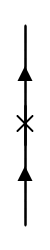
\includegraphics[height=3cm]{figures/diagramA.png}
		\caption{Diagram A}
	\end{subfigure}
	\begin{subfigure}{0.2\textwidth}
		\centering
		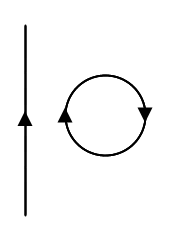
\includegraphics[height=3cm]{figures/diagramB.png}
		\caption{Diagram B}
	\end{subfigure}
	\begin{subfigure}{0.2\textwidth}
		\centering
		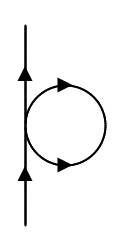
\includegraphics[height=3cm]{figures/diagramC.png}
		\caption{Diagram C}
	\end{subfigure}
	\begin{subfigure}{0.2\textwidth}
		\centering
		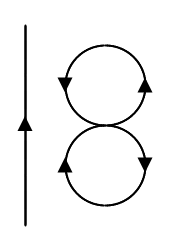
\includegraphics[height=3cm]{figures/diagramD.png}
		\caption{Diagram D}
	\end{subfigure}
\end{figure}

Additionally, we find that in the $w_{rs}$ case (A and B), there is always one incoming line and one outcoming line for each intermediate vertex, which is because of one creation operator and one annihilation operator in the expression $W=w_{rs} c_r^{\dagger} c_s$.
In the $V_{uvrs}$ case (C and D), there are always two incoming lines and two outcoming lines for rach intermediate vertex, which is because of two creation operators and two annihilation operators in the expression $V=\frac{1}{2}V_{uvrs} c_u^{\dagger} c_v^{\dagger} c_s c_r$.

Compared with the expressions, the diagrams are very simple, which is one of its advantages.
In fact, Feynman diagram can not only show the structure of expression, but can also restore all the algebraic details.
This means that, instead of doing any algebraic calculation, we can just draw all the possible diagrams and then use some rules to translate to algebraic results.
Then we will derive the rules:

For each vertex, we assign $w_{rs}$ or $V_{uv[rs]}$ depending on whether it's a $w$ vertex or a $V$ vertex:

\hspace{0.2\textwidth}
\begin{minipage}{0.08\textwidth}
	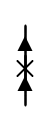
\includegraphics[height=3cm]{figures/vertexW.png}
\end{minipage}
\begin{minipage}{0.2\textwidth}
	$=w_{rs}$
\end{minipage}
\begin{minipage}{0.18\textwidth}
	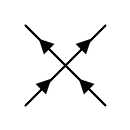
\includegraphics[height=3cm]{figures/vertexV.png}
\end{minipage}
\begin{minipage}{0.1\textwidth}
	$=V_{uv[rs]}$
\end{minipage}

It is easy to understand the result of $w$ vertex, since $W=w_{rs} c_r^{\dagger} c_s$.
For the $V$ case, $V=\frac{1}{2}V_{uvrs} c_u^{\dagger} c_v^{\dagger} c_s c_r$.
Wick's theorem states all possible of contraction should be included, thus any algebraic expression will have "partners" that the only difference is the exchange of index $u$ and $v$, or $s$ and $r$, or both.
Thus, instead of $\frac{1}{2}V_{uvrs}$, the proper magnitude should be $\frac{1}{2}V_{[uv][rs]}=V_{uv[rs]}$.

However, it is not always the case, since sometimes we will meet double counting.
For example in the double loop in Diagram D, which corresponds to algebraic expression
\begin{equation}
	\left\langle\Phi_{0}\left|
	\hat{\mathcal{T}}\left[
		c_{u}^{\dagger}\left(t_{1}\right) 
		c_{v}^{\dagger}\left(t_{1}\right)
		c_{s}\left(t_{1}\right) 
		c_{r}\left(t_{1}\right)
	\right]
	\right| \Phi_{0}\right\rangle
\end{equation}

Obviously, there is only two contraction schemes, i.e. $u$ with $s$, $v$ with $r$, or $u$ with $r$, $v$ with $s$. 
Thus, we meet double counting here.
Genrally, when two lines are equal, double counting happens.
Thus, the final result should be divided by two for each pair of equal lines.


Each line or curve is assigned by its corresponding Green function, which is also easy to understand.
In the case of higher orders, the expression is 
\begin{equation} \label{greenexp}
\begin{aligned}
	i \tilde{G}^n_{p q}\left(t, t^{\prime}\right)
	=& \frac{(-i)^{n}}{n !} 
	\int_{-\infty}^{\infty} \mathrm{d} t_{1} e^{-\epsilon\left|t_{1}\right|} \ldots \int_{-\infty}^{\infty} \mathrm{d} t_{n} e^{-\epsilon\left|t_{n}\right|}
	\\
	& \left\langle\Phi_{0}\left|
	\hat{\boldsymbol{T}}\left[\hat{H}_{I}\left(t_{1}\right) \ldots \hat{H}_{I}\left(t_{n}\right) c_{p}(t) c_{q}^{\dagger}\left(t^{\prime}\right)\right]\right|
	\Phi_{0}\right\rangle
\end{aligned}
\end{equation}
which has a factor of $\frac{(-i)^n}{n!}$.

However, $t_1 \dots t_n$ are treated on each footing and can also be exchanged when calculting the time-ordered product, thus it will contribute a factor $n!$.
Thus the overall factor is $(-i)^n$.

Last but not least, we need to determine the overall sign of the expression.
Unfortunately, it is impossible to determine the sign just from diagram, thus one must go back to any one of the algebraic expressions and then count how many times one need to commute creation and annihilation operator in the expression of time-ordered product.

Feynman diagram drawed by above rules is refered as Abrikosov diagram.

Then we go back to the calculation of first order Green function.
Let's first focus on expression B and D.
Both parts contain $G^0_{pq}(t,t^{\prime})$, which corresponds to a separate line in Diagram B and D.
Now we introduce the famous linked-cluster theorem, which states that all diagrams contain a separate $G^0_{pq}(t,t^{\prime}$ line will be canceled by the denominator of Eq \ref{greenexp}.
The proof is given in the reference \cite{main}.
Here we take first order Green function as an example.

Up to the first order, Green function can be written as
\begin{equation}
	\begin{aligned}
		i\tilde{G}_{pq}(t,t^{\prime})=&i \delta_{pq} G^0_{p}(t,t^{\prime})
		\\
		+&w_{pq} G^0_p(t,t_1) G^0_q(t_1,t^{\prime}) - w_{rr} G^0_r(t_1,t_1) \delta_{pq} G^0_{p}(t,t^{\prime})
		\\
		-&V_{pr[qr]} G^0_{p}(t,t_1) G^0_{r}(t_1,t_1) G^0_{q}(t_1,t^{\prime})
		- V_{rs[rs]} G^0_r(t_1,t_1) G^0_s(t_1,t_1) \delta_{pq} G^0_p(t,t^{\prime})
		\\
		+&O(2)
	\end{aligned}
\end{equation}
while the denominator is 
\begin{equation}
	\left\langle\Phi_{0}\left|\hat{U}_{\epsilon}(0,-\infty)\right| \Phi_{0}\right\rangle=1
		- w_{rr} G^0_r(t_1,t_1)
		- V_{rs[rs]} G^0_r(t_1,t_1) G^0_s(t_1,t_1)
		+ O(2)
\end{equation}

Thus up to the first order,  the overall Green function reads
\begin{equation}
	i G_{pq}(t,t^{\prime})=i \delta_{pq} G^0_{p}(t,t^{\prime})
	+w_{pq} G^0_p(t,t_1) G^0_q(t_1,t^{\prime})
	-V_{pr[qr]} G^0_{p}(t,t_1) G^0_{r}(t_1,t_1) G^0_{q}(t_1,t^{\prime}) +O(2)
\end{equation}
where all unlinked diagrams are canceled.

As we mentioned before, both the numerator and denominator contains divergent terms, which will be canceled after division.
In fact, the divergent parts are excatly the unlinked diagrams.
Thus, linked-cluster theorem decreases the number of diagrams we need to calculate, and also gurantees the result is finite and thus physical.

Then we analyze the rest terms of first order Green function:
\begin{equation}
	\begin{aligned}
		i G^1_{pq}(t,t^{\prime}) &= w_{pq} G^0_p(t,t_1) G^0_q(t_1,t^{\prime})
		-V_{pr[qr]} G^0_{p}(t,t_1) G^0_{r}(t_1,t_1) G^0_{q}(t_1,t^{\prime})
		\\
		&= G^0_p(t,t_1) G^0_q(t_1,t^{\prime}) (w_{pq}-V_{pr[qr]}G^0_r(t_1,t_1)
		\\
		&= G^0_p(t,t_1) G^0_q(t_1,t^{\prime}) (w_{pq}+V_{pr[qr]}n_r)
		\\
		&=0
	\end{aligned}
\end{equation}
where 
\begin{equation}
	\begin{aligned}
		G^0_r(t_1,t_1)&=G^0_r(t_1,t_1^{+})
		\\
		&=- \left\langle\Phi_{0}\left|
		c_r^{\dagger} c_r
		\right| \Phi_{0}\right\rangle
		\\
		&=-n_r
	\end{aligned}
\end{equation}
is used.

In fact, the diagrams that contain $w$ vertex will always cancel with the diagrams that cantain free Green function line starting and ending with the same $V$ vertex.
According to Eq \ref{greenexp}, $H_I$, which is $W$ and $V$ always appear together.
Thus, any diagram contain $V_{pr[qr]}n_r$ will automatically contain $r_{pq}$.
This result means that we can skip all diagrams with $W$ vertex and that cantain free Green function line starting and ending with the same $V$ vertex at the same time.
Thus, we will not consider $W$ vertex in the following.

Then we summarize the Feynman rules for Abrikosov diagram:
\begin{itemize}
	\item Draw all topologically distinct connected diagrams with $n$ interaction dots and $2n + 1$ directed (solid) free Green’s function starting at the outer vertex $(p, t)$ and ending at the outer vertex $(q, t^{\prime})$.
		At each interaction dot, two Green function start and two end; assign a time argument to each interaction dot.
	\item Attach one-particle indices and time arguments to the free Green function lines; the arrows define the order of the time arguments. Replace the graphical symbols (free Green function lines and interaction dots) by the respective analytical expressions.
	\item Sum over indices and integrate over time arguments of the inner vertices.
	\item The overall phase of an Abrikosov diagram can only be fixed by inspecting one of the Feynman diagrams comprised in the Abrikosov diagram.
		The phase is to be adapted in such a way that this Feynman diagram is reproduced correctly by the Abrikosov expression.
	\item Apply a factor of $\frac{1}{2}$ for each pair of (topologically) equivalent free Green function lines to compensate for double counting of Feynman diagrams. Double counting may arise for other reasons at fourth and higher order, and this possibility must be checked at the level of Feynman diagrams.
\end{itemize}

We calculate the second order Green function as the end of this section:
According to the Feynman diagram, we first draw all possible topologically inequvalent diagrams.
In the case of second order Green function, there is only one diagram:
\begin{figure}[h]
	\centering
	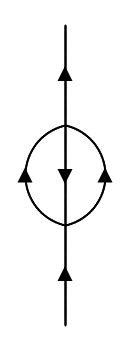
\includegraphics[height=4cm]{figures/order2.png}
	\caption{Diagram of second order Green function}
\end{figure}

Note that the two curves are identical ( start and end with the same vertexs).
Thus, according the Feynman rules, we can easily determine the second order Green function up to a overall sign:
\begin{equation} \label{order2}
	\begin{aligned} 
	G_{p q}^{(2)}\left(t, t^{\prime}\right)=\pm \frac{1}{2} \sum_{r, u, v_{-\infty}} & \int_{-\infty}^{\infty} \mathrm{d} t_{1} \int_{-\infty}^{\infty} \mathrm{d} t_{2} V_{p r[u v]} V_{u v[q r]} 
	\\ 
	& G_{p}^{0}\left(t, t_{1}\right) G_{u}^{0}\left(t_{1}, t_{2}\right) G_{v}^{0}\left(t_{1}, t_{2}\right) G_{r}^{0}\left(t_{2}, t_{1}\right) G_{q}^{0}\left(t_{2}, t^{\prime}\right) 
	\end{aligned}
\end{equation}

To determine the overall sign, we only need to consider the case
\begin{equation}
	\left\langle\Phi_{0}\left|
	\hat{\mathcal{T}}\left[
		\wick{\c4 c_{u}^{\dagger}\left(t_{1}\right) \c3 c_{v}^{\dagger}\left(t_{1}\right) \c2 c_{s}\left(t_{1}\right) \c1 c_{r}\left(t_{1}\right) \c1 c_{i}^{\dagger}\left(t_{2}\right) \c2 c_{j}^{\dagger}\left(t_{2}\right) \c3 c_{l}\left(t_{2}\right) \c1 c_{k}\left(t_{2}\right) \c4 c_{p}(t) \c1 c_{q}^{\dagger}\left(t^{\prime}\right)}
		\right]
		\right| \Phi_{0}\right\rangle
\end{equation}
which gives an overall sign of $-1$, which is canceled with the factor $(-i)^2$.

Thus the overall sign of expression Eq \ref{order2} should be positive.


\section{Algebraic Diagrammatic Construction}
With the basic knowledge of second quantization, perturbation theory and Green function, we can then start discussing ADC.
We know that we can calculate ionization potentials, electron affinities and ground state energy from Green function by \ref{spectralrepresentation} and \ref{greenenergy}.
We also know that we can use Wick's theorem and Feynman rules for Abrikosov diagram to calculate each order of Green function.
Thus, as least in principle, we can practically calculate some physical quantities.
However, a finite perturbation expansion, e.g., through third order, e.g.
\begin{equation}
\boldsymbol{G}(\omega)=\boldsymbol{G}^{0}(\omega)+\boldsymbol{G}^{(2)}(\omega)+\boldsymbol{G}^{(3)}(\omega)+O(4)
\end{equation}
does not result in a useful approximation scheme to determine the physical quantities of interest.
The reason is that the components $G_{pq}(ω)$ are analytical functions, and a finite perturbation expansion does not recover the proper analytical structure.
What is needed here is to sum the perturbation expansion, even if only partially, through infinite order.
We will introduce two ways, which are Dyson approach and Non-dyson approach to such infinite summation.

\subsection{Dyson Approach}
The Green function can be written as:

\begin{minipage}{0.08\textwidth}
	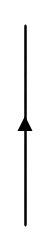
\includegraphics[height=3cm]{./figures/free.png}
\end{minipage}
\begin{minipage}{0.05\textwidth}
	+
\end{minipage}
\begin{minipage}{0.08\textwidth}
	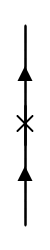
\includegraphics[height=3cm]{./figures/diagramA.png}
\end{minipage}
\begin{minipage}{0.05\textwidth}
	+
\end{minipage}
\begin{minipage}{0.12\textwidth}
	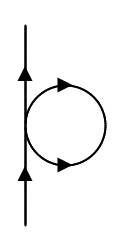
\includegraphics[height=3cm]{./figures/diagramC.png}
\end{minipage}
\begin{minipage}{0.05\textwidth}
	+
\end{minipage}
\begin{minipage}{0.1\textwidth}
	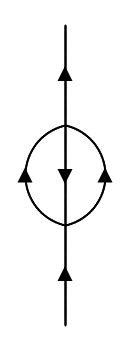
\includegraphics[height=3cm]{./figures/order2.png}
\end{minipage}
\begin{minipage}{0.2\textwidth}
	+ \qquad \dots
\end{minipage}

We can see that except the first one, all of the diagrams both start and end with a free Green function line.
Thus, we can define improper self-energy part $\widetilde{\Sigma}_{p q}\left(t_{1}, t_{1}^{\prime}\right)$ as the infinite summation of the parts between two free Green function lines in each diagram:

\hspace{0.4\textwidth}
\begin{minipage}{0.08\textwidth}
	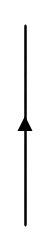
\includegraphics[height=3cm]{./figures/free.png}
\end{minipage}
\begin{minipage}{0.05\textwidth}
	+
\end{minipage}
\begin{minipage}{0.05\textwidth}
	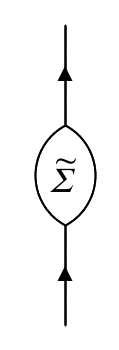
\includegraphics[height=3cm]{./figures/newdyson.png}
\end{minipage}

Algebraically, it reads:
\begin{equation}
	G_{p q}\left(t, t^{\prime}\right)=\delta_{p q} G_{p}^{0}\left(t, t^{\prime}\right)+\int \mathrm{d} t_{1} \int \mathrm{d} t_{1}^{\prime} G_{p}^{0}\left(t, t_{1}\right) \widetilde{\Sigma}_{p q}\left(t_{1}, t_{1}^{\prime}\right) G_{q}^{0}\left(t_{1}^{\prime}, t^{\prime}\right)
\end{equation}
or
\begin{equation}
	G_{p q}(\omega)=\delta_{p q} G_{p}^{0}(\omega)+G_{p}^{0}(\omega) \widetilde{\Sigma}_{p q}(\omega) G_{q}^{0}(\omega)
\end{equation}
in energy representation, or 
\begin{equation}
	\boldsymbol{G}(\omega)=\boldsymbol{G}^{0}(\omega)+\boldsymbol{G}^{0}(\omega) \widetilde{\boldsymbol{\Sigma}}(\omega) \boldsymbol{G}^{0}(\omega)
\end{equation}
in matrix representation.

To proceed to the definition of the less trivial proper self-energy part, let us consider the following fourth-order diagram.
\begin{figure}
	\centering
	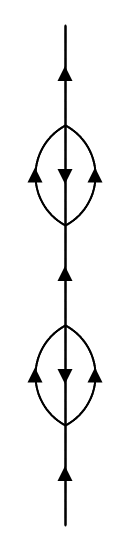
\includegraphics[height=6cm]{./figures/order4.png}
	\caption{one of fourth-order diagrams}
\end{figure}

It can be separated to two parts by a free Green function.
In a similar way, any diagram can be characterized as being either separable or non-separable with respect to cutting a single free fermion line. 
Thus, we can define the proper self-energy $\Sigma$ as summation over all non-separable diagrams.

Obviously, improper self-energy and proper self-energy are related by:

\begin{minipage}{0.12\textwidth}
	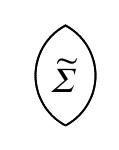
\includegraphics[height=2cm]{./figures/improper.png}
\end{minipage}
\begin{minipage}{0.02\textwidth}
	=
\end{minipage}
\begin{minipage}{0.12\textwidth}
	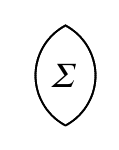
\includegraphics[height=2cm]{./figures/proper1.png}
\end{minipage}
\begin{minipage}{0.02\textwidth}
	+
\end{minipage}
\begin{minipage}{0.12\textwidth}
	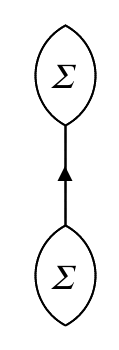
\includegraphics[height=4cm]{./figures/proper2.png}
\end{minipage}
\begin{minipage}{0.02\textwidth}
	+
\end{minipage}
\begin{minipage}{0.12\textwidth}
	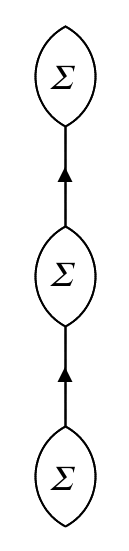
\includegraphics[height=6cm]{./figures/proper3.png}
\end{minipage}
\begin{minipage}{0.2\textwidth}
	+ \qquad \dots
\end{minipage}

or algebraically by
\begin{equation}
	\tilde{\boldsymbol{\Sigma}}(\omega)=\boldsymbol{\Sigma}(\omega)+\boldsymbol{\Sigma}(\omega) \boldsymbol{G}^0(\omega) \tilde{\boldsymbol{\Sigma}}(\omega)
\end{equation}

Thus we can obtain the Dyson equation:
\begin{equation}
	\boldsymbol{G}(\omega)=\boldsymbol{G}^{0}(\omega)+\boldsymbol{G}^{0}(\omega) \boldsymbol{\Sigma}(\omega) \boldsymbol{G}(\omega)
\end{equation}
and thus
\begin{equation}
	\boldsymbol{\Sigma}(\omega)=\boldsymbol{G}^{0}(\omega)^{-1}-\boldsymbol{G}(\omega)^{-1}
\end{equation}

Since both the improper and proper self-energy are defined by summation of diagrams, it is obvious that they can also be expanded just like Green functions.
For example, the second order of proper self-energy is
\begin{equation} \label{selforder2}
	\Sigma_{p q}^{(2)}(\omega)=\sum_{a, b, k} \frac{V_{p k[a b]} V_{a b[q k]}}{\omega+\epsilon_{k}-\epsilon_{a}-\epsilon_{b}+i \eta}+\sum_{a, k, l} \frac{V_{p a[k l]} V_{k l[q a]}}{\omega+\epsilon_{a}-\epsilon_{k}-\epsilon_{l}-i \eta}
\end{equation}

The self-energy can be written in a general form:
\begin{equation}
	\Sigma_{p q}(\omega)=\Sigma_{p q}(\infty)+M_{p q}(\omega)
\end{equation}
where $\Sigma_{p q}(\infty)$ and $M_{p q}(\omega)$ are refered to as dynamical part and static part, respectively.
It can be proved that $M_{pq}(\omega)$ can also be written in a spectral representation form:
\begin{equation}
	M_{p q}(\omega)=M_{p q}^{+}(\omega)+M_{p q}^{-}(\omega)=\sum_{\nu} \frac{m_{p}^{(\nu)} m_{q}^{(\nu) *}}{\omega-\omega_{\nu}+i \eta}+\sum_{\mu} \frac{m_{p}^{(\mu)} m_{q}^{(\mu) *}}{\omega-\omega_{\mu}-i \eta}
\end{equation}

The proof in given in reference \cite{Mpqproof1,Mpqproof2}.

If the infinite small $\eta$ is ignored, then 
\begin{equation}
	M_{p q}(\omega)=\sum_{\nu} \frac{m_{p}^{(\nu)} m_{q}^{(\nu) *}}{\omega-\omega_{\nu}}+\sum_{\mu} \frac{m_{p}^{(\mu)} m_{q}^{(\mu) *}}{\omega-\omega_{\mu}}
\end{equation}
and 
\begin{equation}
	G_{p q}(\omega)=\sum_{n} \frac{x_{p}^{n} x_{q}^{n *}}{\omega-e_{n}}
\end{equation}
where $n$ runs over both $N+1$ states and $N-1$ states.

Additionally,
\begin{equation}
	\begin{aligned}
		G_{p q}^{0}(\omega)&=\delta_{p q}\left(\frac{\overline{n}_{p}}{\omega-\varepsilon_{p}+i \eta}+\frac{n_{p}}{\omega-\varepsilon_{p}-i \eta}\right)
		\\
		&=\frac{\delta_{p q}}{\omega-\varepsilon_{p}}
	\end{aligned}
\end{equation}

In matrix representation,
\begin{equation}
	\boldsymbol{M}^{ \pm}(\omega)=\boldsymbol{m}^{ \pm \dagger}\left(\omega \mathbf{1}-\boldsymbol{\Omega}^{ \pm}\right)^{-1} \boldsymbol{m}^{ \pm}
\end{equation}
\begin{equation}
	\boldsymbol{G}(\omega)=\boldsymbol{x}(\omega \mathbf{1}-\boldsymbol{E})^{-1} \boldsymbol{x}^{\dagger}
\end{equation}
\begin{equation}
	\boldsymbol{G}^0(\omega)=(\omega \mathbf{1} - \boldsymbol{\epsilon})^{-1}
\end{equation}
and 
\begin{equation}
	\boldsymbol{x} \boldsymbol{x}^{\dagger}=1
\end{equation}

Since
\begin{equation}
	\begin{aligned} \boldsymbol{G}(\omega)^{-1} &=\omega\left[x\left(\mathbf{1}-\frac{\boldsymbol{E}}{\omega}\right)^{-1} \boldsymbol{x}^{\dagger}\right]^{-1} \\ &=\omega\left[\boldsymbol{x}\left(\mathbf{1}+\frac{\boldsymbol{E}}{\omega}+O\left(\omega^{-2}\right)\right) \boldsymbol{x}^{\dagger}\right]^{-1} \\ &=\omega\left[\mathbf{1}+\boldsymbol{x} \frac{\boldsymbol{E}}{\omega} \boldsymbol{x}^{\dagger}+O\left(\omega^{-2}\right)\right]^{-1}=\omega \mathbf{1}-x \boldsymbol{E} \boldsymbol{x}^{\dagger}+O\left(\frac{1}{\omega}\right) \end{aligned}
\end{equation}

We have 
\begin{equation}
	\begin{aligned}
		\boldsymbol{\Sigma}(\omega)&=\boldsymbol{G}^{0}(\omega)^{-1}-\boldsymbol{G}(\omega)^{-1}
		\\
		&=-\boldsymbol{\epsilon}+\boldsymbol{x} \boldsymbol{E} \boldsymbol{x}^{\dagger}+O\left(\frac{1}{\omega}\right)
	\end{aligned}
\end{equation}
and thus
\begin{equation}
	\boldsymbol{\Sigma}(\infty)=-\boldsymbol{\epsilon}+\boldsymbol{x} \boldsymbol{E} \boldsymbol{x}^{\dagger}
\end{equation}


As a result, the Dyson equation becomes:
\begin{equation}
	\boldsymbol{G}(\omega)=\left(\omega \mathbf{1}-\boldsymbol{\epsilon}-\boldsymbol{\Sigma}(\infty)-\boldsymbol{m}^{-\dagger}\left(\omega \mathbf{1}-\boldsymbol{\Omega}^{-}\right)^{-1} \boldsymbol{m}^{-}-\boldsymbol{m}^{+^{\dagger}}\left(\omega \mathbf{1}-\boldsymbol{\Omega}^{+}\right)^{-1} \boldsymbol{m}^{+}\right)^{-1}
\end{equation}

It can be proved that if we introduce Dyson secular matrix
\begin{equation} \label{matrixA}
	\boldsymbol{A}=\left( \begin{array}{ccc}{\boldsymbol{\epsilon}+\boldsymbol{\Sigma}(\infty)} & {\boldsymbol{m}^{-\dagger}} & {\boldsymbol{m}^{+\dagger}} \\ {\boldsymbol{m}^{-}} & {\boldsymbol{\Omega}^{-}} & {\mathbf{0}} \\ {\boldsymbol{m}^{+}} & {\mathbf{0}} & {\boldsymbol{\Omega}^{+}}\end{array}\right)
\end{equation}
then
\begin{equation}
	\boldsymbol{G}(\omega)=\left.(\omega \mathbf{1}-\boldsymbol{A})^{-1}\right|_{11}
\end{equation}
where the $11$ subscript means taking the upper left diagonal block.

Thus the energies interested, which are poles of $G$, are also poles of Dyson secular matrix $A$.
Then we can diagonalize the matrix A to determine the values of poles and thus the energies and eigenstates, which are transition amplitudes, i.e.
\begin{equation}
	\boldsymbol{A} \boldsymbol{X}=\boldsymbol{X} \boldsymbol{E}, \quad \boldsymbol{X}^{\dagger} \boldsymbol{X}=1
\end{equation}

from Eq \ref{selforder2}, we can also determine the leading terms of $m$ and $\Omega$.
Since 
\begin{equation}
	\begin{aligned} 
	M_{p q}^{(2)+}(\omega) &=\sum_{a<b, k} \frac{V_{p k[a b]} V_{a b[q k]}}{\omega+\epsilon_{k}-\epsilon_{a}-\epsilon_{b}+i \eta}
	\\ 
	M_{p q}^{(2)-}(\omega) &=\sum_{a, k<l} \frac{V_{p a[k l]} V_{k l[q a]}}{\omega+\epsilon_{a}-\epsilon_{k}-\epsilon_{l}-\epsilon_{l}-i \eta}
	\end{aligned}
\end{equation}
we have
\begin{equation}
	\begin{aligned} 
	\Omega_{a k l, a k l}^{-} &=-\epsilon_{a}+\epsilon_{k}+\epsilon_{l}
	\\ 
	\Omega_{a b k, a b k}^{+} &=-\epsilon_{k}+\epsilon_{a}+\epsilon_{b} 
	\end{aligned}
\end{equation}
and
\begin{equation} 
	m_{a k l, q}^{-} =V_{q a[k l]}, \quad m_{a b k, q}^{+}=V_{a b[q k]}
\end{equation}

They are leading terms since the leading order of $M$ is second order.
This is because
\begin{equation}
	\begin{aligned}
		\boldsymbol{\Sigma}(\omega)&=\boldsymbol{G}^{0}(\omega)^{-1}-\boldsymbol{G}(\omega)^{-1}
		\\
		&=\boldsymbol{G}^{0}(\omega)^{-1}-(\boldsymbol{G}^0(\omega)+O(2))^{-1}
		\\
		&=O(2)
	\end{aligned}
\end{equation}

As is mentioned previously, a finite perturbation expansion of the electron propagator does not reproduce its correct analytical form.
However, we are still using finite perturbation expansion, i.e. determine each order of $m$, $\Omega$ and then calculate the eigenvalues of Dyson secular matrix in Eq \ref{matrixA}.

We will then begin introducing ADC to sum partially to infinity.
We will consider $M^{+}$ in the following since it is analogous for $M^{-}$.

In ADC, equation 
\begin{equation}
	M_{p q}(\omega)=\boldsymbol{m}_{p}^{\dagger}(\omega \mathbf{1}-\boldsymbol{\Omega})^{-1} \boldsymbol{m}_{q}
\end{equation}
is replaced by ADC form:
\begin{equation}
	M_{p q}(\omega)=\boldsymbol{U}_{p}^{\dagger}(\omega \mathbf{1}-\boldsymbol{K}-\boldsymbol{C})^{-1} \boldsymbol{U}_{q}
\end{equation}
where
$\boldsymbol{K}+\boldsymbol{C}$ is refered to as ADC secular matrix.

Although $\boldsymbol{K}$, $\boldsymbol{C}$, and $\boldsymbol{U}$ are not specified yet,
we may suppose that the following perturbation expansions apply:
\begin{equation} \label{cuexpansion}
	\begin{aligned} 
		\boldsymbol{C} &=\boldsymbol{C}^{(1)}+\boldsymbol{C}^{(2)}+\cdots 
		\\ 
		\boldsymbol{U_{p}} &=\boldsymbol{U_{p}}^{(1)}+\boldsymbol{U_{p}}^{(2)}+\cdots
	\end{aligned}
\end{equation}

Here $\boldsymbol{K}$ is actually the zeroth order of $\boldsymbol{C}$.
Thus
\begin{equation}
	\begin{array}{l}{K_{j a b, j a b}=-\epsilon_{j}+\epsilon_{a}+\epsilon_{b}} \\ {K_{i j a b c, i j a b c}=-\epsilon_{i}-\epsilon_{j}+\epsilon_{a}+\epsilon_{b}+\epsilon_{c}} \\ {\qquad \vdots}\end{array}
\end{equation}
where $i, j, k \dots$ label occupied orbitals while $a, b, c \dots$ label virtual orbitals.

Although we still expand $\boldsymbol{K}$ and $\boldsymbol{C}$ to finite order, the expansion of $M$ is already partially to infinite orders:
\begin{equation} \label{adcexpansion}
	\begin{aligned} M_{p q}(\omega) &=\boldsymbol{U}_{p}^{\dagger}(\omega \mathbf{1}-\boldsymbol{K}-\boldsymbol{C})^{-1} \boldsymbol{U}_{q} \\ &=\boldsymbol{U}_{p}^{\dagger}(\omega \mathbf{1}-\boldsymbol{K})^{-1} \sum_{n=0}^{\infty}\left\{\boldsymbol{C}(\omega \mathbf{1}-\boldsymbol{K})^{-1}\right\}^{n} \boldsymbol{U}_{q} \end{aligned}
\end{equation}

Now, we can formulate the ADC procedure as follows:

Compare the formal perturbation expansion of the ADC form Eq \ref{adcexpansion} to the original diagrammatic perturbation expansion for the self-energy part $M^{+}_{pq}(\omega)$ through a given order $n$ of perturbation theory.
Beginning at second order and proceeding to higher order, this comparison allows one to determine successively the terms in the expansions Eq \ref{cuexpansion} of $\boldsymbol{C}$ and $\boldsymbol{U}_p$ , respectively.

Through second order of $M$, we can determine $\boldsymbol{C}$ and $\boldsymbol{U}_p$ as
\begin{equation}
	U_{j a b, q}^{(1)}=V_{a b[q j]}
\end{equation}
\begin{equation}
	C_{j a b, j^{\prime} a^{\prime} b^{\prime}}=0
\end{equation}

Through third order of $M$, we can determine $\boldsymbol{C}$ and $\boldsymbol{U}_p$ as
\begin{equation}
	\begin{aligned} 
		U_{j a b, q}^{(2)}&= \frac{1}{2} \sum_{k l} \frac{V_{a b[k l]} V_{k l[q j]}}{\epsilon_{k}+\epsilon_{l}-\epsilon_{a}-\epsilon_{b}} +\left(\sum_{c k} \frac{V_{a c[k j]} V_{k b[q c]}}{\epsilon_{a}+\epsilon_{c}-\epsilon_{j}-\epsilon_{k}}\right)-(a \leftrightarrow b)
		\\
		C_{j a b, j^{\prime} a^{\prime} b^{\prime}}^{(1)}&=\delta_{j j^{\prime}} V_{a b\left[a^{\prime} b^{\prime}\right]}-\left(\delta_{a a^{\prime}} V_{j^{\prime} b\left[j b^{\prime}\right]}+\delta_{b b^{\prime}} V_{j^{\prime} a\left[j a^{\prime}\right]}\right)+(a^{\prime} \leftrightarrow b^{\prime})
	 \end{aligned}
\end{equation}

Instead of Dyson secular matrix, we have a new Dyson-ADC secular matrix:
\begin{equation}
	\boldsymbol{B}=\left( \begin{array}{ccc}{\epsilon+\mathbf{\Sigma}(\infty)} & {\boldsymbol{U}^{-\dagger}} & {\boldsymbol{U}^{+\dagger}} \\ {\boldsymbol{U}^{-}} & {\boldsymbol{K}^{-}+\boldsymbol{C}^{-}} & {\mathbf{0}} \\ {\boldsymbol{U}^{+}} & {\boldsymbol{0}} & {\boldsymbol{K}^{+}+\boldsymbol{C}^{+}}\end{array}\right)
\end{equation}
and
\begin{equation}
	\boldsymbol{G}(\omega)=\left.(\omega \mathbf{1}-\boldsymbol{B})^{-1}\right|_{11}
\end{equation}
and thus diagonalization as
\begin{equation}
	\boldsymbol{B} \boldsymbol{X}=\boldsymbol{X} \boldsymbol{E}, \quad \boldsymbol{X}^{\dagger} \boldsymbol{X}=1
\end{equation}

The structure of Dyson-ADC(3) matrix is:
\begin{table}
	\centering
	\caption{Structure of Dyson-ADC(3)}
\begin{tabular}{cccc}
                           & 1h/1p                                                                    & 2h-1p                                    & 2p-1h                                      \\ \cline{2-4} 
\multicolumn{1}{c|}{1h/1p} & \multicolumn{1}{c|}{$\boldsymbol{\epsilon}+\boldsymbol{\Sigma}(\infty)$} & \multicolumn{1}{c|}{$U^{-(1,2)\dagger}$} & \multicolumn{1}{c|}{$ U^{+(1,2)\dagger} $} \\ \cline{2-4} 
\multicolumn{1}{c|}{2h-1p} & \multicolumn{1}{c|}{$U^{-(1,2)}$}                                        & \multicolumn{1}{c|}{$K^{-}+C^{-(1)}$}    & \multicolumn{1}{c|}{0}                     \\ \cline{2-4} 
\multicolumn{1}{c|}{2p-1h} & \multicolumn{1}{c|}{$U^{+(1,2)}$}                                        & \multicolumn{1}{c|}{0}                   & \multicolumn{1}{c|}{$K^{+}+C^{+(1)}$}      \\ \cline{2-4} 
\end{tabular}
\end{table}

The summation to infinity ensures that Dyson-ADC is a size consistent method, which is an important advantage over CI.
Another advantage is that configuration space of Dyson-ADC is smaller than CI.
For example, The consistent treatment of 1h main states through second (and third order) requires the CI expansions to extend through the 3h-2p configurations.
By contrast, the ADC(2) (and ADC(3)) configuration spaces are restricted to the 2h-1p configurations of $N−1$ particles, but also comprise the 2h-1p configurations of $N+1$ particles.

\subsection{Non-dyson Approach}
The advantage of Dyson approach is the decrease the number of Feynman diagrams one need to calculate by property of Dyson equation.
However, the problem is that $N+1$ part and $N-1$ part are coupled, thus one has to diagonalize the full B matrix.
Moreover, people usually care about the first few ionized or anionized states, which lie in the middle of the energy spectrum.
Algorithmically, it is difficult to determine eigenvalues in the middle part of an energy spectrum.
Thus, we introduce Non-dyson approach, which solve this problem and make sure that all states interested are in the edge of energy spectrum
Since Non-dyson ADC treat $N+1$ part and $N-1$ part separately, we will focus on $N-1$ part, and $N+1$ part is analogous.

Related to $N-1$ part, Green function $G^{-}$ can be written as
\begin{equation}
	\boldsymbol{G}^{-}(\omega)=\boldsymbol{x}(\omega \mathbf{1}-\boldsymbol{\Omega})^{-1} \boldsymbol{x}^{\dagger}
\end{equation}
where $\Omega$ are negative ionization energies that we do care about.

By transposing, we obtain
\begin{equation}
	\tilde{\boldsymbol{G}}(\omega)=\boldsymbol{G}^{-}(\omega)^{t}=\tilde{\boldsymbol{x}}^{\dagger}(\omega \mathbf{1}-\boldsymbol{\Omega})^{-1} \tilde{\boldsymbol{x}}
\end{equation}

Then we introduce ADC representation just like Dyson approach:
\begin{equation}
	\tilde{\boldsymbol{G}}(\omega)=\boldsymbol{f}^{\dagger}(\omega-\boldsymbol{K}-\boldsymbol{C})^{-1} \boldsymbol{f}
\end{equation}
and diagonalization as
\begin{equation} \label{KCeigen}
	(\boldsymbol{K}+\boldsymbol{C}) \boldsymbol{X}=\boldsymbol{X} \boldsymbol{E}, \quad \boldsymbol{X}^{\dagger} \boldsymbol{X}=1
\end{equation}

Just like Dyson approach, we still expand $\boldsymbol{C}$ and $\boldsymbol{g}$ to series:
\begin{equation}
	\begin{aligned} \boldsymbol{K}+\boldsymbol{C} &=\boldsymbol{K}+\boldsymbol{C}^{(1)}+\boldsymbol{C}^{(2)}+\boldsymbol{C}^{(3)}+\ldots \\ \boldsymbol{f} &=\boldsymbol{f}^{(0)}+\boldsymbol{f}^{(1)}+\boldsymbol{f}^{(2)}+\ldots \end{aligned}
\end{equation}
where the expression for $\boldsymbol{K}$ is:
\begin{equation}
	\begin{aligned} K_{k k} &=\epsilon_{k} \\ K_{a k l, a k l} &=\epsilon_{k}+\epsilon_{l}-\epsilon_{a} \\ & \vdots \end{aligned}
\end{equation}

Just like Dyson approach, we can also see that the expansion of $M$ is partially to infinite orders:
\begin{equation}
	\tilde{\boldsymbol{G}}(\omega)=\boldsymbol{f}^{\dagger}(\omega-\boldsymbol{K}-\boldsymbol{C})^{-1} \boldsymbol{f}=\boldsymbol{f}^{\dagger}(\omega-\boldsymbol{K})^{-1} \sum_{\nu=0}^{\infty}\left(\frac{\boldsymbol{C}}{\omega-\boldsymbol{K}}\right)^{\nu} \boldsymbol{f}
\end{equation}

The procedure of Non-dyson ADC is the same with Dyson-ADC.
By this procedure, we obtain the first few orders of $\boldsymbol{C}$ and $\boldsymbol{f}$ for Non-dyson ADC(2):

\begin{equation}
	\begin{aligned}
		f_{p q}^{(0)}&=\delta_{p q} n_{p}
		\\
		f_{\mu}^{(0)}&=0, \text { for } \mu>1
		\\
		f_{1}^{(1)}&=0 \text { for } \mu>2
		\\
		f_{a k l, q}^{(1)}&=\frac{V_{q a[k] ]}}{\epsilon_{q}+\epsilon_{a}-\epsilon_{k}-\epsilon_{l}} \overline{n}_{q}
		\\
		f_{p q}^{(2)}&=\frac{1}{4} \sum_{a, b, j} v_{a b p j} v_{q j a b} n_{q}
		\\
		C_{11}^{(1)}&=0
		\\
		C_{1 \mu}^{(1)}&=0 \text { for } \mu>2
		\\
		C_{p, a k l}^{(1)}&=-V_{k l[p a]} n_{p}
		\\
		C_{p q}^{(2)}&=\frac{1}{2} \sum_{a, b, j} v_{a b p j} v_{q j a b}\left(\epsilon_{a}+\epsilon_{b}-\epsilon_{j}-\frac{1}{2} \epsilon_{p}-\frac{1}{2} \epsilon_{q}\right), n_{p}=n_{q}=1
	\end{aligned}
\end{equation}

The structure of Non-dyson ADC(2) matrix is:
\begin{table}
	\centering
	\caption{Structure of Non-dyson ADC(2)}
	\label{ADC2}
	\begin{tabular}{ccc}
						       &             1p                      &             1h-2p               \\ \cline{2-3} 
	\multicolumn{1}{l|}{1p   } & \multicolumn{1}{l|}{$K_1+C^2_{11}$} & \multicolumn{1}{l|}{$C^1_{12}$} \\ \cline{2-3} 
	\multicolumn{1}{l|}{1h-2p} & \multicolumn{1}{l|}{$C^1_{21}$}     & \multicolumn{1}{l|}{$K_2$}      \\ \cline{2-3} 
	\end{tabular}
\end{table}

The structure of Non-dyson ADC(3) matrix is:
\begin{table}
	\centering
	\caption{Structure of Non-dyson ADC(3)}
	\label{ADC3}
	\begin{tabular}{ccc}
						           &                     1p                       &                     1h-2p                \\ \cline{2-3} 
		\multicolumn{1}{l|}{1p   } & \multicolumn{1}{l|}{$K_1+C^2_{11}+C^3_{11}$} & \multicolumn{1}{l|}{$C^1_{12}+C^2_{12}$} \\ \cline{2-3} 
		\multicolumn{1}{l|}{1h-2p} & \multicolumn{1}{l|}{$C^1_{21}+C^2_{12}$}     & \multicolumn{1}{l|}{$K_2+C^1_{22}$}      \\ \cline{2-3} 
	\end{tabular}
\end{table}

We can also use \ref{greenenergy} to calculate ground state energy by Non-dyson ADC.
\begin{equation}
	\begin{aligned}
		\boldsymbol{\rho}&=\frac{1}{2 \pi i} \oint \boldsymbol{G}^{-}(\omega) \mathrm{d} \omega
		\\
		&=\frac{1}{2 \pi i} \oint \boldsymbol{f}^{\dagger}(\omega-\boldsymbol{K}-\boldsymbol{C})^{-1} \boldsymbol{f} \mathrm{d} \omega=\boldsymbol{f}^{\dagger} \boldsymbol{f}
	\end{aligned}
\end{equation}

Thus
\begin{equation}
	E_{0}=\frac{1}{2} \operatorname{Tr}\left(\boldsymbol{f}^{\dagger}(\boldsymbol{K}+\boldsymbol{C}) \boldsymbol{f}+\boldsymbol{T}^{t} \boldsymbol{f}^{\dagger} \boldsymbol{f}\right)
\end{equation}

The complexity of Non-dyson ADC(2) is $m^4$ while ADC(3) is $m^5$, where $m$ is the number of one particle basis.

It can be proved that Non-dyson ADC is also size consistent.
The reason is that the direct ADC secular matrix can be identified as the representation of the (subtracted) Hamiltonian with respect to a specific set of intermediate states, which will be presented in the next section.


\section{Intermediate State Representation}

In Non-dyson ADC method, the eigenvalues of ADC secular matrix $\boldsymbol{K}+\boldsymbol{C}$ are exactly the ionization potentials, which behaves similar to Hamiltonian.
This feature suggests that $\boldsymbol{K}+\boldsymbol{C}$ is essentially a representation of Hamiltonian in some particular basis.
The surprising answer is that ADC secular equations can be deduced by a wavefunction approach, and the basis are refered to intermediate-state representation (ISR).
In addition, ISR approach allows us to analyze the origin of the compactness and size consistency of ADC.

We start from the so-called correlated excited (CE) states, which is defined by
\begin{equation}
	| \Psi_{J}^{0} \rangle=\hat{C}_{J} | \Psi_{0} \rangle
\end{equation}
where
\begin{equation}
	\left\{\hat{C}_{J}\right\}=\left\{c_{k} ; c_{a}^{\dagger} c_{k} c_{l}, k<l ; c_{a}^{\dagger} c_{b}^{\dagger} c_{j} c_{l} c_{l}, a<b, j<k<l ; \ldots\right\}
\end{equation}

Obviously, CE states are not orthogonal:
\begin{equation}
	S_{I J}=\langle\Psi_{I}^{0} | \Psi_{J}^{0}\rangle=\langle\Psi_{0}|\hat{C}_{I}^{\dagger} \hat{C}_{J}| \Psi_{0}\rangle \neq \delta_{I, J}
\end{equation}

Instead of the most obvious symmetric orthonormalization choice, which is 
\begin{equation}
	| \overline{\Psi}_{J} \rangle=\sum_{I} | \Psi_{I}^{0} \rangle\left(S^{-1 / 2}\right)_{I J}
\end{equation}
, we orthogonalize them by excitation class orthogonalization (ECO) procedure which states as follows:

\begin{itemize}
	\item First we construct intermediate states $\ket{\Psi^{\#}_K}$ by class. For states in class 1, we leave them unchanged, i.e.
		\begin{equation}
			\ket{\Psi^{\#}_i}=\ket{\Psi^0_i}
		\end{equation}
		Assuming intermediate states of classes 1, ..., $\nu-1$ have been constructed, then we orthogonalize $\ket{\tilde{\Psi}_J}$ in class $\nu$ by
		\begin{equation}
			| \Psi_{J}^{\#} \rangle=| \Psi_{J}^{0} \rangle-\sum_{[K]<\nu} | \Psi^{\#}_{K} \rangle\langle\Psi^{\#}_{K} | \Psi_{J}^{0}\rangle
		\end{equation}
	\item Orthogonalize states in each class by symmetric orthogonalization:
		\begin{equation}
			| \tilde{\Psi}_{J} \rangle=\sum_{[I]=\nu} | \Psi_{I}^{\#} \rangle\left(S_{\nu}^{-1 / 2}\right)_{I J}
		\end{equation}
\end{itemize}
where intermediate normalization is chosen.
\begin{equation}
	\langle\Psi_{0} | \Phi_{0}\rangle= 1
\end{equation}

Define ISR secular matrix $M$ by
\begin{equation}
	M_{I J}=\langle\tilde{\Psi}_{I}|\hat{H}-E_{0}| \tilde{\Psi}_{J}\rangle
\end{equation}
and 
\begin{equation}
	| \Psi_{n}^{N-1} \rangle=\sum_{I} X_{I n} | \tilde{\Psi}_{I} \rangle
\end{equation}

In matrix notation, the ISR secular equations take on the form
\begin{equation}
	\boldsymbol{M X}=\boldsymbol{X} \boldsymbol{\Omega}, \boldsymbol{X}^{\dagger} \boldsymbol{X}=\mathbf{1}
\end{equation}

Define ISR transition amplitudes as
\begin{equation}
	\tilde{f}_{I p}=\langle\tilde{\Psi}_{I}|c_{p}| \Psi_{0}\rangle
\end{equation}
with its relation to spectroscopic factor as
\begin{equation}
	x_{p}^{(n)}=\sum_{I} X_{I n}^{*} \tilde{f}_{I p}
\end{equation}

It can be proved that the ADC and ECO-ISR secular matrices are to be identified according to
\begin{equation}
	\begin{aligned} \boldsymbol{K}+\boldsymbol{C} & \equiv-\boldsymbol{M} \\ \boldsymbol{f} & \equiv \tilde{\boldsymbol{f}} \end{aligned}
\end{equation}

Although it is difficult to prove, one can check the second order of $M$ to verify it.
The verification is done in \cite{main}.

The equivalence of Non-dyson ADC and ISR approach results in two important features of ADC.
One is the compactness of matrix structure, which is the consequence of the so-called canonical perturbation theory order structure.
Compactness reduces the complexity of algorithm by reducing the size of total configuration space
The other is self consistency, which is guaranteed by the separability of ISR.
As is previously mentioned, self consistency ensures results of many important chemical processes calculation much more reliable.

Through out the calculation of $C$ and $f$ in each order, we find that they do not always begin from the zeroth order.
In fact, the leading order is dependent on the distance of the classes of two  indexes.
This rule states as follows:
\begin{equation}
	M_{I J} \sim O( | [I]-[J] | )
\end{equation}
which is also refered to as canonical order relations (COR).

For example, in CI matrix, the matrix element of class 1 and class 3 is in the first order, which breaks COR:
\begin{equation}
	H_{i, a b j k l}=\langle\Phi_{i}|\hat{H}_{I}| \Phi_{a b j k l}\rangle=-\delta_{i j} V_{k l[a b]}+\delta_{i k} V_{j I l[a b]}-\delta_{i l} V_{j k[a b]}
\end{equation}
while in the case of ISR,
\begin{equation}
	\begin{aligned} M_{i, a b j k l}^{(1)} &=\langle\tilde{\Psi}_{i}|\hat{H}-E_{0}| \tilde{\Psi}_{a b j k l}\rangle^{(1)} \\ &=H_{i, a b j k l}+\langle\tilde{\Psi}_{i}^{(1)}|\hat{H}_{0}-E_{0}^{(0)}| \Phi_{a b j k l}\rangle+\langle\Phi_{i}|\hat{H}_{0}-E_{0}^{(0)}| \tilde{\Psi}_{a b j k l}^{(1)}\rangle \end{aligned}
\end{equation}

According to ECO procedure,
\begin{equation}
	| \tilde{\Psi}_{i}^{(1)} \rangle=c_{i} | \Psi_{0}^{(1)} \rangle
\end{equation}
and
\begin{equation}
	\begin{aligned} | \tilde{\Psi}_{a b j k l}^{(1)} \rangle &=c_{a}^{\dagger} c_{b}^{\dagger} c_{j} c_{k} c_{l} | \Psi_{0}^{(1)} \rangle-| \Phi_{j} \rangle\langle\tilde{\Psi}_{j}^{(1)} | \Phi_{a b j k l}\rangle-| \Phi_{k} \rangle\langle\tilde{\Psi}_{k}^{(1)} | \Phi_{a b j k l}\rangle-| \Phi_{l} \rangle\langle\tilde{\Psi}_{l}^{(1)} | \Phi_{a b j k l}\rangle \\ &= c_{a}^{\dagger} c_{b}^{\dagger} c_{j} c_{k} c_{l} | \Psi_{0}^{(1)} \rangle-| \Phi_{j} \rangle v_{a b k l}^{*}+| \Phi_{k} \rangle_{a b j l}^{*}-| \Phi_{l} \rangle v_{a b j k}^{*} \end{aligned}
\end{equation}
where there are no first-order contributions from the orthogonalization with
respect to 2h-1p states.

Thus
\begin{equation}
	\langle\Phi_{i}|\hat{H}_{0}-E_{0}^{(0)}| \tilde{\Psi}_{a b j k l}^{(1)}\rangle=-\epsilon_{i}\langle\Phi_{i} | \tilde{\Psi}_{a b j k l}^{(1)}\rangle=\epsilon_{i}\left(\delta_{i j} v_{a b k l}^{*}-\delta_{i k} v_{a b j l}^{*}+\delta_{i l} v_{a b j k}^{*}\right)
\end{equation}
and
\begin{equation}
	\langle\tilde{\Psi}_{i}^{(1)}|\hat{H}_{0}-E_{0}^{(0)}| \Phi_{a b j k l}\rangle=\left(\delta_{i j} v_{a b k l}^{*}-\delta_{i k} v_{a b j l}^{*}+\delta_{i l} v_{a b j k}^{*}\right)\left(\epsilon_{a}+\epsilon_{b}-\epsilon_{j}-\epsilon_{k}-\epsilon_{l}\right)
\end{equation}

Adding these three up gives:
\begin{equation}
	M_{i, a b j k l}^{(1)}=0
\end{equation}

The general proof of COR for ADC is given in refernce \cite{main}.

Thus, if configuration space from class 1 to class $\mu$ is fully included, the truncation error order (TEO) of energies in 1h class is
\begin{equation}
	O_{T E}^{[n]}(\mu)=2\mu
\end{equation}
where TEO means the leading order of error.

A generalized form of this relation is TEO for in $n$th class is
\begin{equation} \label{generalTEO}
	O_{T E}^{[n]}(\mu)=2(\mu-n)
\end{equation}

While the CI case, 
\begin{equation}
H_{IJ}=\left\{ 
\begin{array}{ll}
	O(0), & \text{ } I=J
	\\
	O(1), & \text{ } |I-J|=1 \text{ or } 2
	\\
	0,    & \text{ } |I-J|>2
\end{array}
\right.
\end{equation}
which gives the TEO as
\begin{equation}
	O_{T E}(\mu)=\left\{\begin{array}{ll}{\mu,} & {\mu \text { even }} \\ {\mu+1,} & {\mu \text { odd }}\end{array}\right.
\end{equation}
which is a much larger error than ADC case.

Then we will discuss the size consistency of Non-dyson ADC.
Size consistency of Non-dyson ADC replies on two facts.

The first is factorization theorem, which states that intermediate state of system A+B is the direct product of that of A and B, i.e.
\begin{equation}
	| \tilde{\Psi}_{J_{A B}} \rangle=| \tilde{\Psi}_{J_{A}}^{A} \rangle | \tilde{\Psi}_{J_{B}}^{B} \rangle
\end{equation}
where $| \tilde{\Psi}_{J_{A B}} \rangle$ comes from
\begin{equation}
	| \Psi_{J_{A B}}^{0} \rangle=\hat{C}_{J_{A B}} | \Psi_{0} \rangle=\hat{C}_{J_{A}} | \Psi_{0}^{A} \rangle \hat{C}_{J_{B}} | \Psi_{0}^{B} \rangle
\end{equation}
and the same for $| \tilde{\Psi}_{J_{A}}^{0} \rangle$ and $| \tilde{\Psi}_{J_{B}}^{0} \rangle$.

The second is the separability of ADC secular matrix, which means excitation of only A, excitation of only B and excitation of both A and B are three independent diagonal blocks in ADC secular matrix, i.e. the following structure.
\begin{equation}
	\begin{array}{|c|c|c|}
		\hline
		M_{AA} & 0 & 0
		\\
		\hline
		0 & M_{BB} & 0
		\\
		\hline
		0 & 0 & M_{AB,AB}
		\\
		\hline
	\end{array}
\end{equation}

We will then prove each of them and also illustrate how do they relate to size consistency of ADC.

The full proof of factorization is in reference \cite{sizeproof}.
Then we take an example of 1h of A and 1h1p of B to see how does it work.
The corresponding CE state reads:
\begin{equation}
	| \Psi_{a^{\prime} j^{\prime} k}^{0} \rangle=c_{k} | \Psi_{0}^{A} \rangle c_{a^{\prime}}^{\dagger} c_{j^{\prime}} | \Psi_{0}^{B} \rangle
\end{equation}

The first step of ECO gives
\begin{equation}
	| \Psi_{a^{\prime} j^{\prime} k}^{\#} \rangle=| \Psi_{a^{\prime} j^{\prime} k}^{0} \rangle-\sum_{l} | \tilde{\Psi}_{l} \rangle\langle\tilde{\Psi}_{l} | \Psi_{a^{\prime} j^{\prime} k}^{0}\rangle
\end{equation}
where
\begin{equation}
	| \tilde{\Psi}_{l} \rangle=| \tilde{\Psi}_{l}^{A} \rangle | \Psi_{0}^{B} \rangle
\end{equation}

Thus
\begin{equation}
	\begin{aligned} 
		| \Psi_{a^{\prime} j^{\prime} k}^{\#} \rangle 
		&=c_{k} | \Psi_{0}^{A} \rangle c_{a^{\prime}}^{\dagger} c_{j^{\prime}} | \Psi_{0}^{B} \rangle-\sum_{l} | \tilde{\Psi}_{l}^{A} \rangle\langle\tilde{\Psi}_{l}^{A}|c_{k}| \Psi_{0}^{A}\rangle | \Psi_{0}^{B} \rangle\langle\Psi_{0}^{B}|c_{a^{\prime}}^{\dagger} c_{j^{\prime}}| \Psi_{0}^{B}\rangle 
		\\ 
		&= c_{k} | \Psi_{0}^{A} \rangle\left(c_{a^{\prime}}^{\dagger} c_{j^{\prime}} | \Psi_{0}^{B}\rangle-| \Psi_{0}^{B} \rangle\langle\Psi_{0}^{B}|c_{a^{\prime}}^{\dagger}| \Psi_{0}^{B}\rangle \right)
		\\
		&=| \Psi_{k}^{A \#} \rangle | \Psi_{a^{\prime} j^{\prime}}^{B \#} \rangle
	\end{aligned}
\end{equation}

Thus, after symmetric orthogonalization, the intermediate states of A+B will still be the direct product of that of A and B.
\begin{equation}
	| \tilde{\Psi}_{a^{\prime} j^{\prime} k} \rangle=| \tilde{\Psi}_{k}^{A} \rangle | \tilde{\Psi}_{a^{\prime} j^{\prime}}^{B} \rangle
\end{equation}

To prove the separability, we need to prove that $M_{I_A J_B}=0$, $M_{I_A, J_{AB}}=0$ and $M_{I_B J_{AB}}=0$.
Since A and B are treated on equal footing, we only need to prove the first two.
\begin{equation}
	M_{I_{A}, J_{B}}=\langle\tilde{\Psi}_{I_{A}}|\hat{H}| \tilde{\Psi}_{J_{B}}\rangle=\langle\tilde{\Psi}_{I_{A}}^{A}|\langle\Psi_{0}^{B}|\left(\hat{H}_{A}+\hat{H}_{B}\right)| \tilde{\Psi}_{J_{B}}^{B}\rangle| \Psi_{0}^{A}\rangle= 0
\end{equation}
\begin{equation}
	\begin{aligned}
		M_{I_{A}, J_{A B}} &=\langle\tilde{\Psi}_{I_{A}}|\hat{H}| \tilde{\Psi}_{J_{A B}}\rangle 
		\\
		&=\langle\tilde{\Psi}_{I_{A}}^{A}|\langle\Psi_{0}^{B}|\left(\hat{H}_{A}+\hat{H}_{B}\right)| \tilde{\Psi}_{J_{A}}^{A}\rangle| \tilde{\Psi}_{J_{B}}^{B}\rangle 
		\\
		&=\langle\tilde{\Psi}_{I_{S}}^{A} | \hat{H}_A | \tilde{\Psi}_{J_{A}}^{A}\rangle \langle\Psi_{0}^{B} | \tilde{\Psi}_{J_{B}}^{B}\rangle
		+\langle\tilde{\Psi}_{I_{A}}^{A} | \tilde{\Psi}_{J_{A}}^{A}\rangle \langle\Psi_{0}^{B}|\hat{H}_{B}| \tilde{\Psi}_{J_{B}}^{B}\rangle= 0
	\end{aligned}
\end{equation}

Having proved factorization theorem and separability of Non-dyson ADC, we will the illustrate its size consistency.
Size consistency requires that all eigenvalue of A should be reproduced by that of A+B, which requires Hamiltonian of A should not be coupled with B, and Hamiltonian of A in system of A should be equal to that of A+B.
Using factorization theorem and separability, the first requirement is already fulfilled.
The second requirement is equivalent to
%The size consistency requires the eigenvalues and eigenstates of A+B should be exactly the direct sum of those of A and B, which means
%\begin{equation}
%	\hat{H}_{A+B}=\hat{H}_A \otimes 1_B + 1_A \otimes \hat{H}_B
%\end{equation}
%
%By factorization theorem, this requirement is equivalent to
%\begin{equation}
%	\langle \tilde{\Psi}_{I_A} \tilde{\Psi}_{K_B} | \hat{H}_A + \hat{H}_B | \tilde{\Psi}_{J_A} \tilde{\Psi}_{L_B} \rangle
%	= \langle \tilde{\Psi}_{I_A} | \hat{H}_A | \tilde{\Psi}_{J_A} \rangle \langle \tilde{\Psi}_{K_B} | \tilde{\Psi}_{L_B} \rangle
%	+ \langle \tilde{\Psi}_{K_B} | \hat{H}_B | \tilde{\Psi}_{L_B} \rangle \langle \tilde{\Psi}_{I_A} | \tilde{\Psi}_{J_A} \rangle
%\end{equation}
\begin{equation}
	\langle \tilde{\Psi}_{I_A} \tilde{\Psi}_0^B | \hat{H}_{A+B}| \tilde{\Psi}_{J_A} \tilde{\Psi}_0^B \rangle
	= \langle \tilde{\Psi}_{I_A} | \hat{H}_A | \tilde{\Psi}_{J_A} \rangle
	+ E_0^B \delta_{IJ}
\end{equation}
which holds since $\ket{\tilde{\Psi}_{J_A} \tilde{\Psi}_0^B}$ is in the same excitation class with $\ket{\tilde{\Psi}_{J_A}}$. 


\chapter{Implementation of Non-dyson ADC}
In this chapter I describe the implementation of second order Non-dyson ADC of restricted Electron Affinity calculation in development version of \emph{adcman}.
\emph{Adcman} is a part of \emph{Q-Chem} package, which is a general-purpose electronic structure package based on C++ and Fortran.
It contains a variety of established and new methods implemented using innovative algorithms that enable fast calculations of large systems.
It's features include:
\begin{itemize}
	\item Variety of local, GGA, mGGA, hybrid, double-hybrid, dispersion-corrected, range separated functionals for DFT calculation.
	\item TDDFT and spin-flip-TDDFT
	\item Continuous Fast Multipole Method in HF and DFT
	\item Linear-scaling HF-exchange method
	\item Fourier transform Coulomb method
	\item Fast numerical integration of exchange-correlation with multiresolution exchange-correlation (mrXC)
	\item MP2
	\item SCS and SOS MP2
	\item CCD, QCISD, CCSD, OOCCD, VOOCCD
	\item EOM-XX-CCSD methods for open-shell and electronically excited species
	\item ADC methods
	\item CIS, TDDFT, CIS(D), and SOS-CIS(D) methods for excited states
\end{itemize}

\begin{figure}[h]
	\centering
	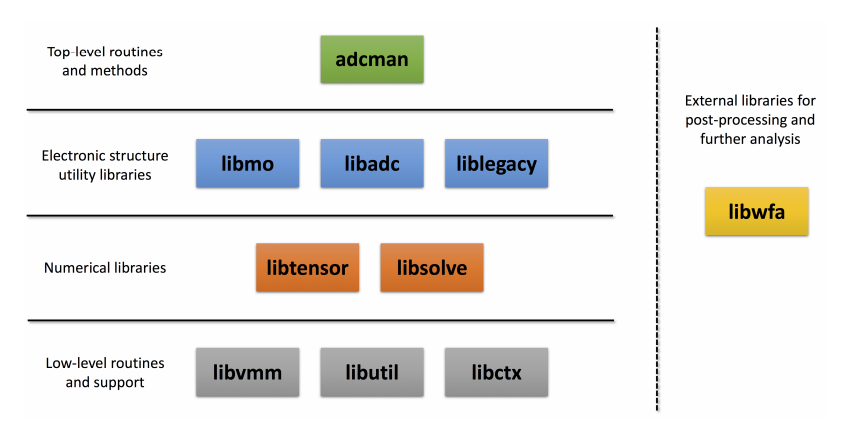
\includegraphics[width=\textwidth]{./figures/adcman.png}
	\caption{Overview of implementation of ADC methods in \emph{Q-Chem}}
	\label{codestucture}
\end{figure}

Then I will explain the overall code structure and then focus on my implementation part.
Finally I will present the results calculated by my implementation and compare them with CCSD.

\section{Code Overview and Structure}
The overview of implementation of ADC methods is in Fig. \ref{codestucture}.
All modules are written in the object-oriented C++ programming language. 
The adcman module contains all top-level routines and methods necessary for an ADC calculation. 
It coordinates the calculation process, sets up the solver and writes the results into an output file.
I implemented restricted calculation of EA part in adcman.

The next sub-level contains electronic structure related libraries and utilities.
\emph{liblegacy} is the gateway between the ADC code and the Q-Chem interface.
These routines help to import data from other Q-Chem modules, for example all SCF results and MOs, which are needed for the ADC calculation.
The \emph{libmo} module contains routines to set up the MO spaces, integrals and symmetry using the information imported from Q-Chem via the \emph{liblegacy} interface.
Hence, both \emph{libmo} and \emph{liblegacy} are important for ADC calculations, because all integrals and Fock-matrix elements are indexed and created corresponding to the additional restriction of the core space.
In the \emph{libadc} module, all ADC equations are implemented explicitly.
I also implemented restricted calculation of EA part in \emph{libadc}.

Furthermore, \emph{libmo} transforms the imported data in a format being compatible to the \emph{libtensor} \cite{libtensor} interface, which can be called the heart of the albegraic computation, since it contains all numerical routines to perform tensor algebra, which is the most time-consuming part all most of the quantum chemistry calculations.
\emph{libtensor} is specially designed for Post-Hartree-Fock electronic structure methods by including consideration of symmetries in the tensor structure.
These symmetries include Abelian point group symmetry, spin symmetry and other inner symmetry like that of two-electron integrals.
\begin{equation}
	\langle i j\| a b\rangle=-\langle j i\| a b\rangle=-\langle i j \| b a\rangle=\langle j i\| b a\rangle
\end{equation}
Thus, tensors of arbitrary order and size are stored in a blockwise manner to different kinds of symmetry to limit the amount of required memory and decrease the time needed.
The tensor operations in \emph{libtensor} are fully parallelized and efficiently implemented.

The second important numerical library is \emph{libsolve}, which contains all routines of
generic solvers, e.g the Davidson algorithm, which are called from the top-level adcman
routines. \emph{libsolve} is also based on the \emph{libtensor} interface. At last, there are low-level
routines, which are responsible for support and operations in the background. The libvmm
routines manage the virtual memory, while \emph{libctx} is a context manager based on key-value
mapping of data objects. All imported or generated objects, e.g. integrals, keywords,
tensors, vectors, etc., are stored in the context and can be easily accessed by other routines.
The libutil library contains further low-level machine-dependent routines.

The procedure of ADC calculation states as follows:
\begin{enumerate}
	\item A HF calculation is performed, and all information including one-electron integrals, two-electron integrals, MOs, eigenvalues, Overlap matrix, Fock matrix and point group symmetry are imported through \emph{libledacy} interface.
	\item All tensors calculated in the previous step are transformed from atomic orbital (AO) basis to MO basis by \emph{libmo} module.
	\item MP2 calculation is performed and results are printed.
	\item ADC secular matrix is constructed from the tensors in MO basis.
	\item Guess vectors which are required by Davidson algorithm are set up with correct symmetry.
	\item Davidson solver is started.
	\item When convergence requirements are met, ADC energies and transition amplitudes are printed.
	\item Other information required by adcman are printed.
\end{enumerate}

\section{Implementation of Non-dyson ADC}

\subsection{Implementation of ADC Secular Matrix}

We have illustrated the \emph{libtensor} library which can efficiently and conveniently realize tensor algebra.
From Eq \ref{KCeigen}, our final purpose is to calculate the eigenvalues and eigenvectors of ADC secular matrix.
However, usually we do not ask for all the eigenvalues and eigenvectors.
Instead, people are only interested in the few states with lowest energies.
Thus, full diagonalization will waste much effort on eigenstates that we are not interested in.
To solve this problem, we can use Davidson algorithm, which can determine eigenstates one by one with lower algorithmic complexity.
Since Davidson algorithm works by performing matrix vector product rather than direct access to matrix elements, we can rewrite the ADC secular matrix to matrix vector product form, i.e. calculate the result $W$ of matrix vector product when a vector $Y$ is given.

Before writing down the ADC secular matrix, we introduce some symbols:
\begin{equation}
	\begin{aligned}
		\langle pq \| rs \rangle&=V_{pq[rs]}
		\\
		\mathrm{t}_{\text { ijab }}&=\frac{\langle i j\| a b\rangle}{\varepsilon_{a}+\varepsilon_{\mathrm{b}}-\varepsilon_{i}-\varepsilon_{j}}
	\end{aligned}
\end{equation}

Up to second order, ADC secular matrix of ionization potential calculation is
\begin{equation}
	\mathrm{W}_{i}=\sum_{j} \mathrm{I}_{i j}^{(1)} \mathrm{Y}_{j}-\frac{1}{\sqrt{2}} \sum_{j k b}\langle j k\| b i\rangle Y_{j k b}
\end{equation}
for 1h part, where
\begin{equation}
\mathrm{I}_{i j}^{(1)}=-f_{i j}+\frac{1}{4}\left(1+\hat{\mathrm{P}}_{i j}\right) \sum_{a b k} t_{i k a b}\langle j k \| a b\rangle
\end{equation}
and
\begin{equation}
	\mathrm{W}_{i j a}=\sum_{\mathrm{b}} f_{a b} Y_{i j b}-\left(1-\hat{\mathrm{P}}_{i j}\right) \sum_{k} f_{i k} \mathrm{Y}_{k j a}+\frac{1}{\sqrt{2}} \sum_{k}\langle i j\| k a\rangle \mathrm{Y}_{k}
\end{equation}
for 1p-2h part.

Up to second order, ADC secular matrix of EA calculation is
\begin{equation}
	\mathrm{W}_{a}=\sum_{b} \mathrm{I}_{a b}^{(1)} \mathrm{Y}_{b}+\frac{1}{\sqrt{2}} \sum_{b c j}\langle b c\| j a\rangle Y_{b c j}
\end{equation}
for 1p part, where
\begin{equation}
\mathrm{I}_{a b}^{(1)}=-f_{a b}-\frac{1}{4}\left(1+\hat{\mathrm{P}}_{a b}\right) \sum_{i j c} t_{i j a c}\langle b c \| i j\rangle
\end{equation}
and
\begin{equation}
	\mathrm{W}_{a b i}=\sum_{\mathrm{b}} f_{i j} Y_{a b j}-\left(1-\hat{\mathrm{P}}_{a b}\right) \sum_{c} f_{a c} \mathrm{Y}_{c b i}-\frac{1}{\sqrt{2}} \sum_{c}\langle a b\| c i\rangle \mathrm{Y}_{c}
\end{equation}
for 1h-2p part.

The implementation of ADC secular matrix is by a class \emph{adc2\_matrix}:

\lstinputlisting[language=C++]{./code/adc2matrix.h}

\subsection{Implementation of Setting up Guess Vectors}

Before the Davidson algorithm starts, guess vectors need to be set up for the first matrix vector product.
Usually, the setting up of guess vectors should be subjected to some principles: computationally cheap and close to the final eigenvectors.
A simple idea is to use eigenvectors of some simple approximation of the ADC secular matrix.
In the implementation in Q-Chem, the approximation of second order ADC secular matrix is chosen to be the diagonal elements.
Since people usually care about the states with lowest enegies, the guess vectors should be chosen to be those with smallest diagonal elements.
Mathmatically, if $d_a=K_{aa}+C_{aa}$, and the $n$ smallest elements are $d_{k_1}<d_{k_2}< \dots <d_{k_n}$, then the $m$th guess vector should be 
\begin{equation}
	v^m_p=\delta_{p, k_m}
\end{equation}

Of course, we will get correct results if we set up guess vectors in the above way.
However, since Hamiltonian is commutable with total spin operator $S^2$, it is often required the diagonalization of Hamiltonian also diagonalizes $S^2$.
Thus, it is required that the initial guess vectors should have correct spin symmetry.
In addition, the 1h-2p guess vectors themselves has permutation symmetry
\begin{equation}
	V_{abi}=-V_{bai}
\end{equation}
, which is easy to deal with. Thus we will focus on spin symmetry of guess vectors.

For restricted calculation, electrons in ground state are always paired, thus the EA does not depend on whether alpha or beta electron is added, thus we can always choose it to be alpha electron.
Thus, the final state will be restricted to $m_s=\frac{1}{2}$.

For 1p guess vectors, there is no choice for spin since the added electron must be spin spin, and thus
\begin{equation}
	v^m_{a s}=\delta_{a, k_m} \delta_{s, \alpha}
\end{equation}
where $s$ is the spin of orbital a.

For 1h-2p guess vectors, there are two options:
\begin{itemize}
	\item One particle is alpha, one particle is beta, and the hole is beta.
	\item All two particles and the hole are alpha.
\end{itemize}

Thus there are totally three configurations (two for the first case and one for the second case).
To correcctly set up spin symmetry of guess vectors, we need to form linear combinations of these three configurations that are diagonal under $S^2$.
In fact, the coefficients of the linear combinations are refered as Clebsch-Gordan coefficients.
By refering to table of Clebsch-Gordan coefficients, the three final spin states reads:
\begin{equation}
	\begin{array}{|l|l|}
		\hline
		S=\frac{1}{2} & \sqrt{\frac{1}{2}} \ket{\alpha_p \beta_p \beta_h} - \sqrt{\frac{1}{2}} \ket{\beta_p \alpha_p \beta_h}
		\\
		\hline
		S=\frac{1}{2} & \sqrt{\frac{2}{3}} \ket{\alpha_p \alpha_p \alpha_h} - \sqrt{\frac{1}{6}} \ket{\alpha_p \beta_p \beta_h} - \sqrt{\frac{1}{6}} \ket{\beta_p \alpha_p \beta_h}
		\\
		\hline
		S=\frac{3}{2} & \sqrt{\frac{1}{3}} \ket{\alpha_p \alpha_p \alpha_h} + \sqrt{\frac{1}{3}} \ket{\alpha_p \beta_p \beta_h} + \sqrt{\frac{1}{3}} \ket{\beta_p \alpha_p \beta_h}
		\\
		\hline
	\end{array}
\end{equation}

The above tables works when the spacial orbital of two particles are different, otherwise they must have different spins, which means the second case is not allowed.
In such situation, the two paricles are paired, and will not contribute to the total spin.
Thus it reduces to the 1p case.

To summarize, if $a \neq b$, the first guess vector for spin $\frac{1}{2}$ is
\begin{equation}
	\begin{array}{ll}
		V_{a \alpha, b \beta, i \beta}=\frac{1}{2} & V_{b \beta, a \alpha, i \beta}=-\frac{1}{2} 
		\\
		V_{a \beta, b \alpha, i \beta}=-\frac{1}{2} & V_{b \alpha, a \beta, i \beta}=\frac{1}{2} 
	\end{array}
\end{equation}
the second guess vector for spin $\frac{1}{2}$ is 
\begin{equation}
	\begin{array}{ll}
		V_{a \alpha, b \alpha, i \alpha}=\sqrt{\frac{1}{3}} & V_{b \alpha, a \alpha, i \beta}=-\sqrt{\frac{1}{3}} 
		\\
		V_{a \alpha, b \beta, i \beta}=-\sqrt{\frac{1}{12}} & V_{b \beta, a \alpha, i \beta}=\sqrt{\frac{1}{12}} 
		\\
		V_{a \beta, b \alpha, i \beta}=-\sqrt{\frac{1}{12}} & V_{b \alpha, a \beta, i \beta}=\sqrt{\frac{1}{12}} 
	\end{array}
\end{equation}
the guess vector for spin $\frac{3}{2}$ is
\begin{equation}
	\begin{array}{ll}
		V_{a \alpha, b \alpha, i \alpha}=\sqrt{\frac{1}{6}} & V_{b \alpha, a \alpha, i \beta}=-\sqrt{\frac{1}{6}} 
		\\
		V_{a \alpha, b \beta, i \beta}=\sqrt{\frac{1}{6}} & V_{b \beta, a \alpha, i \beta}=-\sqrt{\frac{1}{6}} 
		\\
		V_{a \beta, b \alpha, i \beta}=\sqrt{\frac{1}{6}} & V_{b \alpha, a \beta, i \beta}=-\sqrt{\frac{1}{6}} 
	\end{array}
\end{equation}
if $a=b$, the first guess vector for spin $\frac{1}{2}$ is
\begin{equation}
	\begin{array}{ll}
		V_{a \alpha, b \beta, i \beta}=\frac{1}{2} & V_{b \beta, a \alpha, i \beta}=-\frac{1}{2} 
		\\
		V_{a \beta, b \alpha, i \beta}=-\frac{1}{2} & V_{b \alpha, a \beta, i \beta}=\frac{1}{2} 
	\end{array}
\end{equation}
the second guess vector for spin $\frac{1}{2}$ is 
\begin{equation}
	\begin{array}{ll}
		V_{a \alpha, b \beta, i \beta}=\frac{1}{2} & V_{b \beta, a \alpha, i \beta}=\frac{1}{2} 
		\\
		V_{a \beta, b \alpha, i \beta}=\frac{1}{2} & V_{b \alpha, a \beta, i \beta}=\frac{1}{2} 
	\end{array}
\end{equation}

For unrestricted case, it is much more complicated.
Although I do not implement it, it does not hurt to discuss a little about this.

Consider the ground state of a system with $p$ net positive charge, in which $p_{\alpha}$ are spin alpha while $p_{\beta}$ are spin beta.
After affinity of an electron, which could be either spin alpha or spin beta.
Thus, the general question is the linear combination of $n_{\alpha}$ alpha spins and $n_{\beta}$ beta spins, where
\begin{equation}
	\begin{array}{lll}
		n_{\alpha}=p_{\alpha} + 1, & n_{\beta}=p_{\beta} & \text{if added alpha electron}
		\\
		n_{\alpha}=p_{\alpha}, & n_{\beta}=p_{\beta} + 1 & \text{if added beta electron}
	\end{array}
\end{equation}

The $n=n_{\alpha} + n_{\beta}$ electrons will genrate $2^n$ configurations.
However, Clebsch-Gordan coefficients only works for addition of two spins.
Thus, an recursive approach is needed to deal with the $n$ spin case.

\section{Results of Calculation}

In this section, I will present a benchmark calculation of the EA-ADC(2) method.
The calculated results are compared with HF, DFT with B3LYP functional and CCSD.
CCSD is used for comparison because CCSD is a widely used Post-Hartree-Fock method to include consideration of electron correlation, which is very reliable.
HF and DFT are used for comparison to show that ADC can perform better than these low-level results, otherwise we don't need these high-level methods, which are computationally more expensive.
For this benchmark calculation, small moleculars 
$\text{H}_2\text{O}$, $\text{NH}_3$, $\text{CO}_2$, $\text{LiH}$,
$\text{LiF}$, $\text{N}_2\text{O}$, $\text{CH}_4$,
$\text{C}_2\text{H}_6$, $\text{CH}_2\text{O}$, $\text{HCN}$ are chosen, and the basis set is chosen to be 6-31g.
The results of HF and DFT are obtained by subjecting the ground state energy of original molecule and anion with -1 charge.
Since both HF and DFT are size consistent, it will not cause problem of size consistency.

\begin{table}
	\centering
	\caption{first EA of small molecules under cc-pVTZ basis}
	\label{firstEA}
\begin{tabular}{|c|c|c|c|c|}
	\hline
	Molecules              & HF    & B3LYP & ADC(2) & CCSD  \\ \hline
	$\text{CO}_2$          & -4.64 & -3.46 & -3.47  & -3.73 \\ \hline
	LiF                    & 0.14  & 0.29  & 0.18   & 0.17  \\ \hline
	LiH                    & 0.08  & 0.25  & 0.12   & 0.13  \\ \hline
	$\text{N}_2\text{O}$   & -2.95 & -2.8  & -2.8   & -3.22 \\ \hline
	$\text{H}_2\text{O}$   & -3.72 & -2.93 & -3.27  & -3.31 \\ \hline
	$\text{NH}_3$          & -3.62 & -2.78 & -3.08  & -3.13 \\ \hline
	$\text{CH}_4$          & -3.82 & -2.96 & -3.27  & -3.31 \\ \hline
	$\text{C}_2\text{H}_2$ & -4.17 & -2.93 & -3.33  & -3.5  \\ \hline
	HCN                    & -3.71 & -2.99 & -3.09  & -3.29 \\ \hline
	$\text{CH}_2\text{O}$  & -2.15 & -1.47 & -1.62  & -1.92 \\ \hline
\end{tabular}
\end{table}
\begin{figure}[ht]
	\centering
	\begin{subfigure}[b]{0.42\linewidth}
		\centering
		\includegraphics[width=\linewidth]{./figures/higher/C2H2.pdf}
	\end{subfigure}
	\begin{subfigure}[b]{0.42\linewidth}
		\centering
		\includegraphics[width=\linewidth]{./figures/higher/CH2O.pdf}
	\end{subfigure}
	\begin{subfigure}[b]{0.42\linewidth}
		\centering
		\includegraphics[width=\linewidth]{./figures/higher/CH4.pdf}
	\end{subfigure}
	\begin{subfigure}[b]{0.42\linewidth}
		\centering
		\includegraphics[width=\linewidth]{./figures/higher/CO2.pdf}
	\end{subfigure}
	\begin{subfigure}[b]{0.42\linewidth}
		\centering
		\includegraphics[width=\linewidth]{./figures/higher/H2O.pdf}
	\end{subfigure}
	\begin{subfigure}[b]{0.42\linewidth}
		\centering
		\includegraphics[width=\linewidth]{./figures/higher/HCN.pdf}
	\end{subfigure}
	\begin{subfigure}[b]{0.42\linewidth}
		\centering
		\includegraphics[width=\linewidth]{./figures/higher/LiF.pdf}
	\end{subfigure}
	\begin{subfigure}[b]{0.42\linewidth}
		\centering
		\includegraphics[width=\linewidth]{./figures/higher/LiH.pdf}
	\end{subfigure}
	\begin{subfigure}[b]{0.42\linewidth}
		\centering
		\includegraphics[width=\linewidth]{./figures/higher/N2O.pdf}
	\end{subfigure}
	\begin{subfigure}[b]{0.42\linewidth}
		\centering
		\includegraphics[width=\linewidth]{./figures/higher/NH3.pdf}
	\end{subfigure}
	\caption{First 10 EAs calculated by ADC(2) and CCSD on small molecules}
	\label{higher}
\end{figure}
On the other hand, choice of appropriate basis is very important for EA calculation.
The reason is that anions bind their outermost electrons rather weakly, and hence their valence-range electron densities are diffuse, which means that the use of diffuse functions is an important requirement for basis in EA calculation, and also means that a large basis space is needed to achieve accurate results. One of the basis that satisfying this requirement is cc-pVXZ basis (X=D/T/Q/5 \dots). \cite{newpaper}

We first calculate the first EA energy for these molecules.
In this calculation, cc-pVTZ basis and CCSD are used for an accurate geometry optimization and then cc-PVTZ basis is used for EA calculation.
The results are shown in Table \ref{firstEA}

We can see from the results that ADC(2) matches well with CCSD (mean derivation is 0.15 eV), while both HF and DFT give great derivation (mean derivations are 0.34 eV for HF and 0.39 eV for DFT).
We can also find that HF tends to underestimate EA, and DFT tends to overestimate EA.

Then we compare higher order electron affinities calculated by ADC(2) and CCSD on these small molecules.
Results are shown in Fig. \ref{higher}
As is shown in the figure, ADC(2) results match well with CCSD for the first few EAs among all the molecules.
However, they give large errors for higher orders of EAs, and ADC almost always gives lower EAs for these states.
We can also find that generally, disagreements comes later for large molecules (CO$_2$, N$_2$O and C$_2$H$_2$).

If we look into the amplitudes of 1p and 1h-2p parts, we can find that when a state is dominated by 1p part, ADC(2) and CCSD usually give similar results; however,when it is dominated by 1h-2p part, two theories disagree with a large probability.
This means that the ADC(2) give good results for 1p part but bad result for 1h-2p part, and it usually overestimate the energies for 1h-2p part.
Then we will analyze the reason for this.
Eq \ref{generalTEO} in ISR theory tells us that in the case of ADC(2), TEO of 1p part is second order, while TEO of 1h-2p part is zeroth order.
Thus, ADC(2) gives larger error for 1h-2p results while describes 1p part accurately, compared with CCSD.

On the other hand, we can see from the structure of ADC(2) secular matrix \ref{ADC2} that only $K_2$ is included for 1h2p-1h2p part, thus there is no mix between 1h2p states, which can not effectively decrease energies.
This problem will be solved in ADC(3), since $C^1_{11}$ is also included in 1h2p-1h2p part, and thus TEO for 1h2p states is second order, which is much better.

Another problem for these results is that first EAs of all molecules except Li$_H$ and Li$_F$ are negative, which means that such states are not stable and the anions will automatically decompose into a neutral and a free electron, which is totally unphysical.

This problem comes from two parts.
The first part is finite basis, and the second part is incorrect result of electron correlation.
The first part can principly be solved by complete basis set (CBS).
One famous CBS is cc-pVXZ basis \cite{CBS}, which should give asymptotic results when $X \rightarrow \infty$.
Then we perform calculations for LiH, LiF, CO$_2$ and N$_2$O under these basis.
The results are shown in Table \ref{ccpVXZ}.
\begin{table}
	\centering
	\caption{first EA calculated by ADC(2) and CCSD for cc-pVDZ, cc-pVTZ cc-pVDZ}
	\label{ccpVXZ}
	\begin{tabular}{|c|c|c|c|c|c|c|}
		\hline
		\multirow{2}{*}{Molecules} & \multicolumn{3}{c|}{ADC(2)} & \multicolumn{3}{c|}{CCSD}   \\ \cline{2-7} 
								   & cc-pVDZ & cc-pVTZ & cc-pVQZ & cc-pVDZ & cc-pVTZ & cc-pVQZ \\ \hline
		LiH                        & 0.06    & 0.12    & 0.20    & 0.07    & 0.13    & 0.20    \\ \hline
		LiF                        & 0.12    & 0.18    & 0.26    & 0.11    & 0.17    & 0.25    \\ \hline
		CO$_2$                     & -4.97   & -3.47   & -2.52   & -5.21   & -3.73   & -2.73   \\ \hline
		N$_2$O                     & -3.55   & -2.80   & -2.48   & -3.92   & -3.22   & -2.92   \\ \hline
	\end{tabular}
\end{table}
As we can see in the results, the first EA increases when $X$ increases among all of the molecules, which means basis set plays a very imporant role to get positive EAs.
However, cc-pVXZ is a really large basis set, thus a cc-pV5Z is difficult for these molecules and is not given in this benchmark calculation.

For the second part of the reason, which is incorrect electron correlation, it still remains unsolved until now and is one of the center problems of electronic structure.
Many methods are also under development to solve this problem.
Thus, it is not surprising to see that both ADC(2) and CCSD sometimes give bad results.


\chapter{Conclusion}
In this thesis, I first introduced history of development of electronic structure and important methods under Born-Oppenheimer and non-relativistic approximation.
Hartree-Fock, as the lowest-level method among all of them, usually functions at the starting point, and both Post-Hartree-Fock methods and DFT are based on Hartree-Fock.
Hartree-Fock also functions as a formal definition of MO, and all other corrections are refered to as electron correlation.
Among Post-Hartree-Fock methods, CI is conceptually the simplest but is neither efficient nor give size consistency, which is a very important property for electronic structure methods to give self-consistent results for many important chemical processes.
CC solve the problem of size consistency by introducing an exponential excitation operator, which also includes electron correlation by a more efficient way.
However, the nonlinear equations that CC has to solve makes it computationally expensive.
MP perturbation theory is also a kind of Post-Hartree-Fock methods, which views total Hamiltonian excluding Hartree-Fock Hamiltonian as perturbation and then expands it in series.
In addition to Post-Hartree-Fock methods, DFT is also introduced, which uses an unknown functional to represent all electron correlation effects based on Hohenberg-Kohn theorem.

Then I introduced the theory of ADC, starting from important mathematical and physical backgrounds.
Second quantization, which is the language used by many-body field theory, use creation and annihilation operators as basic elements and thus include particle identity automatically.
Green function, which originally appears in classical field theory, is extended to quantum field theory.
By creation and annihilation operators, the definition of Green function is given in the time ordering operator form and is then proves that all its poles are exactly ionization potentials and electron affinities by spectral representation, and can also relate to ground state energy.
Free Green function was calculated as the zeroth order of Green function.
Afterwards, by the introduction of interaction picture, Gell-Mann and Low theorem can be applied to expand Green function into perturbation series, which are represented by time ordered products.
Then Wick's theorem is introduced, which presents an approach to calculate time ordered products.
By taking advantage of the regularity of time ordered products calculation, Feynman diagram can be introduced to visualize all perturbation terms and can also restore analytical expressions from diagrams.
From linked-cluster theorem, we know that only linked diagrams need to be included.
Feynman rules are given for systematically construct any particular order of Green function.

With the background of second quantization, Green function and Feynman diagram, ADC is then presented.
The concept of self-energy is first defined, which gives an approach to perform a partial summation over infinite orders.
Thus the problem of finding poles of Green functions is transformed to an eigenvalue problem of Dyson-ADC secular matrix, which can also be expanded into series.
However, ionized part and anionized part are coupled in Dyson-ADC, making it difficult to solve.
Thus, a Non-dyson approach is presented to solve this problem by directly expanding Green function to series after some mathematical transformation, which preserves the summation to infinite orders.

To better understand the efficiency and size consistency of Non-dyson ADC, ISR is introduced as a special way to construct many-body basis.
It is proved that Hamiltonian under ISR is exactly Non-dyson ADC secular matrix.
From ISR approach, it can be proved that Non-dyson ADC follows canonical order relation, which guarantees its computational efficiency, and also separability, which then leads to its size consistency property.

Then I described my implementation of Non-dyson EA-ADC(2) in \emph{adcman}.
The code structure of \emph{adcman} is given and then the procedure is presented.
For implementation, ADC secular matrix is given.
It is illustrated that 1h-2p guess vectors must be set correctly to be subjected to correct spin symmetry.

Finally, results of ADC benchmark calculation are performed and compared with HF, DFT (B3LYP) and CCSD.
It is shown that for 1p states, ADC(2) matches well with CCSD, while HF and DFT give a very large error.
However, for 1h-2p states, ADC(2) shows a large derivation with CCSD, which is caused by low-level description of 1h2p-1h2p in ADC(2) secular matrix, which can be solved in ADC(3).

%\input{chapters/floats}
%\input{chapters/math}
%\input{chapters/citations}
\bibliography{bib/ustc.bib}
%\appendix
%\input{chapters/complementary}

\backmatter
%\input{chapters/publications}

\end{document}
